% M. S. Tsoeu (2011), University of Cape Town <mohohlo.tsoeu@uct.ac.za>

% This is a project report templace document created for EEE4022FS students at the University of Cape Town.
%
% This file should be is processed with ``pdflatex`` and might need a few modifications if a different processor is chosen.

% Modified by Othniel Konan (2017), University of Cape Town <knnoth001@myuct.ac.za>


\documentclass[a4paper,12pt]{report}

%Include packages you need to use here

\usepackage[top = 1in, bottom = 1in, left = 1.5in, right = 1in]{geometry}
\usepackage{graphicx}
\usepackage{fancyhdr}
\usepackage{amsmath, amsthm, amssymb}
\usepackage{lastpage}
\usepackage{subcaption}	% multiple figures 
\usepackage{lscape}
\usepackage{hyphenat}
\usepackage{setspace}
\usepackage{hyperref}
\usepackage{color}
\usepackage[dvipsnames]{xcolor}
\usepackage{pdflscape}	% landscape
\usepackage{cleveref}	% multiple references
\usepackage{multirow}	% merge rows
%\usepackage{titlesec}
\usepackage{dirtytalk}
\graphicspath{{./figures/}}

% Include page formatting here. 
\parskip = 6pt
\parindent = 0mm
\renewcommand{\headrulewidth}{0pt}
\rhead[]{\thesection}
\lhead[\thechapter]{}

\begin{document}

% This section formats the title page of the Report.
\thispagestyle{empty}
{\Huge \begin{center}
% Modify the line below to insert your title.
\textcolor{MidnightBlue}{\textbf{NeoPixel Sunrise Clock}}
\vskip 1mm
\color{MidnightBlue} \hrule
% Modify the line below to insert your subtitle.
{\Large An intelligent bedside clock}
\end{center}}

\vskip 5mm
\begin{center}

\includegraphics[scale = 0.3]{uctLogo.png}
\end{center}

\vskip 5mm
\begin{center}
Presented by:\\
\textbf{Othniel Konan}\\		% Insert your name here
KNNOTH001\\
Dept. of Electrical and Electronics Engineering\\University of Cape Town

\end{center}

\vskip 10mm
\begin{center}
Prepared for:\\
\textbf{Dr. Simon Winberg \& Mr. Justin Pead}\\ 		% Insert your supervisor's name here.
Dept. of Electrical and Electronics Engineering\\University of Cape Town
\end{center}


\vskip 10mm
\begin{center}
Submitted to the Department of Electrical Engineering at the University of Cape Town in partial
fulfilment of the academic requirements for a Bachelor of Science degree in Electrical and Computer Engineering

\end{center}


\vskip 5mm
\begin{center}{\bf \today}
\end{center}

\vskip 5mm
\begin{center}
\textbf{Key Words:} Neopixels, Circadian rhythm, STM32, Blue light, Nextion, MIT App Inventor
\end{center}


\newpage
\thispagestyle{empty}
\mbox{}
\newpage

\onehalfspacing
\nohyphens{
\thispagestyle{empty}
\vskip 40mm


% Please leave the declaration as it is (Standard UCT declaration).
{\Large Declaration}\\
\hrule

\vskip 10mm
\begin{enumerate}
\item I know that plagiarism is wrong. Plagiarism is to use another's work and pretend that it is one's
own.
\item I have used the IEEE convention for citation and referencing. Each contribution to, and quotation in,
this report from the work(s) of other people has been attributed, and has been cited and
referenced.
\item This report is my own work.
\item I have not allowed, and will not allow, anyone to copy my work with the intention of passing it off
as their own work or part thereof.
\end{enumerate}
\vskip 10mm
Signature: \ldots\ldots\ldots\ldots\ldots\ldots\ldots\ldots\ldots 
\\Othniel Konan		% Chante this line to your name.
\vskip 6mm
Date: \ldots\ldots\ldots\ldots\ldots\ldots\ldots\ldots\ldots\ldots .


\fancyfoot[C]{\thepage}
\pagestyle{plain}
\newpage
\pagenumbering{roman}

{\Large Acknowledgments}\\
\hrule

\newpage

{\Large Abstract}\\
\hrule

% Place your abstract here.
\begin{itemize}
\item Open the {\bf Project Report Template.tex} file and carefully follow the comments (starting with \%).
\item Process the file with {\bf pdflatex}, using other processors may need you to change some features such as graphics types.
\item Note the files included in the  {\bf Project Report Template.tex} (with the .tex extension excluded). You can open these files separately and modify their contents 
or create new ones.
\item Contact the latex namual for more features in your document such as equations, subfigures, footnotes, subscripts \& superscripts, special characters etc.
\item I recommend using the {\bf kile} latex IDE, as it is simple to use.
\end{itemize}

\newpage
\tableofcontents

\newpage
\listoffigures

\newpage
\listoftables

% Page formatting, to place section titles as headers of odd pages and Chapter titles as headers of even pages.
\newpage
\fancyhead[RE,LO]{}
\fancyhead[LE]{\leftmark}
\fancyhead[RO]{\rightmark}
\pagestyle{fancy}

\pagenumbering{arabic}

% THe files included below are .tex files containing the respective chapters these are already created in this package and you can add to or modify them.
\chapter{Introduction}

\section{Background to the study}
A very brief background to your area of research. Start off with a general introduction to the area and
then narrow it down to your focus area. Used to set the scene \cite{smt2011}.
\section{Objectives of this study}
\subsection{Problems to be investigated}
Description of the main questions to be investigated in this study.
\subsection{Purpose of the study}
Give the significance of investigating these problems. It must be obvious why you are doing this study
and why it is relevant.

\section{Scope and Limitations}
Scope indicates to the reader what has and has not been included in the study. Limitations tell the
reader what factors influenced the study such as sample size, time etc. It is not a section for excuses as
to why your project may or may not have worked.

\section{Plan of development}
Here you tell the reader how your report has been organised and what is included in each
chapter.

{\bf I recommend that you write this section last. You can then tailor it to your report.}

\chapter{Literature Review}

This chapter reviews the research papers, articles, books and other relevant forms of research used in the design of the NPSC. It has been divided into the sections illustrated by \cref{fig:lit_rev}:
\begin{figure}[h!]
\centering
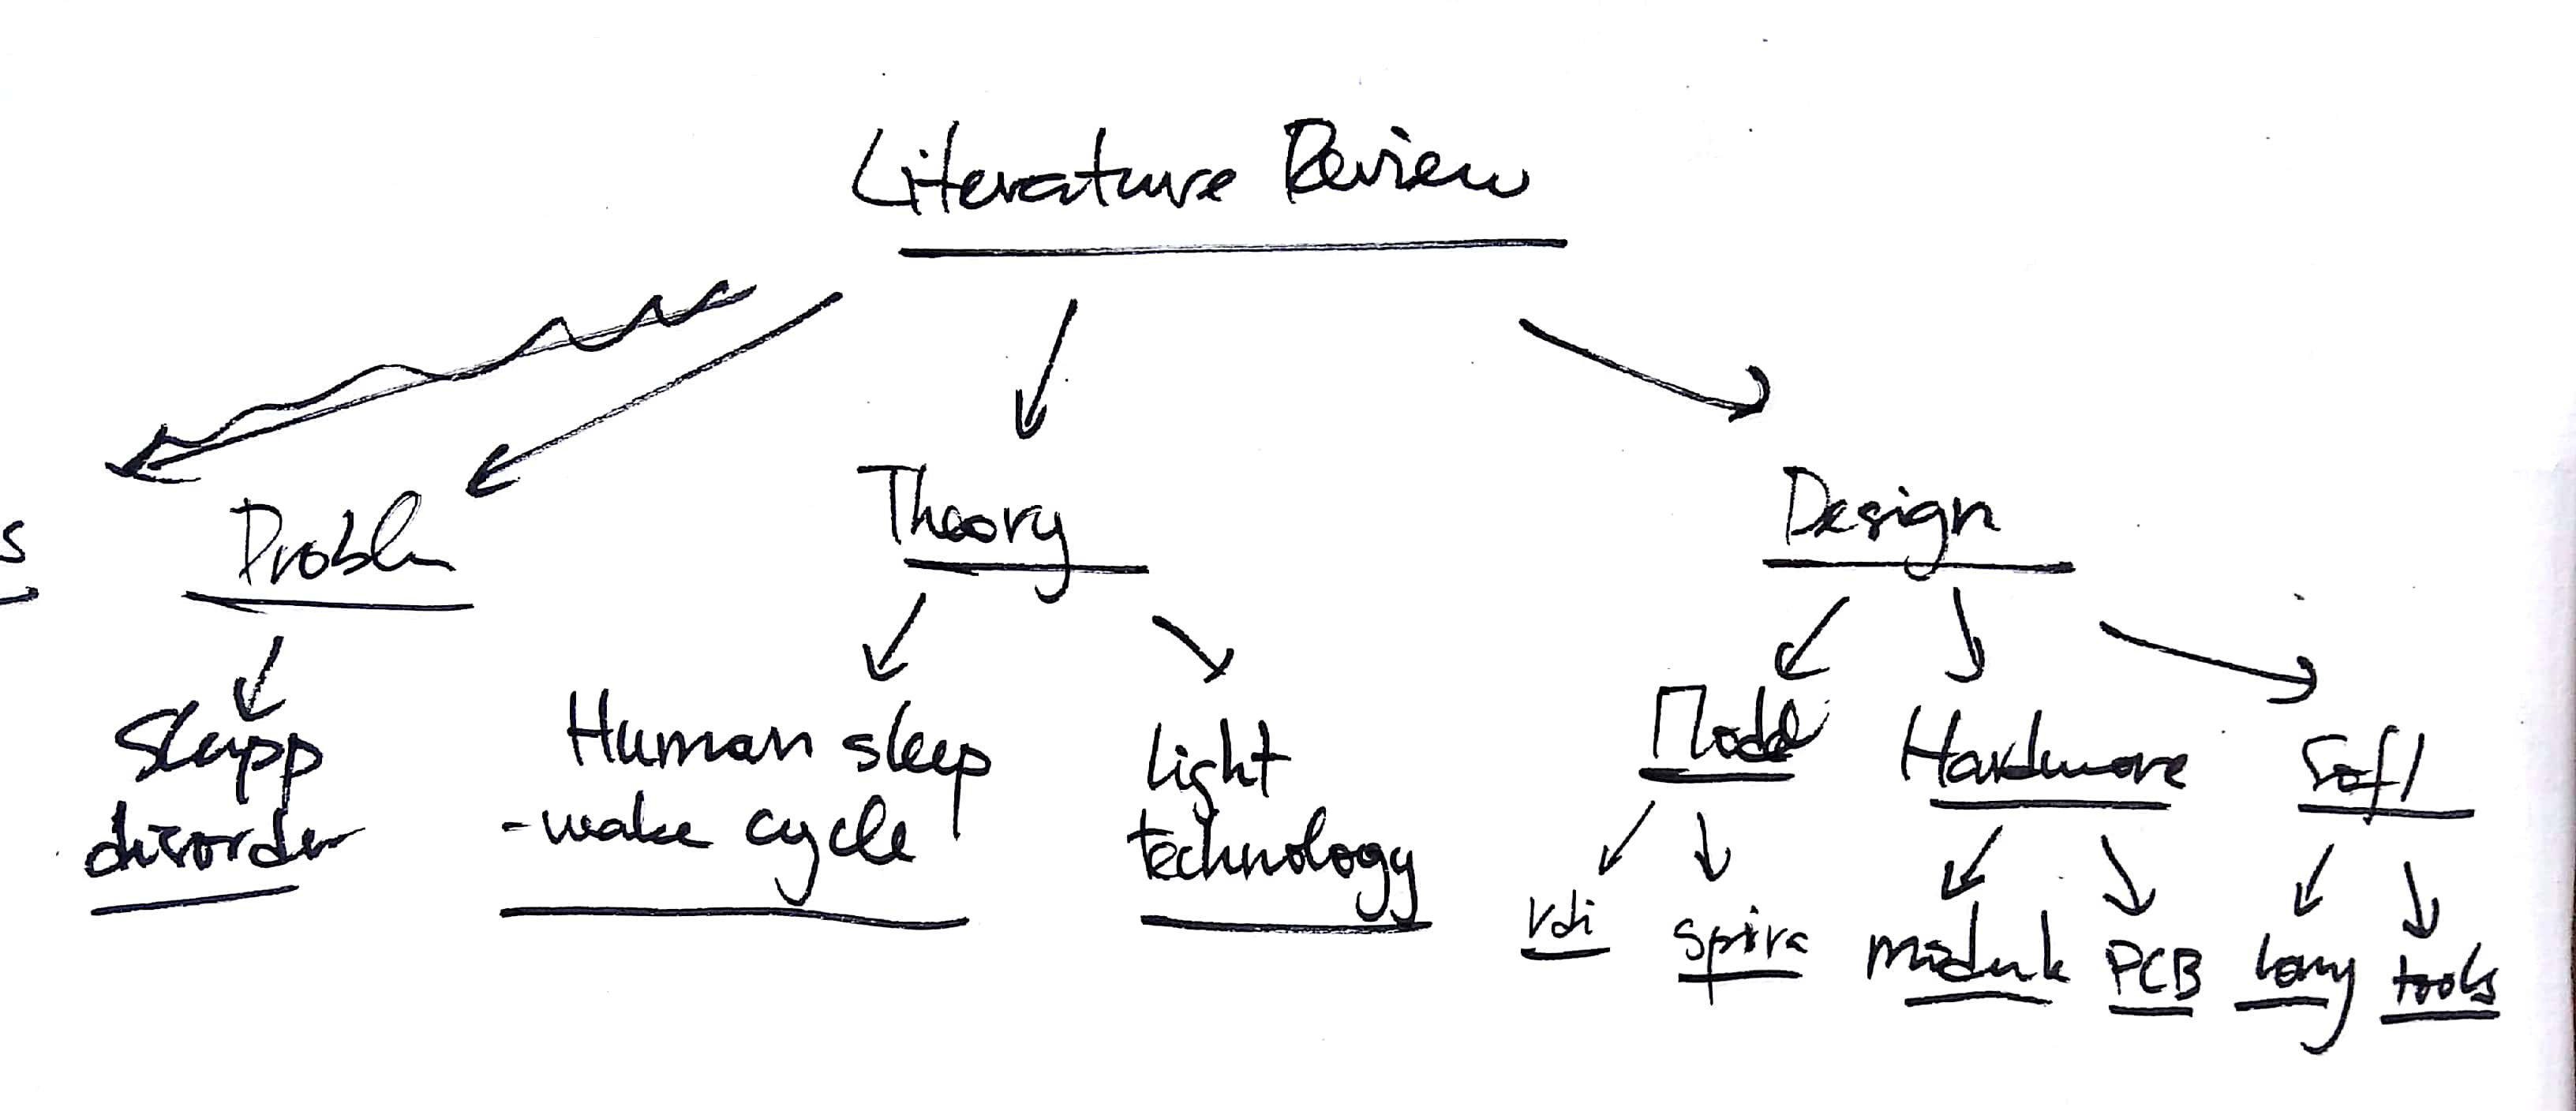
\includegraphics[scale=0.1]{lit_rev.jpg}
\caption{Overview and classification of the sections of the literature review.}
\label{fig:lit_rev}
\end{figure}
The literature review starts with an explanation of the problems to be solved, it continues by uncovering the theory behind these problems and ends with a review of the design methods, hardware components and software tools used in this project.

%%%%%%%%%%%%%%%%%%%%%%%%%%%%%%%%%%%%%%%%%%%%%%%%%%%%%%%%%%%%%%%%%%%%%%%%%%%%%%%%%%%%
% SECTION: The human sleep-wake cycle
%%%%%%%%%%%%%%%%%%%%%%%%%%%%%%%%%%%%%%%%%%%%%%%%%%%%%%%%%%%%%%%%%%%%%%%%%%%%%%%%%%%%
\section{The human sleep-wake cycle}

Human has many \say{internal clocks} among them is the master clock located in the suprachiasmatic nuclei. These internal clocks or endegenous clocks are internal mechanisms in organisms reponsible for the regulations of certain functions or activities. The master clock cheif among them, regulates the secretion of melatonin is affected by light. The creation of artifical light expecially LEDs have caused a disruption in the sleep-wake cycle. This section give an overview of the human internal clocks and how they are affected by light.

\subsection{The circadian rhythm}
Human seasonal behaviours are synchronised to the environment by \textbf{biological clocks} responsible for the creation of biological rhythms. Biological clocks which are composed of proteins that act reciprocally on the body's cells are the natural timing devices found in many organs. The discovery of the genes from these biological clocks responsible for the control of these rhythms was made by three scientists Jeffrey  C.  Hall,  Michael  Rosbash and Michael W. Young winners of the Nobel Prize in Physiology or Medicine \cite{sc2017}. Their discovery made in the 1980s led to advanced research on the role of the circadian rhythms.\\
Circadian rhythms are biological rhythms which follow the same pattern in absence of external cues (endogenous), are influenced by the presence of external stimuli (entertainable), oscillating roughly every 24h\footnote{it oxalates generally a period near 24h} over a range of physiological temperatures. In the presence of external stimuli -also known as \textit{zeitgebers}-, circadian rhythms synchronise their periodicity with these external stimuli. The zeitgebers of the circadian are the daily variation of the temperature and the dark/light cycle of the day.\\
Circadian rhythms have endogenous and exogenous components. Human placed in isolation without knowledge of the time continued exhibiting a circadian rhythm with their pacemakers notably the melatonin secretion, sleep-wake cycle, body temperature \cite{in1996}. These results prove the existence of endogenous components of the circadian rhythms as it illustrates the effects of these internal signal on the circadian rhythms. A similar study shows that when people are exposed to light at night time, a shift in their pacemakers \cite{ea2004} which is an evidence of the exogenous component of circadian rhythms. These exogenous components of the circadian rhythms have the ability affect positively and negatively our natural endogenous cycle. With light being what we are mostly daily exposed to, what is the influence of light on the circadian rhythms? 

\subsection{Internal circadian rhythms influenced by light}
Melatonin is the hormone produced by the pineal gland in the suprachiasmatic nuclei (SCN) which has a soporific effect and the ability to entertain the sleep-wake cycle. While melatonin itself is not the cause of a person sleeping, it however creates changes in a person's body that affect their sleepiness. \\
The pineal gland responsible for the secretion of the melatonin hormone is under the influence of one of the biological clocks, the master clock located in the SCN. The SCN receives visual information from the retinal-hypothalamic tract which entrains the SCN according to the photoperiod \cite{lig1994}. The SCN in turn activate a gene in the pineal cell (CREM) which produces a protein (ICER) needed for the production of melatonin. As a result, the secretion of pineal hormone melatonin tracks the light/dark cycle with its  secretion being high during the day and low during the night.  

\subsection{Quantitative and qualitative characteristics of light on melatonin production}
Many types of research have been done to understand the impact of light on the circadian rhythms especially the sleep-wake cycle. \\
Kathleen \textit{et al.} in their paper \textit{Blue light from light-emitting diodes elicits a dose-dependent suppression of melatonin in humans}\cite{bl2010}, provide details information on their finding of the effect of light on humans subject. Subjects used for the experiments were 5 males and 3 females with a mean of $23.9\pm0.5$ years, with each subject demonstrating normal colour vision. The lighting requirement was blue light of $\lambda_{max} = 469nm \pm 1nm $ with $\frac{1}{2}$ peak bandwidth$ = 26nm$ and a typical viewing distance of $35cm$. The subjects were blindfolded from midnight to 2 AM. From thereon, they were exposed to 90 min of blue light exposure followed by another dark exposure. Blood samples from the subject were taken from 2 AM at 30 min interval.From their experiment, they concluded that:
\begin{itemize}
\item \textit{Blue LED light has an increased melatonin suppression following an increase in exposure irradiance}
\item \textit{Blue LED light may have stronger suppressing effect than 4000K white fluorescent light.}
\end{itemize}
A similar study was previously made by George C. Brainard \textit{et al.} \cite{ac2001} used 72 healthy human subjects, with normal colour vision. The subjects composed of 37 females, 35 males, aged between 18 and 30 years (mean age of $24.5 \pm 0.3$ years), came from different ethnic (African, African Americans, Caucasians, Asian, Hispanic). The melatonin suppression action spectrum was formed using eight different wavelengths between $440nm$ and $600nm$ \textit{(440, 460, 480, 505, 530, 555, 575, 600)}. Using the same procedure as mentioned in the previous experiment, blood samples were taken at 30 min interval after 2 AM. The results of their research published in their paper \textit{Action Spectrum for Melatonin Regulation in Humans: Evidence for a Novel Circadian Photoreceptor} the following conclusion:
\begin{itemize}
\item \textit{Light irradiance greater or equal to $3.1 \mu W/cm^{2}$ evoke a significant melatonin supression}
\item \textit{Smaller wavelength monochromatic light have a greater change in \textit{Plasma Melatonin as Percent Change Control-Adjusted} for a fixed value of \textit{Photon density}} (\cite{ac2001} pp. 4-5).
\end{itemize}   

\subsection{Impact of light on human behaviour and sleep-wake cycle}
Among the Zeitgebers (natural phenomenon acting as a signal in the regulation of the circadian rhythm)  of the circadian rhythms, light is the major Zeitgebers and has important effects on the human sleep-wake cycle. A study on the \say{Circadian and Light Effects on Human Sleepiness-Alertness} made by Christian \textit{et al.}\cite{cir2014} shows that with nor phase lag or lead between the circadian rhythm and the sleep-wake cycle, subjective sleepiness and core body temperature have opposite behaviour (\cite{cir2014}, pp. 12, fig. 2.1). The human normal sleep-wake cycle is comprised of 8h of sleep and 16h of wakefulness \cite{is1995}. This cycle is naturally affected by the human activities but is highly influenced by light exposure. The study shows that office workers with bright blue office light have a better sleep-wake cycle than those with dim and warm office light. Furthermore, it shows that light exposure of sufficient intensity at night can reduce the secretion of melatonin with alerting response starting within the first 20mm. With the recent advance in LED technologies, humans are no longer following the natural light/dark cycle causing numerous sleep disorders. 

%%%%%%%%%%%%%%%%%%%%%%%%%%%%%%%%%%%%%%%%%%%%%%%%%%%%%%%%%%%%%%%%%%%%%%%%%%%%%%%%%%%%
% SECTION: LEDs technologies
%%%%%%%%%%%%%%%%%%%%%%%%%%%%%%%%%%%%%%%%%%%%%%%%%%%%%%%%%%%%%%%%%%%%%%%%%%%%%%%%%%%%
\section{Lighting technologies}

Light is capable of affecting the human sleep-wake cycle. However this impact can be used to reverse the negative impact of light on the sleep-wake cycle. This section introduces the different light technologies available and their use in regualting the human sleep-wake cycle. 

\subsection{Light}
The sun's electromagnetic radiation has a broad light spectrum ranging from  $100nm$ to $1mm$. After being filtered through the earth atmosphere, only certain portions of the spectrum are kept with the visible light spectrum having the maximum irradiance. Because the human circadian rhythms are automatically synchronised to the natural light-dark cycle, the characteristics of the sunlight are used as a benchmark in the emission of artificial light. These artificial lights are able to produce more or less the same wavelength as the sunlight but with much less irradiance.

\subsection{Type of light technologies}
Various light technologies have been developed over the years, their use and their usefulness in this project are detailed below. 
\subsubsection{Incandescent light}
These are the most common and least efficient light technology. It produces light by passing a high current through a wire filament producing warm light as it glows. These type of lights produce only a specific spectrum of light (warm light) besides they are not designed to be programmable. 
\subsubsection{Fluorescent light}
Light is produced by passing electricity through mercury vapour, the invisible light produced as a result of that interaction, connect with the coating of the glass emitting light. It produces all type of white light (warm, cool, daylight) with a good colour rendering. Compared to the incandescent light, it only produces one type of colour and it is not designed to be programmable.
\subsubsection{Halogen light}
It shares similarities with the incandescent light except that halogen gas is added to the glass. It produces a crisp white colour. As the previous technologies, it also produces one type of colour and it not designed to be programmed.
\subsubsection{Xeon light}
This type is another version of incandescent light with Xeon gas added to the glass instead, it produces a less yellow light. As the previous technologies, it also produces one type of colour and it not designed to be programmed.
\subsubsection{LED light}
This technology uses the passage of current through a diode to produce light. These light are very efficient and provide all sort of colour as well as cool and warm light. Moreover, their ability to work based on the passage on current allows these lights to be programmable. New LED technologies have a microcontroller which can be programmed the LEDs. 
\subsection{Light treatment of sleep disorder}
With the discovery of the effect of light on the sleep-wake cycle, electronic devices producing specific light have been used in treating patients with sleep-disorder. Advanced sleep phase disorder (ASPD) have been treated using a therapeutic approach involving chronotherapy and timed light exposure \cite{th2010}. The same concept has been used to create a home bed lamp or alarm clock facilitating the regulation of the sleep-wake cycle. \textbf{GE Sol} and \textbf{Philips}\textit{(which is actively involved in sleep-wake cycle treatment)} have created devices able to ``influence'' the human sleep-wake cycle.

\subsubsection{C by GE Sol}
\textit{C} shown in \cref{fig:c} is a ``all-in-one smart light'' \cite{gesol} which has Amazon intelligent personal assistant Alexa built in. C has a various range of colours which are manually selected based on the user preference. It is capable of communicating with GE sol devices and smartphones inserting it among the user's network of devices. Despite its high technology features and its elegant design, C remains just a bed lamp as it is not clinically proven to be helpful in regulating the user's sleep-wake cycle.
\begin{figure}[h!]
\centering
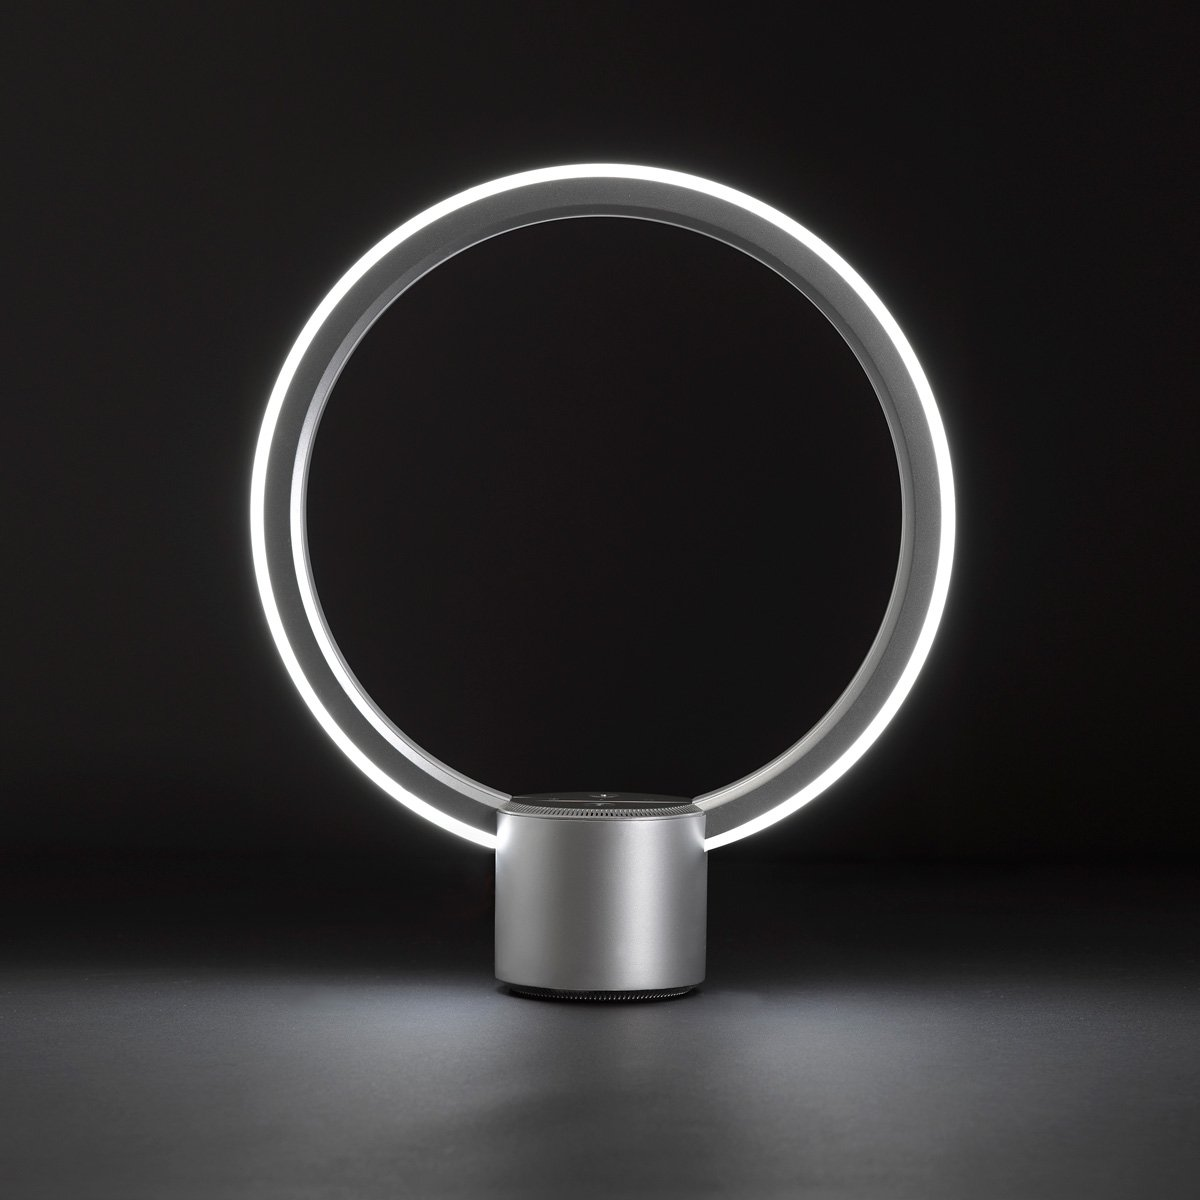
\includegraphics[scale=0.2]{sol1.jpg}
\caption{C by GE Sol, an intelligent lamp bed using Amazon Alextra.}
\label{fig:c}
\end{figure}

\subsubsection{Philips wake-up lamps}
Philips has created a broad range of wake-up lamps designed to impact the sleep-wake cycle of the users. \Cref{fig:philips1,fig:philips2} are examples of the recent versions of Philips' clocks able to simulate sunrise and sunset which last from 20 to 40 mm. These simulations vary the colour of the light following the sun's natural sunrise colour and end with a selected channel or prefered user's music. These Sleep and Wake-up lights are the only wake-up lamp clinically proven to work as stated by Philips\cite{philips}. 

\begin{figure}[h!]
\centering
\begin{minipage}[b]{0.45\textwidth}
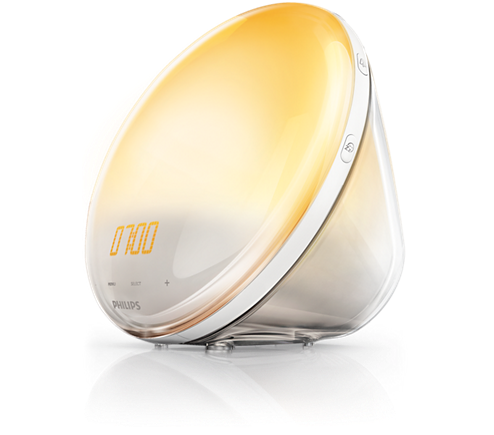
\includegraphics[scale=0.4]{philips1.png}
\subcaption[first caption.]{HF3531/60, coloured sunrise\\ simulation, 7 natural sounds, Tap\\ snooze and reading lamp, midnight\\ light function}
\label{fig:philips1}
\end{minipage}
\begin{minipage}[b]{0.45\textwidth}
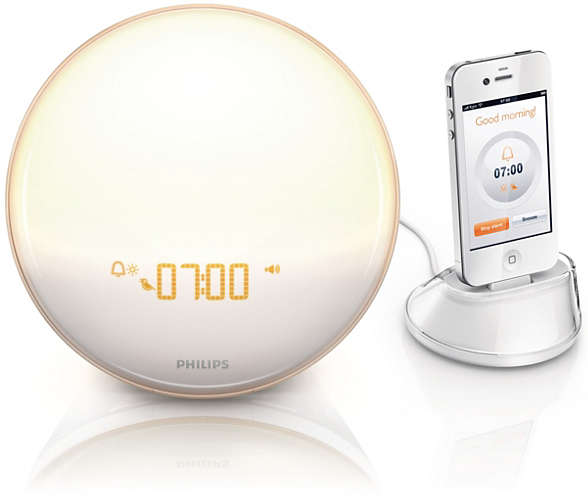
\includegraphics[scale=0.35]{philips2.jpeg}
\subcaption[second caption.]{HF3551/60, coloured sunrise simulation, 7 natural sounds, Tap snooze and reading lamp, midnight light function, Operated by iPhone App}
\label{fig:philips2}
\end{minipage}
\caption{Wake-up light by Philips}
\label{philips}
\end{figure}

\vfill
NEED SOME TRANSITION HERE 

%%%%%%%%%%%%%%%%%%%%%%%%%%%%%%%%%%%%%%%%%%%%%%%%%%%%%%%%%%%%%%%%%%%%%%%%%%%%%%%%%%%%
% SECTION: Hardware modules 
%%%%%%%%%%%%%%%%%%%%%%%%%%%%%%%%%%%%%%%%%%%%%%%%%%%%%%%%%%%%%%%%%%%%%%%%%%%%%%%%%%%%
\section{Hardware modules}
This section provides the research on the hardware technologies as well as the reasons behind the choice of some of these technologies. 

\subsection{Processors and microcontrollers}
A microcontroller is an integrated circuit which is dedicated to execute tasks of a specific application. It is physically small, cheap compared to a computer, and is designed to operate a low power consumption \cite{ho2000}.\\
Numerous microcontrollers were analysed for this project. Each manufacturer provides various range of microcontroller suitable for different applications.
The NPSC's microcontroller needs to communicate to a smartphone application wirelessly and control various external modules. While controlling the external modules, the microcontroller needs to perform processing of the sunrise and sunset patterns by continuously organising and sending data to the neopixels. In order to reduce the complexity of finding the \textit{perfect} microcontroller for the NPSC, the selection was based on the following characteristics:
\begin{itemize}
\item \textbf{Size of the FLASH:} How many lines of code can be loaded to the microcontroller?
\item \textbf{Cost}
\item \textbf{Clock speed}
\item \textbf{Community:} Does the manufacturer have a large community of developers?
\item \textbf{Bit precision:} Are we aiming at 8, 16, or 32 bits precision? 
\item \textbf{Familiarity:} How familiar are we with the microcontroller (time is a constraint)?
\item \textbf{Number of pins:} How many ports does it provide?\
\item \textbf{Extra features:} What are the built-in functionalities (wifi module, bluetooth)?
\end{itemize}

\Cref{table:micro} provides the difference between the microcontrollers selected, this table was use to make the final decision on the microcontroller selection.
\begin{table}[h!]
\centering
\begin{tabular}{cp{5em}p{8em}p{5em}c}
\hline
\hline
\multirow{2}{*}{Characteristics}  & \multicolumn{4}{c}{Microcontrollers} \\  
 & \textbf{Arduino Due} & \textbf{Intel Edison} & \textbf{Raspberry Pi Zero} & \textbf{STM32F407VGT6} \\
\hline
\textbf{Clock speed} & 84MHz &  dual-core, dual-threaded 500 MHz CPU & 1GHz single core & 168 MHz\\
\textbf{Bit precision} & 32 & 32 & 32 & 32 \\
\textbf{FLASH} & 512KB & 4GB & MicroSDHC & 1MB \\
\textbf{Pins} & 54 & 40 & 40 & 82\\
\textbf{Cost} & R549.25 & R687.87 & R79.8 & R114.83\\
\hline
\hline
\end{tabular}
\caption{Comparison between specifications of the Arduino Due \cite{arduino}, the Intel Edison \cite{intel}, the Raspverry Pi Zero \cite{raspberry}, and the STM32F407VGT6\cite{stm}}
\label{table:micro}
\end{table}

\subsection{Storage}
Storages are important in the development of embedded solutions. The \textbf{Electrical Erasable Programmable Read-Only Memory} (EEPROM) is a non-volatile memory capable of keeping its data after being powered off. There are two types of EEPROMs, serial and parallel EEPROMs. In a study made by Microship on the difference between serial and parallel EEPROM of 16KB, Tom Tyson from the Memory Product Divisions concluded that the serial EEPROM is \textit{the best option for embedded solutions requiring a small EEPROM footprint, low current and low operating voltage, the ability and ease to programme a byte at a time, and the best price-performance non-volatile memory solution available}\cite{serialvsparallel} (pp. 4).
The NPSC needs to store the user's data and the NPSC default's settings. Having a non-volatile external memory easy to program is of benefits to the NPSC.

\subsection{Wireless technology}\label{wireless_technologies}
Different types of wireless technologies allow devices to communicate to each other wirelessly. The Institute of Electrical and Electronics Engineers (IEEE) has grouped them in the 802.15 technologies. Among these are the well-known Wifi, cellular machine to machine (M2M), mesh network using ZigBee, Z-wave \ldots and Bluetooth. \\
The NPSC needs to make a wireless connection to communicate with a smartphone application. The appropriateness of the technologies tabulated in \cref{tab:wireless} for the NPSC are analysed below. 
Wifi modules are inexpensive; however, smartphones communicating with the NPSC will require being connected to the same wifi. Moreover, a web application might need to be designed as a platform for the NPSC, this will raise security issues that we would not be able to explore to the time constraint of the project. Cellular machine to machine has one main drawback, its recurring cost. As its name indicate, this technology is to send information from a machine to another machine and is not optimal for a graphic design platform\footnote{having a phone or web application that make use of this would be horrible}.  Mesh networks are optimal for interactions of device/machine of the same kind (not a requirement), the NPSC does not fall into that category. Bluetooth is designed for short-range communication (the typical distance is around $10m$  \footnote{can be increased by increasing the transmission power})being in almost all smartphones it has been extensively used by embedded systems device such as handsets, Bluetooth speakers. It has a full-duplex communication with synchronous and asynchronous channel. Using Bluetooth, the NPSC will not require any network or incur any recurring cost to the user. 

\begin{table}[h!]
\centering
\begin{tabular}{ccc}
\hline
\hline
\textbf{Technology} & \textbf{Constraints} & \textbf{Convenience} \\
\hline
\textbf{Wifi} & Wifi network and security protocol & Yes\\ 
\textbf{M2M} & Recurring cost & No\\
\textbf{Mesh} network & Machine/Device of the same kind & No\\
\textbf{Bluetooth} & Short range & Yes\\
\hline
\hline
\end{tabular}
\caption{Comparison between the constraints and the convenience of Wifi, M2M, Mesh network, and Bluetooth}
\label{table:wireless}
\end{table}

\subsection{Touch screen}
A touch-screen device can locate the position of a point of contact on its screen. 
\Cref{fig:screen} illustrates the difference between resistive and capacitive touchscreen. Resistive touch-screens are made out of many layers of which two are composed of indium-tin-oxide (ITO) which is highly resistive and transparent. By applying pressure on one of the layers, the layers come in contact creating a signal that is used to find the location of the point of contact. Capacitive touch-screens, on the other hand, make use of the conductivity of the object in contact with the screen to affect the electrostatic field between the ITO layers. Resistive touch-screens are less complex than capacitive touch-screens, thus cheaper. Additionally, because they rely on pressure, any object whether conductive or not can be used on the screen which is made to be robust. However, resistive touch-screens do not support multi-touch and have poor contrast because of the extra layer used to protect the ITO layers.\\
The NPSC need to have an onboard controller. This controller must be user-friendly, with the different features of the NPSC, a touch-screen is desirable over a controller with physical buttons. A resistive touchscreen would add to the robustness of the NPSC as a whole.   
\begin{figure}[h!]
\centering
\begin{minipage}[b]{0.45\textwidth}
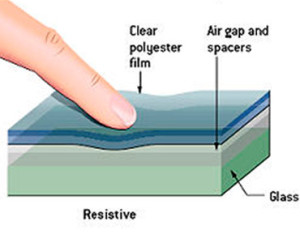
\includegraphics[scale=0.4]{resistiveTouch.jpg}
\subcaption[first caption.]{Resistive touch-screen technology\cite{resistivetouch}.}
\label{fig:resistive_screen}
\end{minipage}
\begin{minipage}[b]{0.45\textwidth}
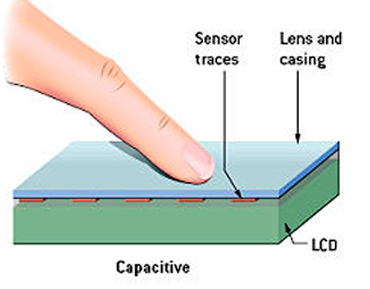
\includegraphics[scale=0.35]{capacitiveTouch.jpg}
\subcaption[second caption.]{Resistive touch-screen technology \cite{capacitivetouch}.}
\label{fig:capacitive_screen}
\end{minipage}
\caption{Touch-screen technologies. More pressure need to be applied on the resistive touch screen for location dectection.}
\label{fig:screen}
\end{figure}    

\subsection{Neopixels}\label{neopixels}
The neopixel is a programmable light source using an MCU to control an RGB or RGBW LEDs. Each colour is capable of producing 255 brightness levels resulting in 16777216 different RGB colours. 
The light characteristics of the neopixel of choice are presented in \cref{table:neopixel_specs}. The light requirement of the NPSC is the emmission of light of $460nm$ (blue light) at an illuminance of $30lux$ minimum.
\begin{table}[h!]
\centering
\begin{tabular}{cp{6em}p{6em}p{6em}}
\hline
\hline
\textbf{Emitting colour} & \textbf{Wavelength (nm)} & \textbf{Luminous intensity (mcd)} & \textbf{Colour temperature (K)} \\ 
\hline
\textbf{Red} & 620-630 & 390-420 & N/A\\
\textbf{Green} & 515-525 & 660-720 & N/A  \\
\textbf{Blue} & 460-470 & 180-200 & N/A\\
\textbf{Natural White} & N/A & N/A & 4000-4500\\
\hline
\hline
\end{tabular}
\caption{Light specification of the SK6812RGBW neopixels}
\label{table:neopixel_specs}
\end{table}
The illuminance of a light source at a point is given by: 
\begin{equation}\label{eq:illuminance}
E_{v(lx)}=\frac{I_{v(cd)}}{d_m^2}
\end{equation}
\cref{eq:illuminance} is the illuminance directly in front of the light source. \textbf{Lambert's Cosine Law} says that the illuminance \textit{is directly proportional to the cosine of the angle made by the normal to the illuminated surface with the direction of the incident flux.} \cite{optical}, mathematically it means:
\begin{equation}\label{eq:lambert}
E_{v_1}=E_v*\cos(\theta)
\end{equation}
\textit{with $\theta$, the angle θ between the direction of the incident light and the surface normal}.\\
The dimension to be considered for the calculation of the illuminance of the neopixel ring are shown in \cref{fig:neopixel_ring_dimension}.
\begin{figure}[h!]
\centering
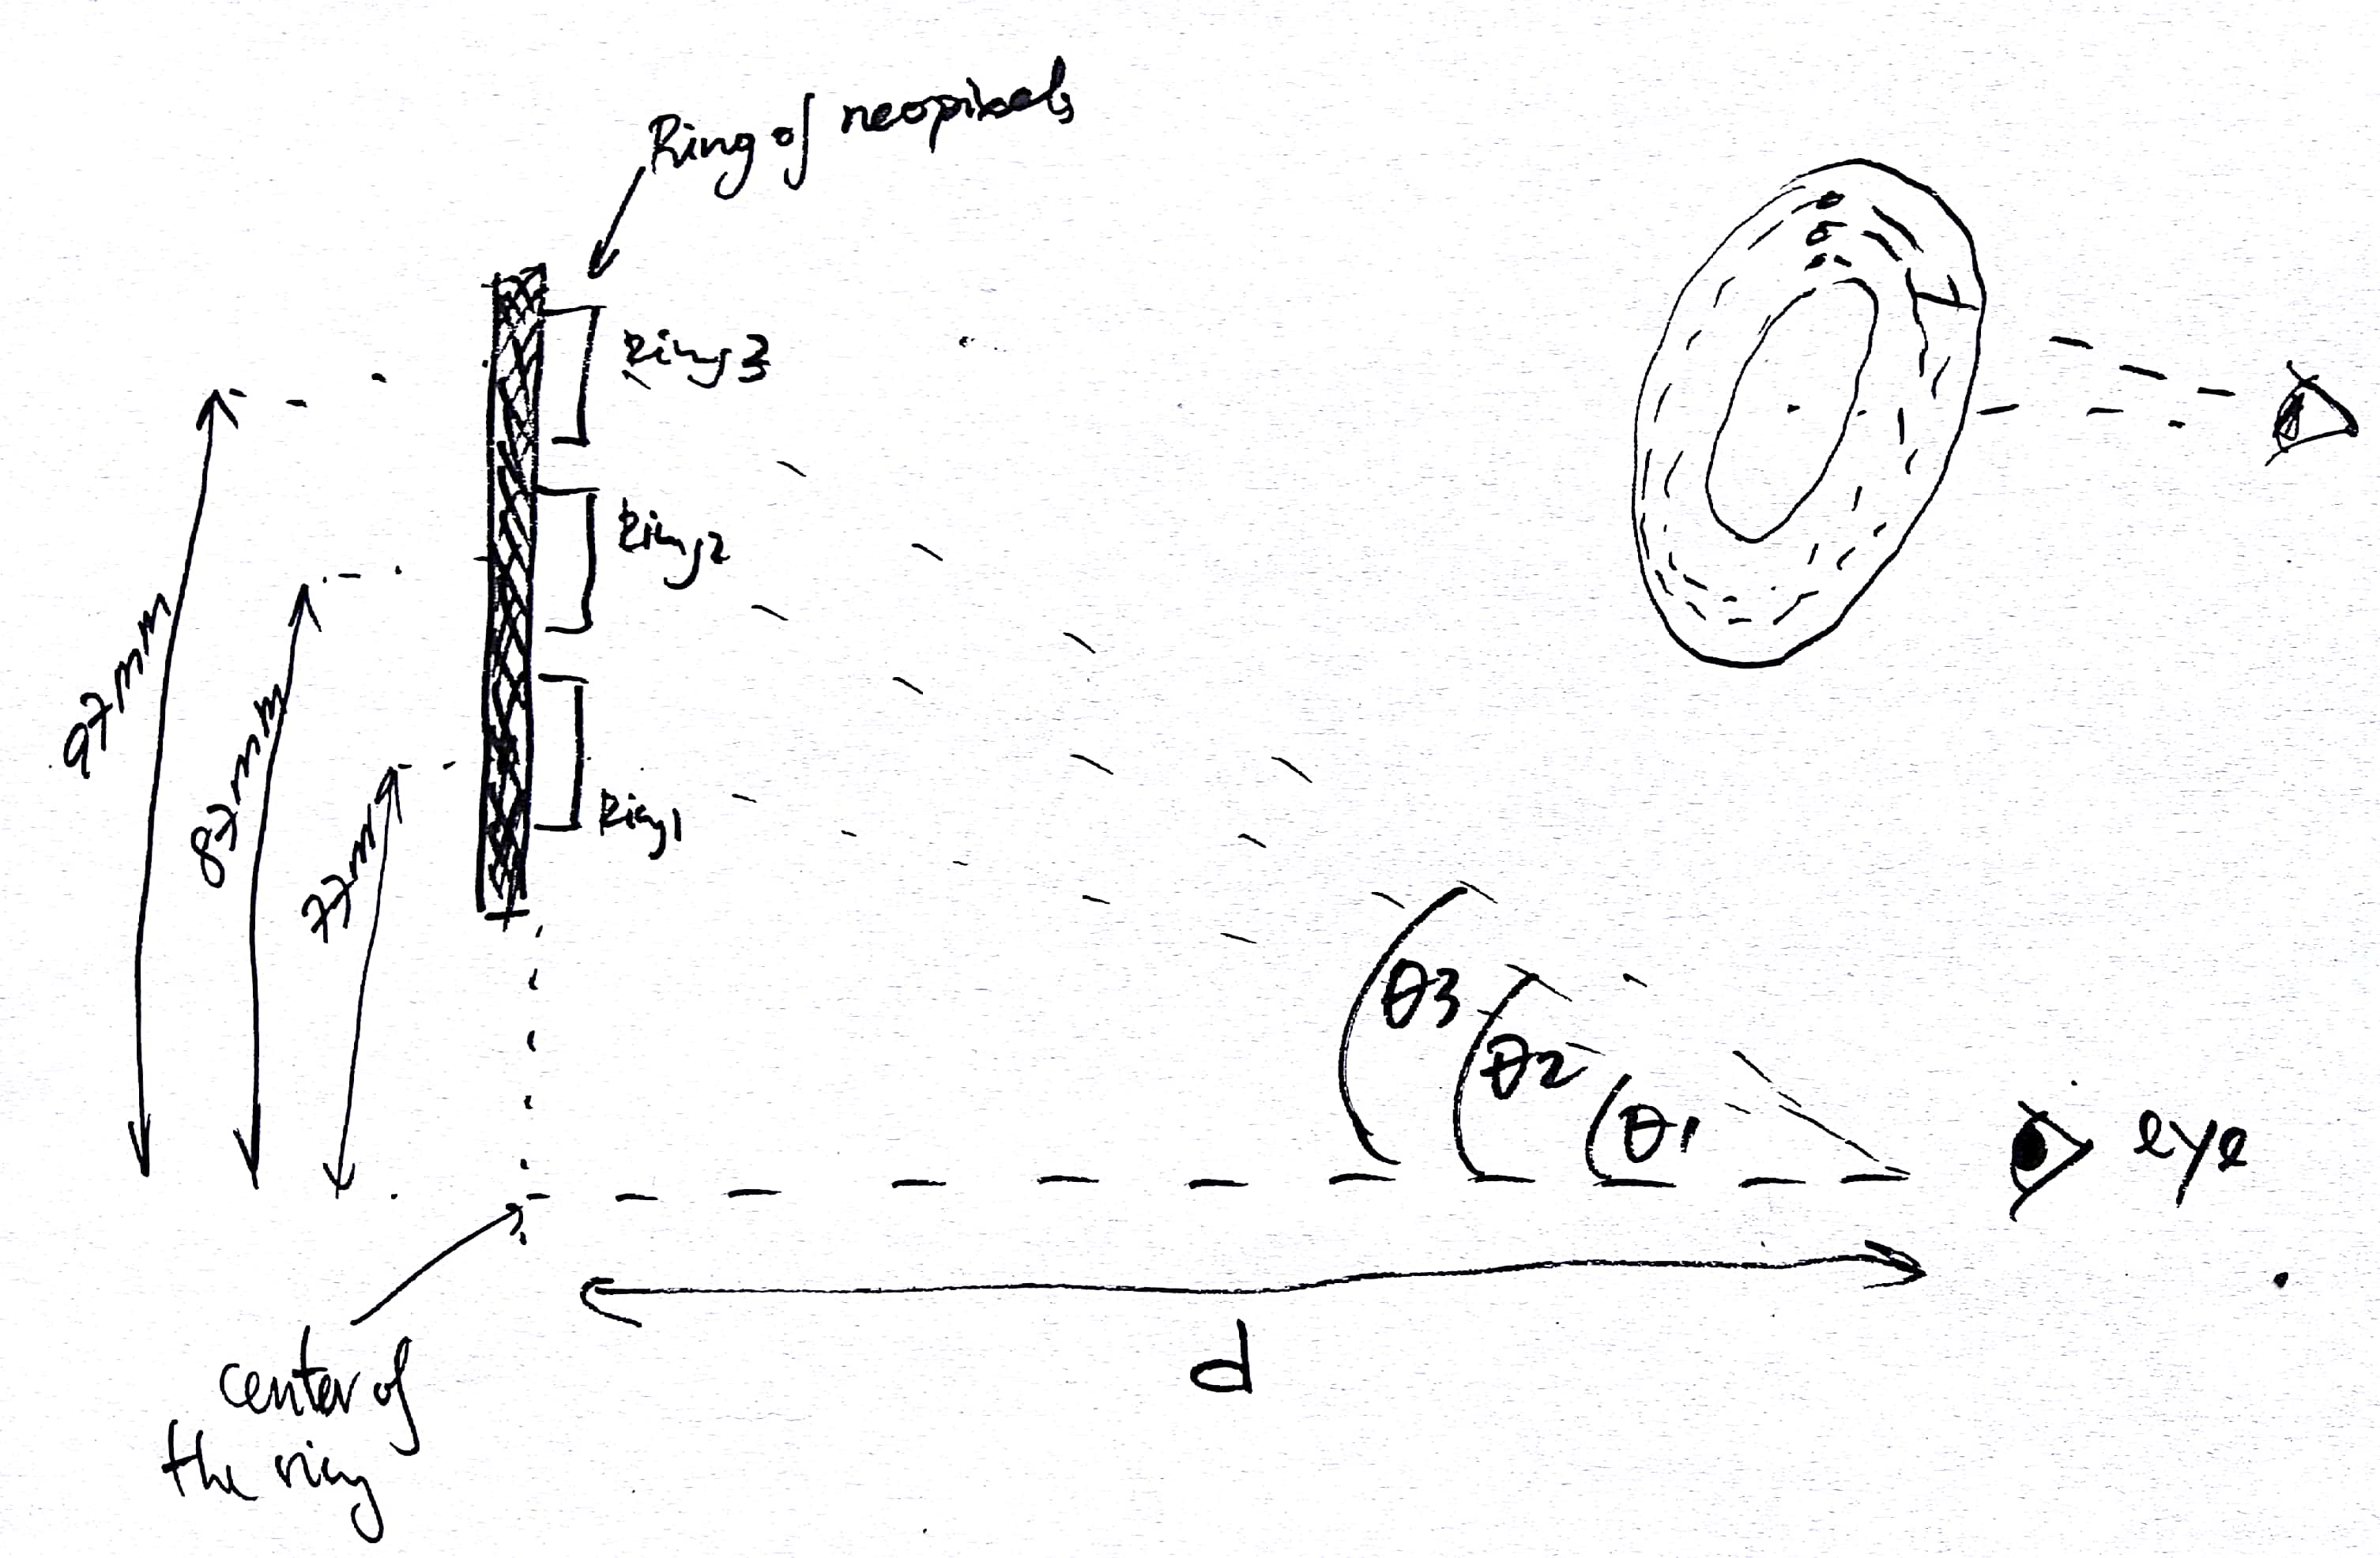
\includegraphics[scale=0.1]{ring_calculation.jpg}
\caption{Relative position of the neopixel rings}
\label{fig:neopixel_ring_dimension}
\end{figure}
Using the dimension from \cref{fig:neopixel_ring_dimension} and the intensity from \cref{table:neopixel_specs} for the blue light, the total illuminace of the rings at a specific distance can be calculated using the following equation:
\begin{equation}\label{eq:total_illuminance}
E_{v_{total}} = N*Ev*(\cos(\theta_1)+\cos(\theta_2)+\cos(\theta_3))
\end{equation}
The result of the calculation are tabulated in the \cref{neopixel_illuminance}. The NPSC will not meet the light requirement if the it is placed more than one meter away from the subject.
\begin{table}[h!]
\centering
\begin{tabular}{ccc}
\hline
\hline
\multirow{2}{*}{Distance (cm)}  & \multicolumn{2}{c}{Illuminance (lux)} \\  
 & no angle consideration & with angle \\
\hline
30 & 360 & 345.62\\
40 & 202.5 & 197.82\\
50 & 129.6 & 127.66\\
60 & 90 & 89.06\\
70 & 66.12 & 65.61\\
80 & 50.63 & 50.32\\
90 & 40 & 39.81\\
100 & 32.4 & 32.28\\
110 & 26.78 & 26.69\\
\hline
\hline
\end{tabular}
\caption{Illuminance of the neopixel ring for distance ranging from 30cm to 110cm}
\label{table:neopixel_illuminance}
\end{table}
%%%%%%%%%%%%%%%%%%%%%%%%%%%%%%%%%%%%%%%%%%%%%%%%%%%%%%%%%%%%%%%%%%%%%%%%%%%%%%%%%%%%
% SECTION: Communication protocols
%%%%%%%%%%%%%%%%%%%%%%%%%%%%%%%%%%%%%%%%%%%%%%%%%%%%%%%%%%%%%%%%%%%%%%%%%%%%%%%%%%%%
\section{Communication protocols}
The NPSC requires different integrated circuits using various communication protocols, below is a brief on the use of the protocol required.

\subsection{Serial Peripheral Interface (SPI) Bus}
SPI is a synchronous full duplex serial communication protocol used for short distance communication of electronic devices. With the protocol, one master can communicate to many slaves using a chip select pin (use to select the slave) but a slave can only talk to the master device. SPI uses 4 signals namely, the Master Out Slave In (MOSI), the Master In Slave Out (MISO), the clock (SCK), and the slave select or chip select (SS). Since SPI uses a clock, it does not require the configuration of a baud rate before communication. The main inconvenience with SPI is the number of pins required for a one to one communication, for every additional slave, the master must provide an SS pins which make SPI not the ideal protocol for communicating to multiple slaves devices \cite{spi}. 
\begin{figure}[h!]
\centering
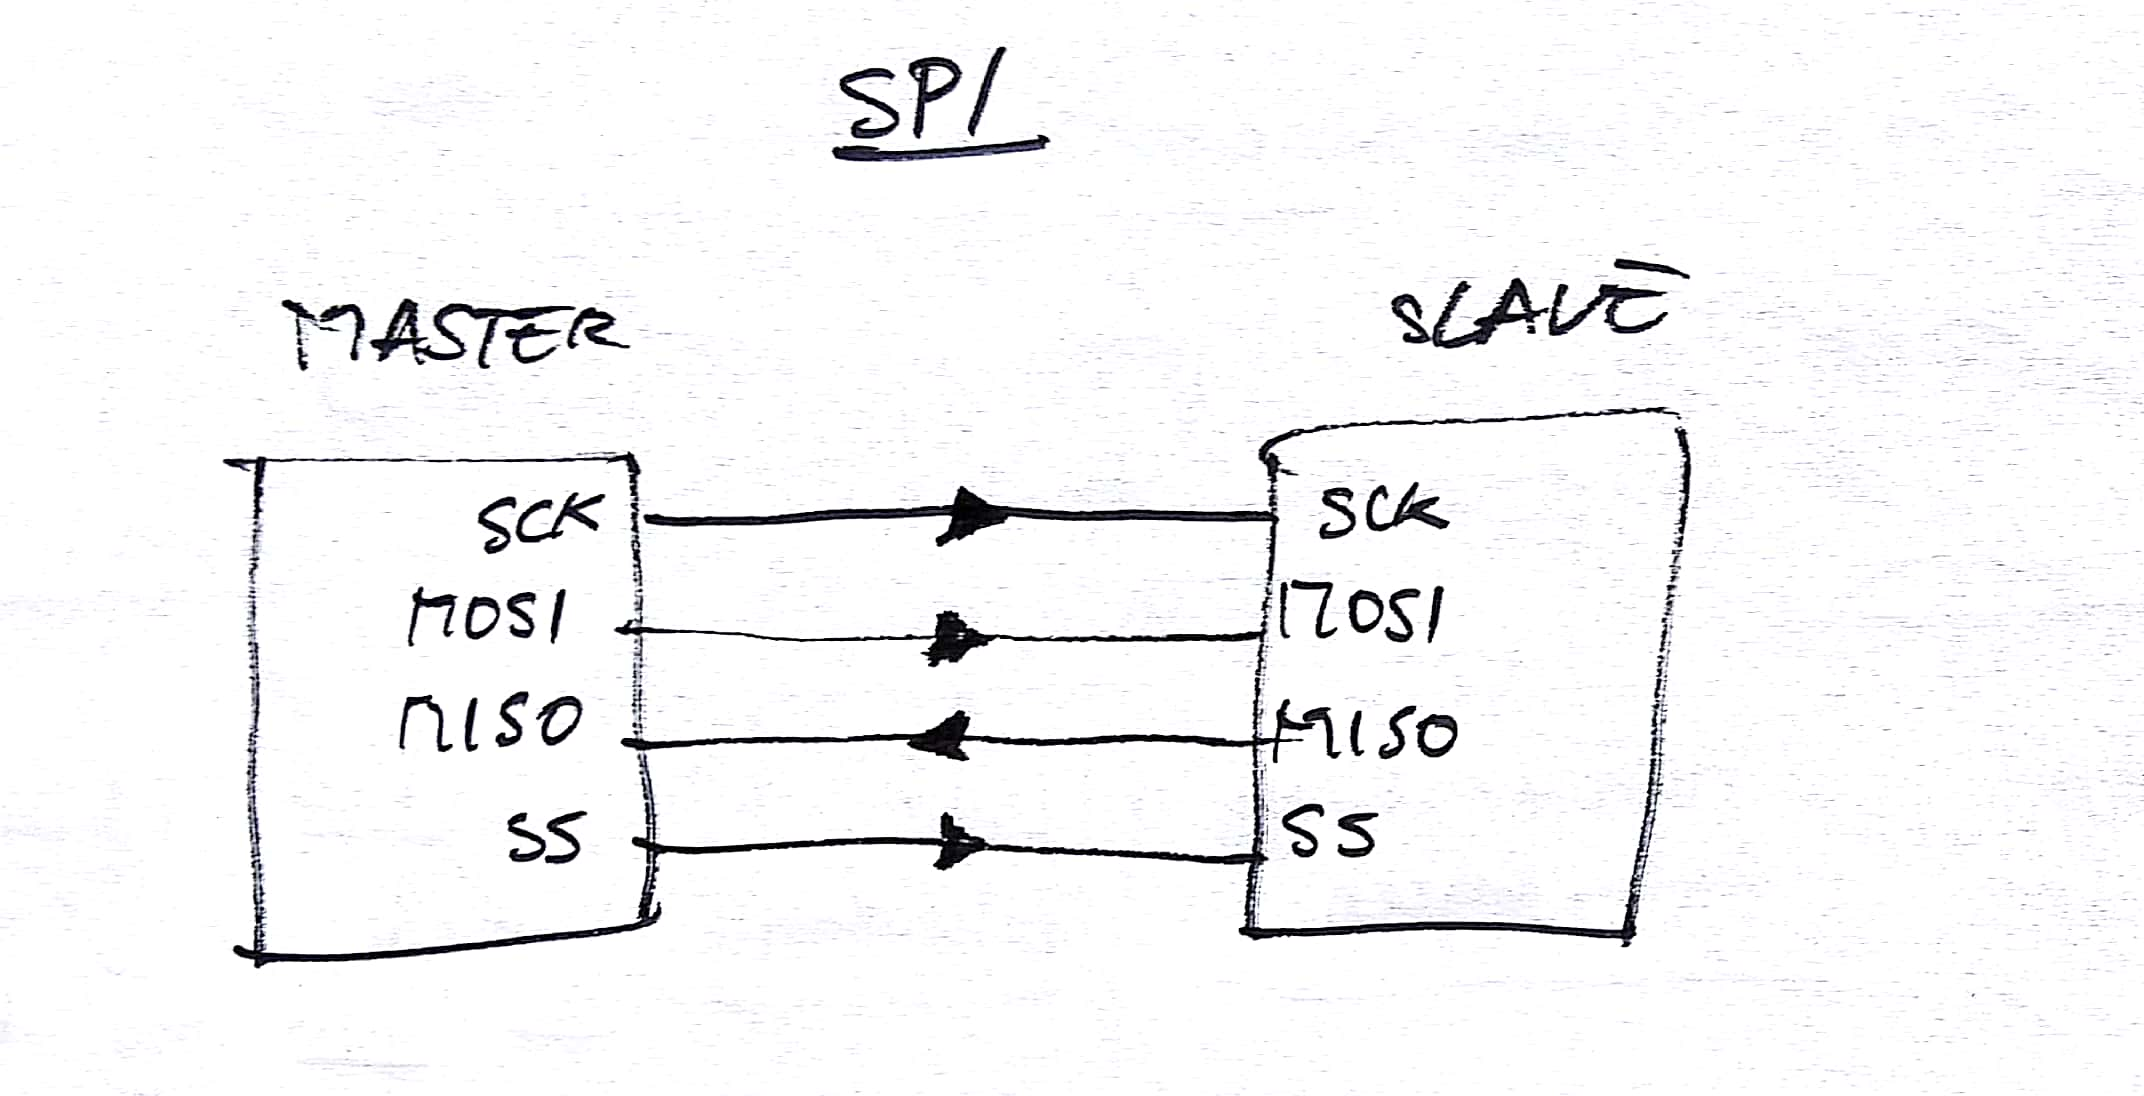
\includegraphics[scale=0.2]{spi.jpg}
\caption{Wire connection setting for SPI communication between a master and a slave device}
\label{fig:spi_coms}
\end{figure}
\subsection{Universal asynchronous receiver-transmitter (UART)}
UART is an asynchronous full duplex communication protocol making use of two signals a transmit signal (TX) and a receive signal (RX). With UART, both devices need to agree on a baud-rate for communication, this rate defines the number of bytes to be sent and received. The problem with UART is the complexity of the protocol required to ensure synchronous communication and correct transfer of information between device. Although theoretically, UART baud-rate is infinite, it is practically limited to 230400 bits per seconds \cite{uart}.   
\begin{figure}[h!]
\centering
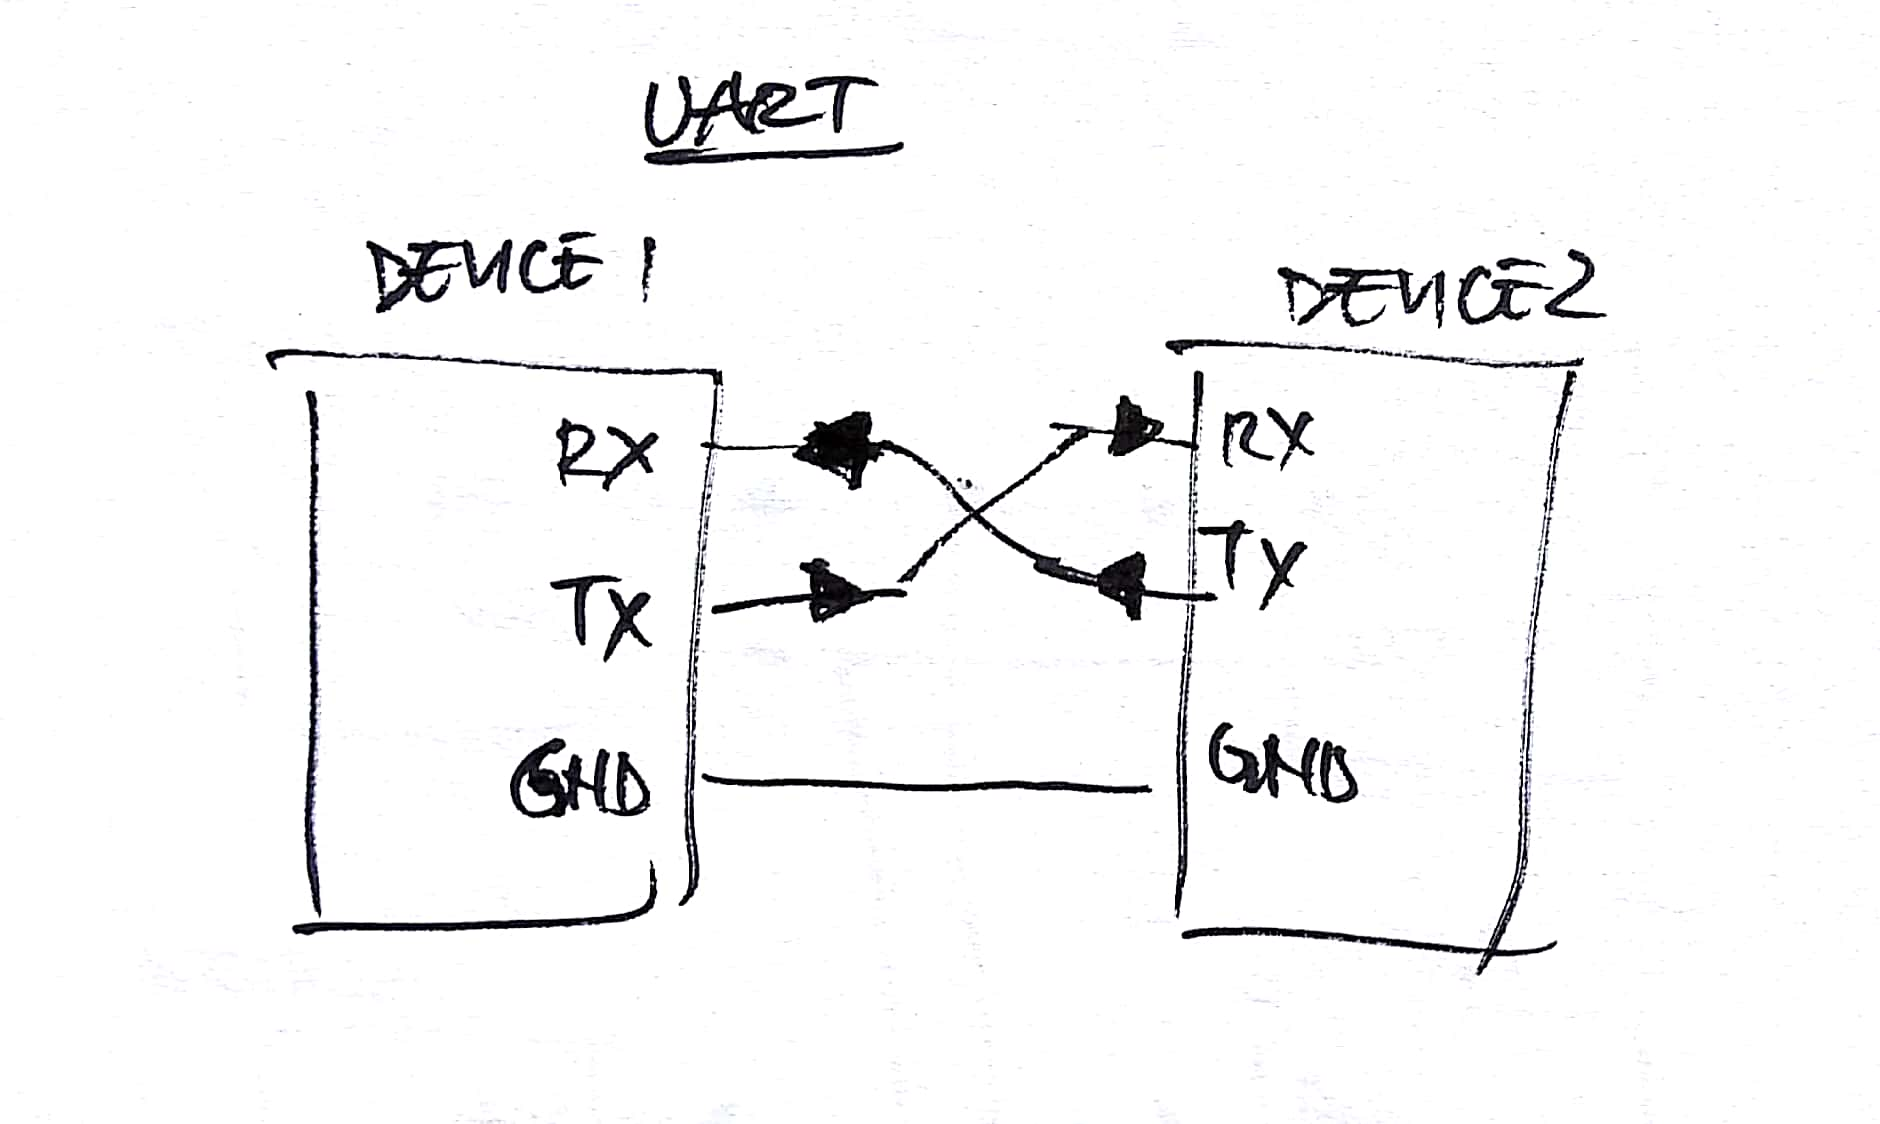
\includegraphics[scale=0.2]{uart.jpg}
\caption{Wire connection setting for UART communication between two devices}
\label{fig:uart_coms}
\end{figure}
\subsection{Inter-Integrated Circuit (I2C)}
I2C is a serial protocol that allows communications from multiple slaves to multiple masters. It takes a bit of both SPI and UART by being designed for short distance communication and requiring only two pins, namely the data line (SDA) and clock line (SCL). Its clock ranges from $100kHz$ to $400kHz$ and a byte is sent at a time. Furthermore, with the I2C protocol, each slave must have a unique address used by the master for communication \cite{i2c}.  
\begin{figure}[h!]
\centering
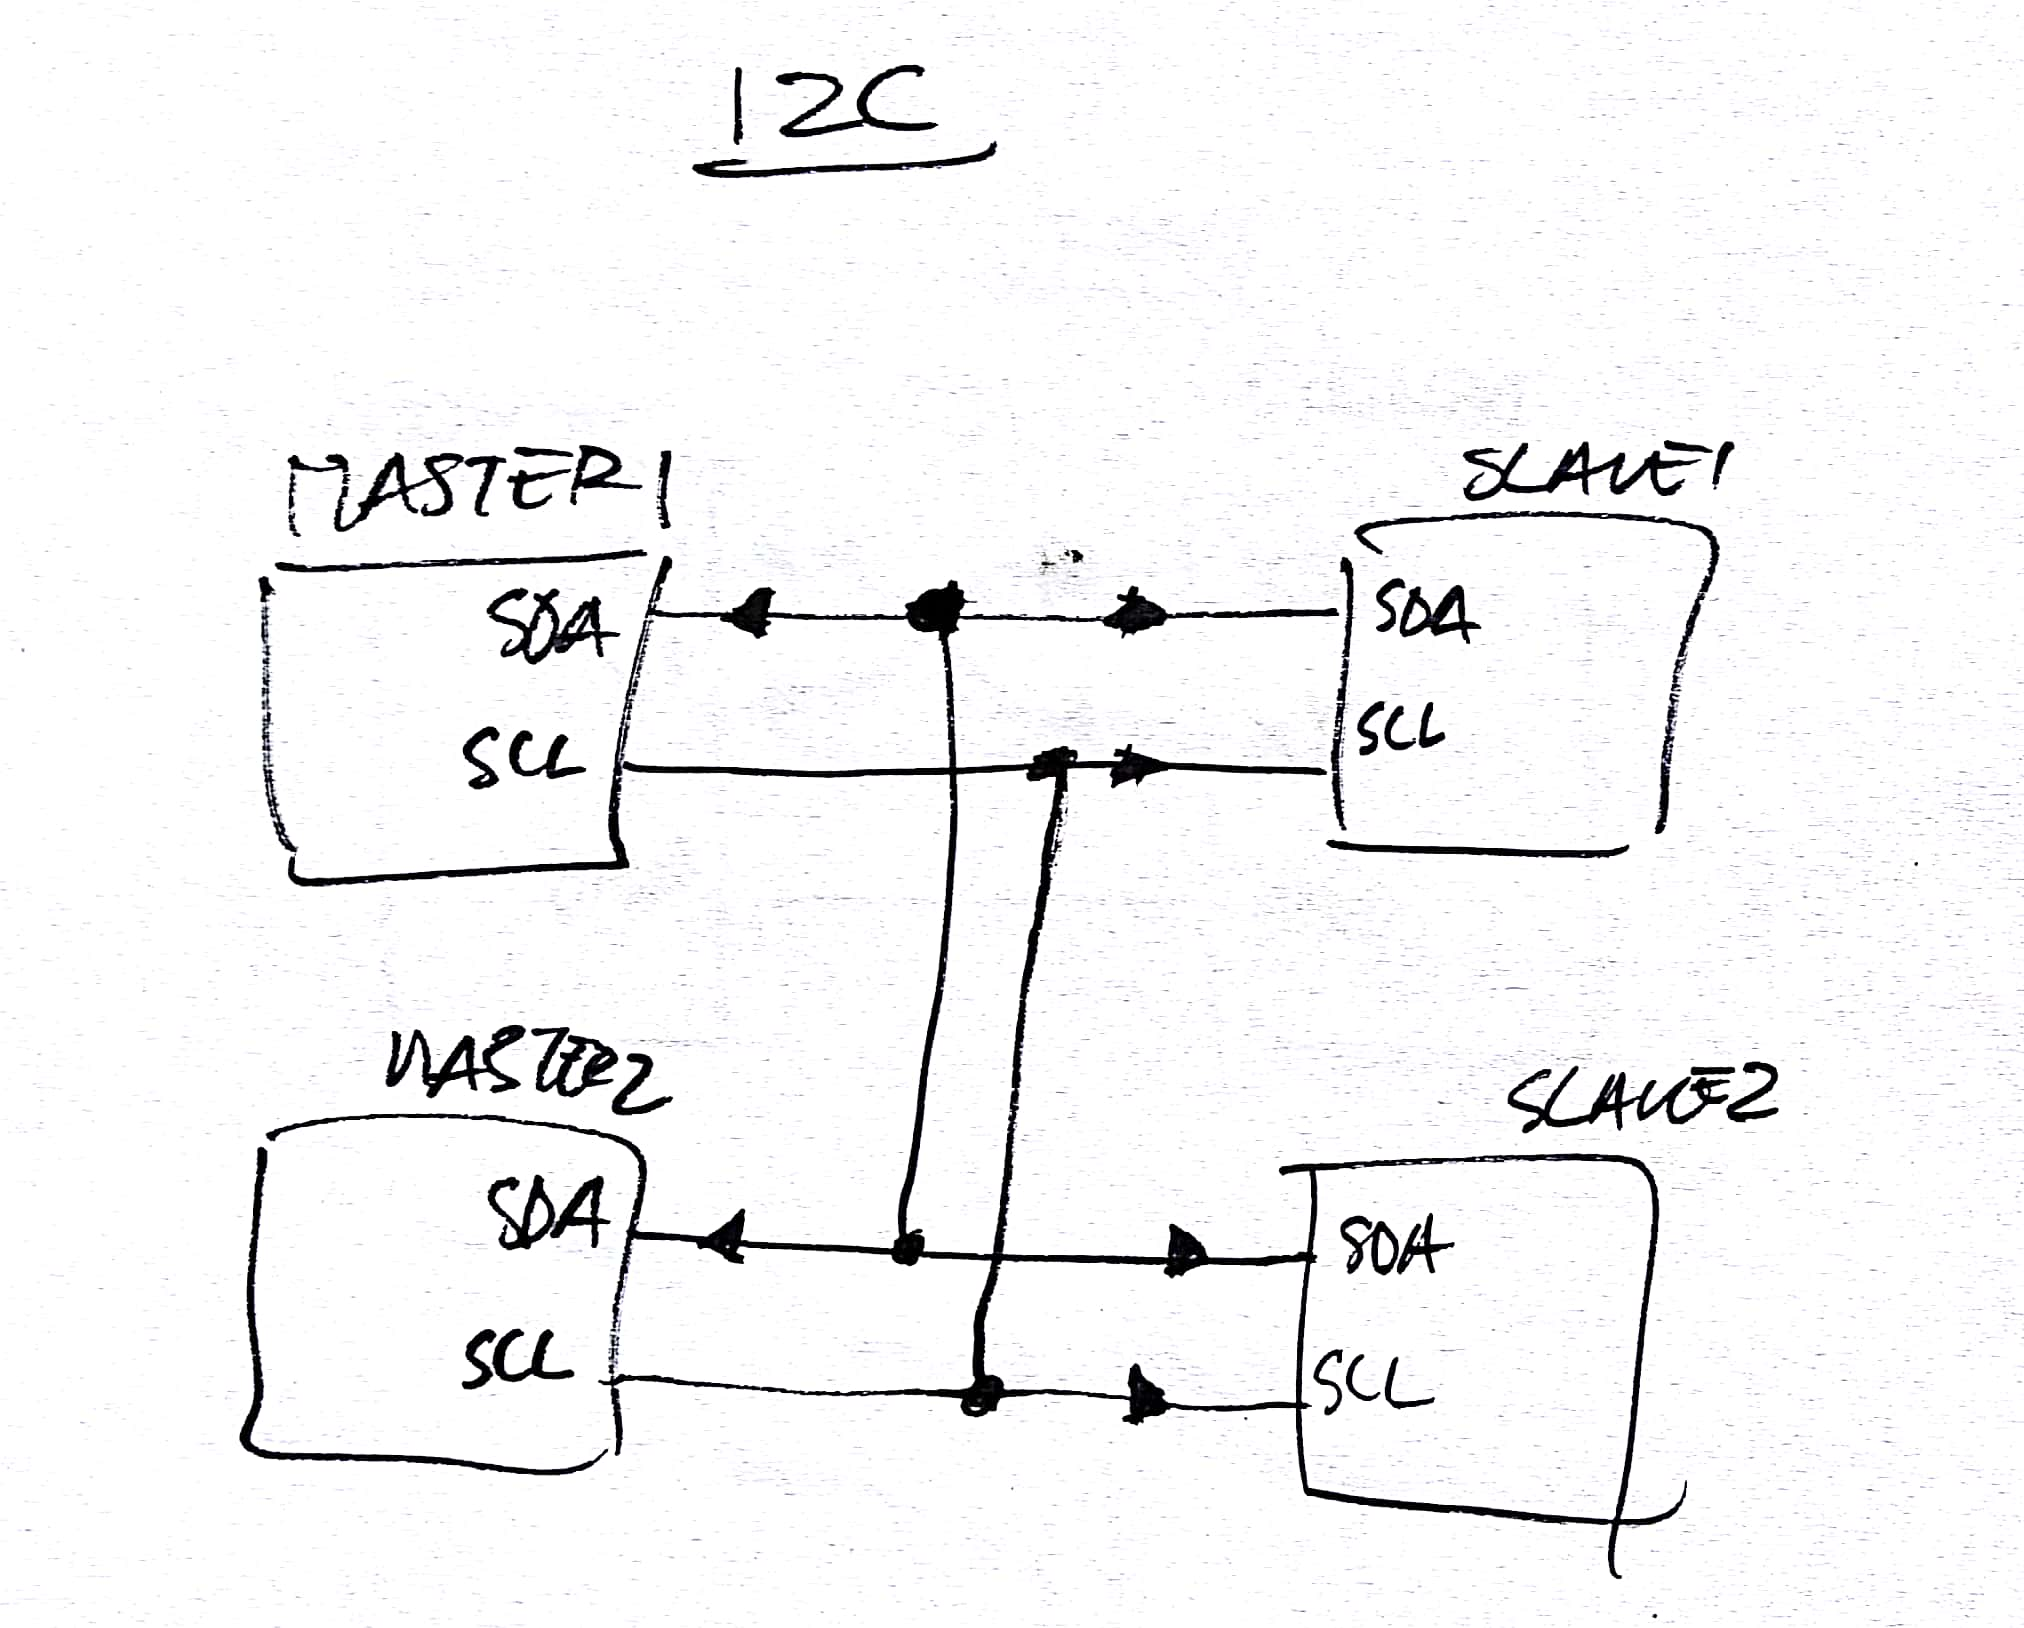
\includegraphics[scale=0.2]{i2c.jpg}
\caption{Wire connection setting for I2C communication between two masters and two slaves devices}
\label{fig:i2c_coms}
\end{figure}
\subsection{Neopixels serial protocol}
Each neopixel has a built-in IC controlling the LEDs' intensity based on the data received. The neopixels use a single wire communication protocol. The neopixels can be connected to form a daisy chain (cascade)\cref{fig:neopixel_cascade} allowing to program of a series of neopixels using one signal. Each neopixel requires 24 Bytes (32 Bytes for RGBW LEDs), each bytes is an encoded bit using a Non-Return-to-Zero encoding \cref{fig:neopixel_nrz}. On receiving a sequence of data, the first neopixel in the chain takes the first 24 bytes and passes the rest of the data to the next neopixel in the daisy chain and so for. This operation continues until a \textit{rest signal} is received by the first neopixel \cref{fig:neopixel_cascade}. This is possible because each neopixel is capable of reshaping the incoming signal preserving the integrity its integrity of continuous transmission.

\begin{figure}[h!]
\centering
\begin{minipage}[b]{0.45\textwidth}
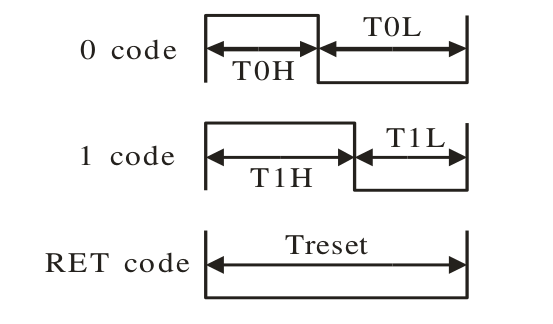
\includegraphics[scale=0.4]{neopixel_nrz.png}
\subcaption[first caption.]{Non-return-to-zero encoding of a single bit in the neopixels programming protocol}
\label{fig:neopixel_nrz}
\end{minipage}
\begin{minipage}[b]{0.45\textwidth}
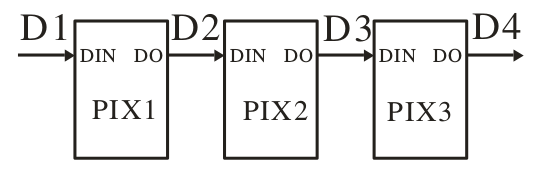
\includegraphics[scale=0.4]{neopixel_cascade.png}
\subcaption[second caption.]{Neopixels connected in daisy chain (cascade).}
\label{fig:neopixel_cascade}
\end{minipage}
\begin{minipage}[b]{\textwidth}
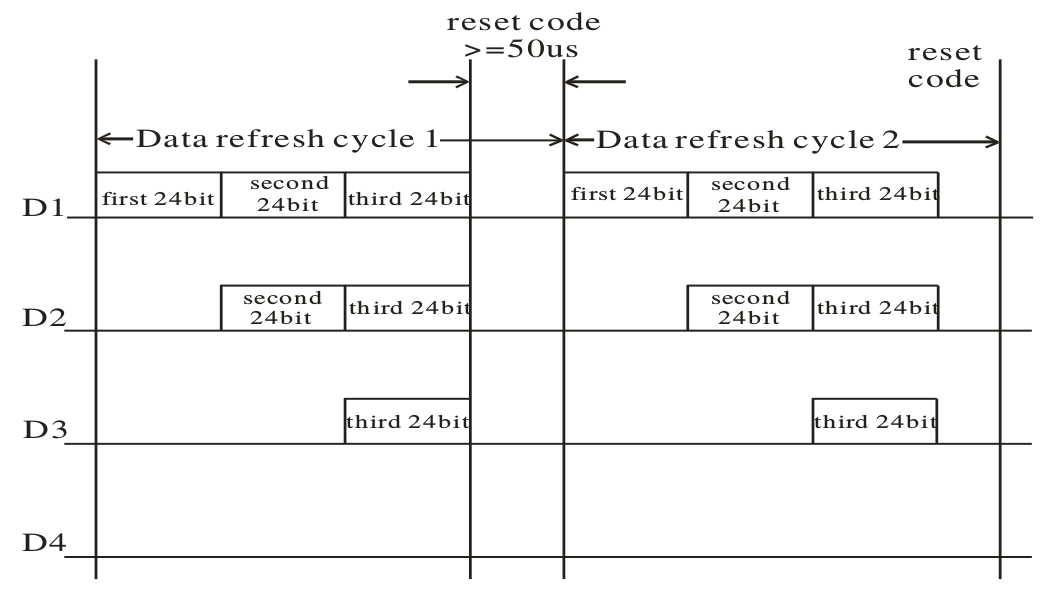
\includegraphics[scale=0.45]{neopixel_serial.png}
\subcaption[third caption.]{As the first neopixel receives a stream of multiple 8 Bytes chunck of data, it takes the first 8 Bytes from the stream and transmit the rest to the next neopixel in the cascade. A rest signal indicates where the stream of data ends.}
\label{fig:neopixel_cascade}
\end{minipage}
\caption{Illustration of the neopixels serial interface}
\label{fig:neopixel_protocol}
\end{figure}
 
%%%%%%%%%%%%%%%%%%%%%%%%%%%%%%%%%%%%%%%%%%%%%%%%%%%%%%%%%%%%%%%%%%%%%%%%%%%%%%%%%%%%
% SECTION: PCB Board Design
%%%%%%%%%%%%%%%%%%%%%%%%%%%%%%%%%%%%%%%%%%%%%%%%%%%%%%%%%%%%%%%%%%%%%%%%%%%%%%%%%%%%
\section{PCB Board Design}\label{PCB_requirement}
Printed Circuit Boards (PCBs) are almost present in every electronic circuit as they hold all the components together and implement the electrical connections. Designing a PCB is a process easily prone to errors, therefore a good PCB design requires the implementation of the design steps. \Cref{fig:pcb_design_flow} illustrates an examples of the ideal pcb design steps. In making the NPSC PCBs these steps give an engineering approach that can be elaborated further based on the PCBs requirement. For example, the designer might question what is the best placement for certain component and thus be referred to some PCBs design standards such as the IPC2221.\\
One important design requirement (need) for the NPSC light requirement is its theoretical current ($10A$) drawn at full pixel brightness. The board-level diagram of the NPSC ring of the neopixel board should therefore be designed so that the track are wide enough to dissipate all the heat evenly across the board. The \textbf{IPC2221}, a generic standard for printed board design published by the \textit{Association Connecting Electronics Industries} \cite{pcb_design} describes a method for finding the mininmal width track given a specific current (see fig 6-4 from the IPC2221 \cite{pcb_design}(pp. 41)). A Javascript program based on the IPC2221 standard can be easily use to determine the track width \cite{pcb_track_width}. This web application use the track cuurent, thickness, temperature rise, ambient temperature and track lenght as input to determine the required track width.      
\begin{figure}[ht]
\centering
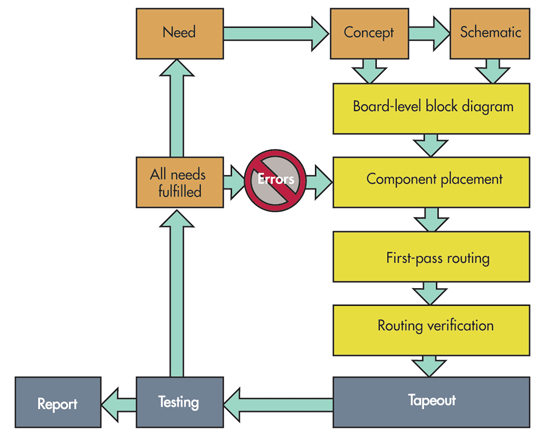
\includegraphics[scale=0.5]{pcb_design_flow.png}
\caption{Ideal PCB design flow, starting from the need, followed by the design, implementation and testing}
\label{fig:pcb_design_flow}
\end{figure}

%%%%%%%%%%%%%%%%%%%%%%%%%%%%%%%%%%%%%%%%%%%%%%%%%%%%%%%%%%%%%%%%%%%%%%%%%%%%%%%%%%%%
% SECTION: Software
%%%%%%%%%%%%%%%%%%%%%%%%%%%%%%%%%%%%%%%%%%%%%%%%%%%%%%%%%%%%%%%%%%%%%%%%%%%%%%%%%%%%
\section{Programming Languages}
Choosing the right programming language for software development is a crutial step, expecially in embedded system design as carefull manipulation of memory is required. The languages below are the ones chosen for the development of NPSC. 
\subsection{C}
\textit{C} is a mid-level programming language \footnote{has the advantages of both ligh and low level language} providing the ability to get close to the hardware while keeping some abstract layers for programming \cite{c_programming}.It has an easy and straight forward syntax compared to languages such as Java, C has accumulated a lot of support and has lots of functions and documentation. Although C does not support Object Orientated Programming, it is a Procedure Orientated Language (POL) which means it is designed to create programs that follow an algorithm. This latter feature of C make it the favourite programming language for Embedded System. 

\subsection{C++}
\textit{C++} is a programming language based on C which has higher level functionality. In the context of this project, C++ is used to test the functionality of the NPSC modules using an Arduino.

%%%%%%%%%%%%%%%%%%%%%%%%%%%%%%%%%%%%%%%%%%%%%%%%%%%%%%%%%%%%%%%%%%%%%%%%%%%%%%%%%%%%
% SECTION: Software Tools and Libraries
%%%%%%%%%%%%%%%%%%%%%%%%%%%%%%%%%%%%%%%%%%%%%%%%%%%%%%%%%%%%%%%%%%%%%%%%%%%%%%%%%%%%
\section{Software Tools and Libraries}
Developing an embedded system software can be quite frustrating, for this reason tools with decent debugging features and programming interface should be chosen to reduce development to its minimal. 

\subsection{Atollic TrueSTUDIO for ARM}
Atollic TrueSTUDIO is an IDE based on Eclipse. It comes with the GCC toolchain for ARM and with debugging features beuilt on top of GDB. It has more advanced features compared to Eclipse in the development embedded system application. Its debugging features include the use of any debug probe compatible with the GDB-server, P\&E Micro, SEGGER J-Link / J-Trace, ST-Link, OpenOCD are all supported by Atollic TrueSTUDIO. It supports debugging of single and multi core devices and allows real time view of memory mapping, peripheral registers, advanced visualisation of variable and complex break point, CPU fault analysis and many more. Another important debugging feature of Atollic TrueSTUDIO is the instruction tracing and system analysis real time event analysis of Real Time Operating System \cite{atollic}.

\subsection{Nextion IDE}\label{nextion}
Nextion IDE is the official IDE designed for programming any Nextion HMI touch-screen. The IDE allows the designed and programmation of a GUI interface and the definition of serial commands to be sent to a MCU. Nextion IDE is designed to reduce significantly development time of touch-screen interface in an embedded system project \cite{nextion}. 

\subsection{MIT App Inventor 2}


%%%%%%%%%%%%%%%%%%%%%%%%%%%%%%%%%%%%%%%%%%%%%%%%%%%%%%%%%%%%%%%%%%%%%%%%%%%%%%%%%%%%
% SECTION: Design Models
%%%%%%%%%%%%%%%%%%%%%%%%%%%%%%%%%%%%%%%%%%%%%%%%%%%%%%%%%%%%%%%%%%%%%%%%%%%%%%%%%%%%
\section{Design Models}
Designing an embedded system requires the use of suitable design methods. This section describes the different design models used for the project.

\subsection{V-Model}
The V-Model is a linear product-development methodology composed of two main parts. On the left side of the diagram (see \cref{fig:v_model} ) is the project definition. On that branch, the requirements are defined, the system design, architectural design and module design are performed. At the bottom of the diagram is the implementation of the design. Following the implementation is the project testing and integration. The project testing starts with the unit testing of the module design followed by integration testing in which the architectural design is tested to ensure that the system functions well across all components. The next step consists of the system testing and the validation of the performance defined in the design. The last step is the acceptance testing, done to ensure that the system can be deployed.       
\begin{figure}[ht]
\centering
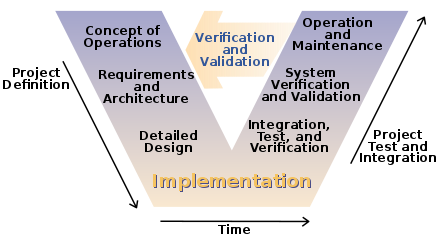
\includegraphics[scale=0.7]{v_model.png}
\caption{V-Model basic template used for system definition and testing}
\label{fig:v_model}
\end{figure}

\subsection{Spiral Model}
The Spiral model is a combination of the iterative model \footnote{Cyclic process consisting of design, prototyping, testing, analysis and refinement of a product} and the waterfall model \footnote{linear sequential process consisting of conception, initiation, analysis, design, construction, testing, deployment and maintenance of a product.} through which a product can be refined after each cycle. \Cref{fig:spiral_model} illustrate the order of the spiral model steps. The first step is the identification, it consists of identifying the user, system, sub-system, and unit requirements. The second step consists of the system, architectural, physical design and logical design of all modules. The prototype is built during the third step, the prototype serves as a proof of concept. During the last stage, the prototype performance is evaluated as well as the validation of the system requirements. Moreover, a risk and cost analysis alongside with the overall feasibility of the project is evaluated at this stage.  
\begin{figure}[ht]
\centering
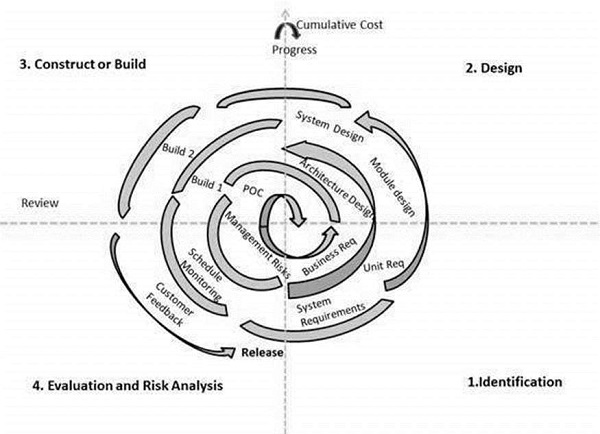
\includegraphics[scale=0.7]{spiral_model.jpg}
\caption{Spiral-Model basic template used for system refinement}
\label{fig:spiral_model}
\end{figure}
\chapter{Prototype Design}
This chapter focuses on the design of the prototype of the NeoPixel Sunrise Clock (NPSC). It starts by providing an overview of the NPSC system design, followed by a high-level description of the sub-systems design and a detailed design of the hardware modules. The system design provides an overview of the NPSC's module. The high-level design focuses on the thinking process behind the design of the applications at level 3 of the system hierarchy. The detailed design focuses on the hardware modules at level 1 of the system hierarchy, providing more detailed on the design of the hardware.

%%%%%%%%%%%%%%%%%%%%%%%%%%%%%%%%%%%%%%%%%%%%%%%%%%%%%%%%%%%%%%%%%%%%%%%%%%%%%%%%%%%%
% SECTION: System design
%%%%%%%%%%%%%%%%%%%%%%%%%%%%%%%%%%%%%%%%%%%%%%%%%%%%%%%%%%%%%%%%%%%%%%%%%%%%%%%%%%%%
\section{System design}
The system requirements of the NPSC are the following:
\begin{itemize}
\item The NPSC should be able to emit light and simulate sunrise. 
\item The NPSC should be able to display time and set alarms.
\item The NPSC should be controllable using a touchscreen device.
\end{itemize}
These system requirements are achieved by the functions of the applications at level 3 of system modular hierarchy illustrated in \cref{fig:system_hierarchy}. Each application focuses on one requirement but might involve other requirements, the relations between some hardware modules and their application module are illustrated by \cref{fig:system_overview} and explained below.
\begin{figure}[ht]
\centering
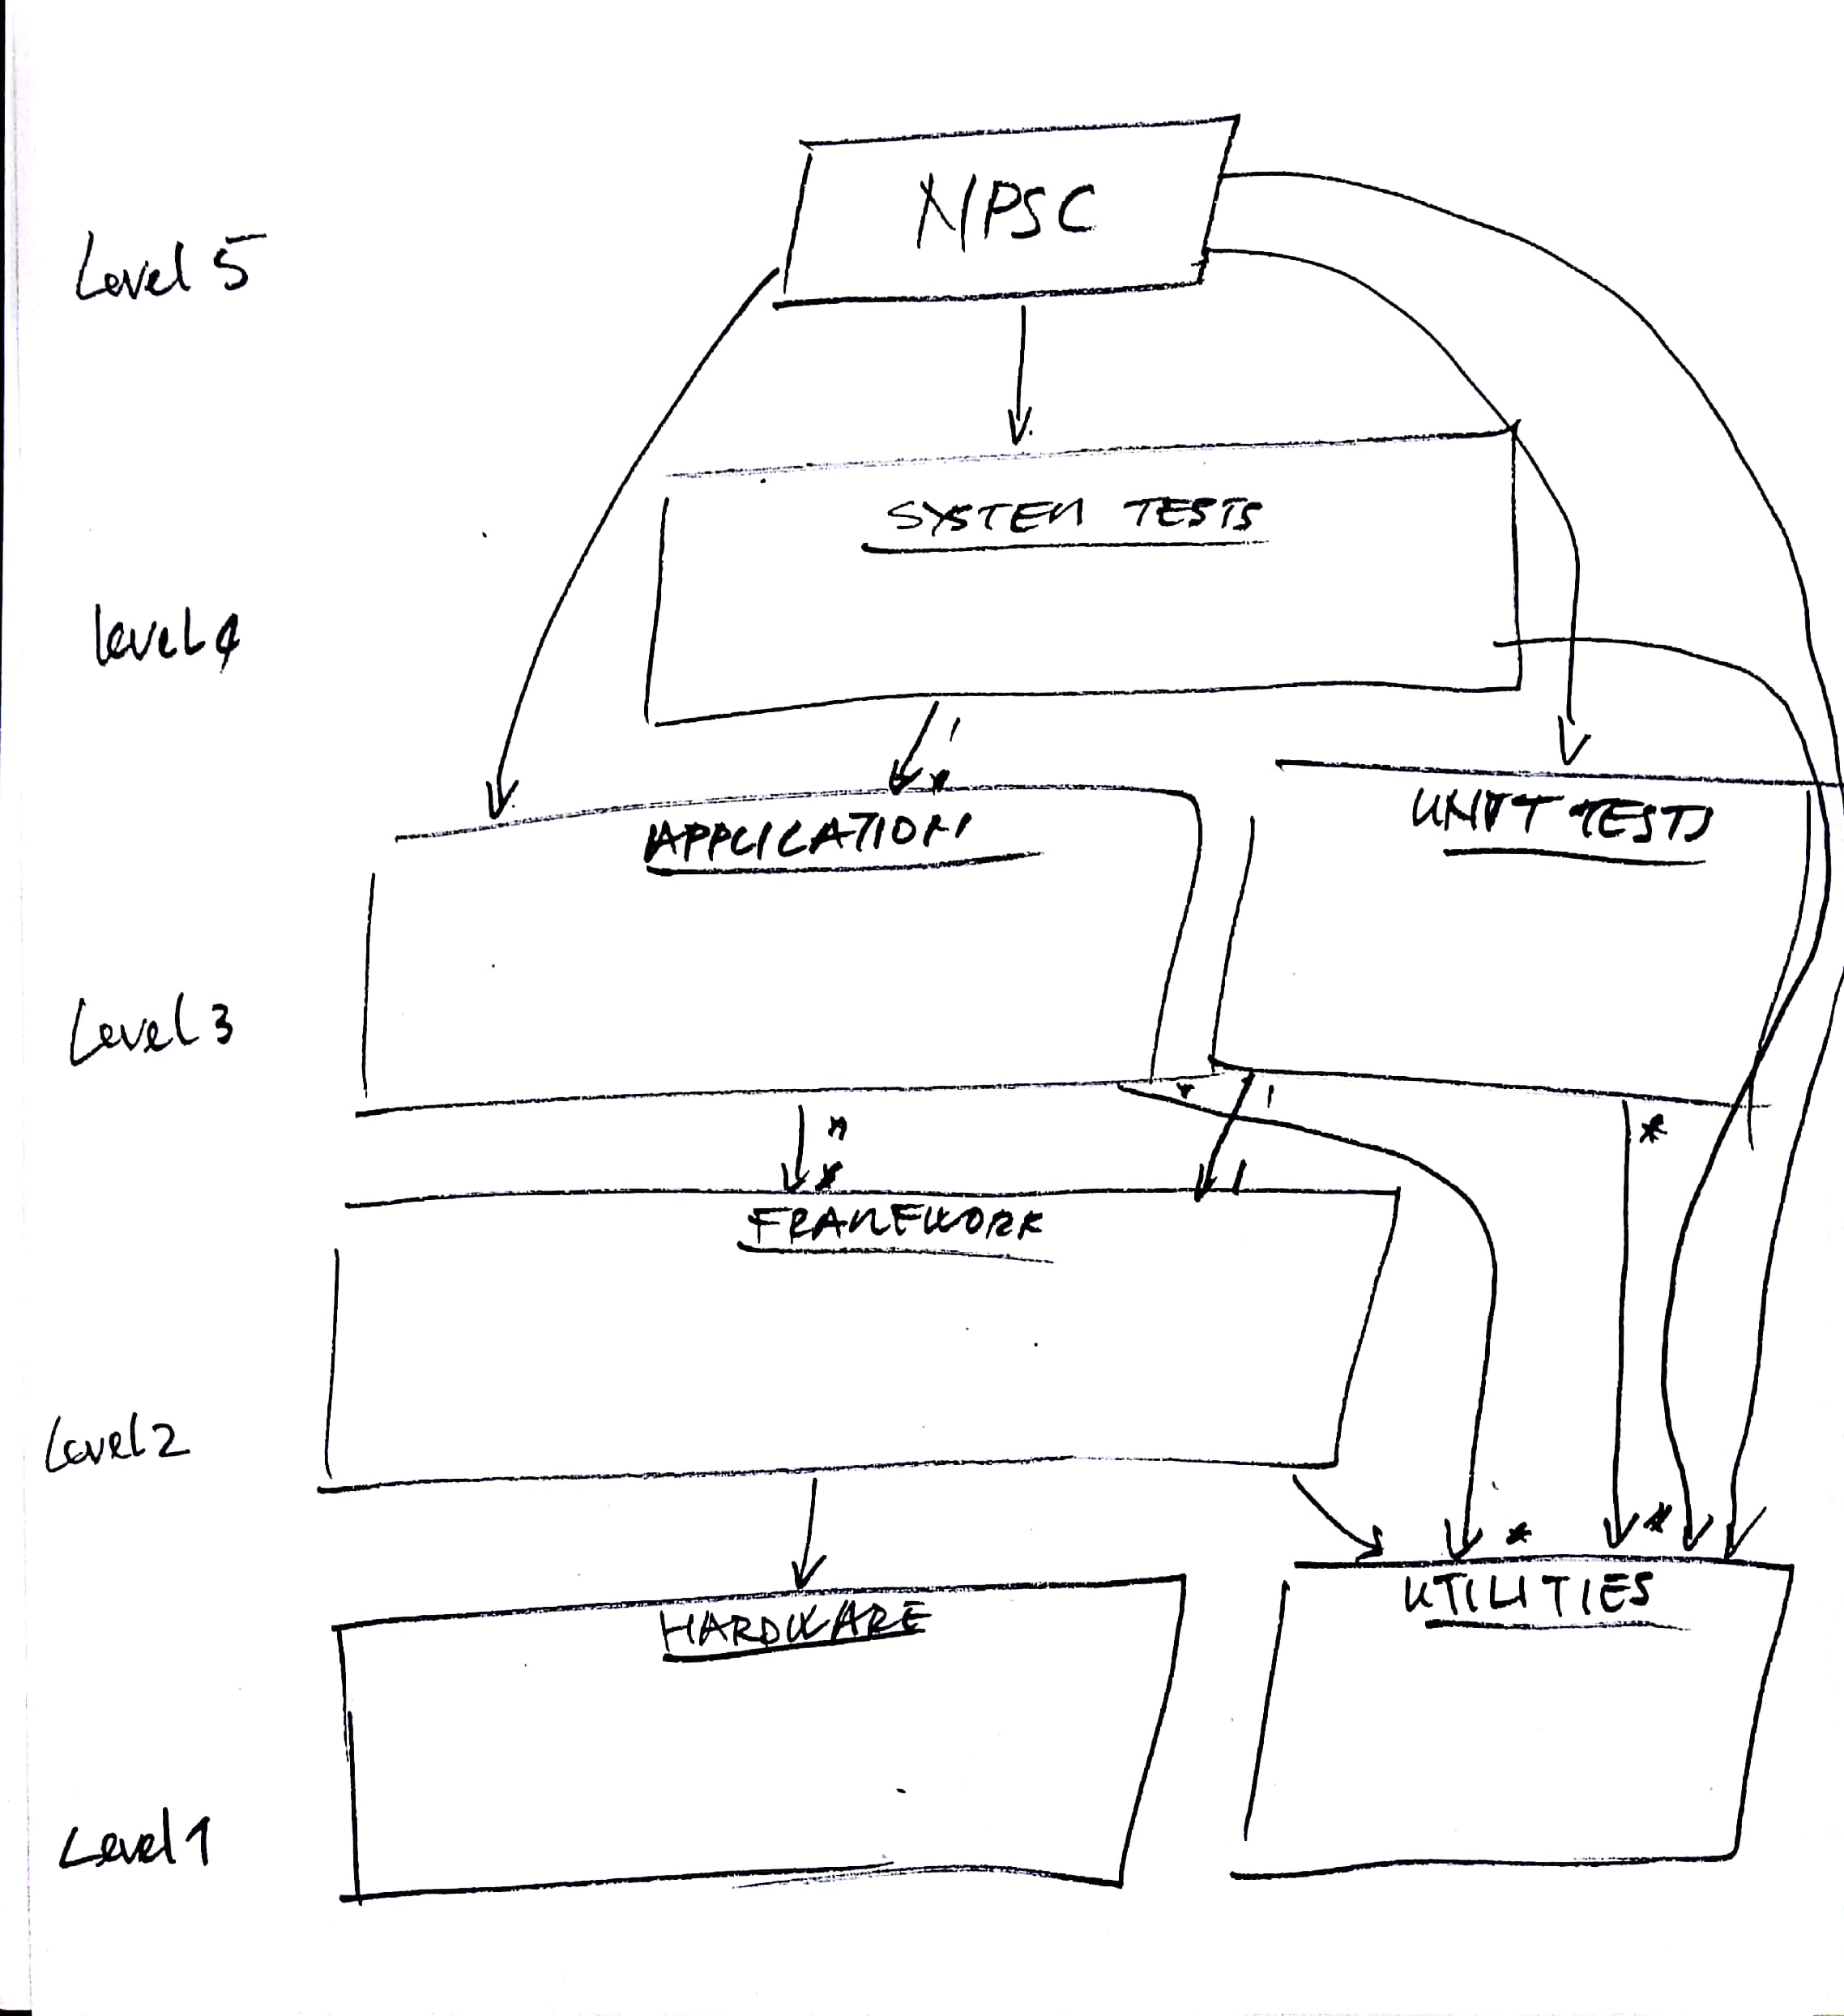
\includegraphics[scale=0.11]{system_overview.jpg}
\caption{Detailed structural block diagram of the NPSC showing the connections between the hardware modules and the main software modules.}
\label{fig:system_overview}
\end{figure}
\begin{itemize}
\item \textbf{Visual application}: This application controls the \textit{Ring}, \textit{Time}, \textit{Weekday}, and \textit{Date} PCBs. It manages visual outputs hardware, from setting the brightness to ensuring that a specific pattern is displayed to ensuring that the desired lux quantity is emitted by the NPSC.
\item \textbf{Alarm application}: This application manages the synchronisation of the internal and external clocks. It is also responsible for managing the alarm stored in the EEPROM and updating the alarm.
\item \textbf{Instruction Queue application}: This application is responsible for the creation of instructions from the user input devices (Nextion touchscreen and Smartphone application) and manages the instruction queue.
\item \textbf{Instruction Fetch Decode and Execute (IFDE) application}: This application relies on the result of the instruction queue application. The IFDE fetches instructions from the instruction queue, decode the instructions and execute commands based on the instruction's opcode. It is the bridge between the user inputs and the hardware modules of the NPSC.
\end{itemize}

%%%%%%%%%%%%%%%%%%%%%%%%%%%%%%%%%%%%%%%%%%%%%%%%%%%%%%%%%%%%%%%%%%%%%%%%%%%%%%%%%%%%
% SECTION: High-level Design
%%%%%%%%%%%%%%%%%%%%%%%%%%%%%%%%%%%%%%%%%%%%%%%%%%%%%%%%%%%%%%%%%%%%%%%%%%%%%%%%%%%%
\section{High-level design}\label{sub_requirements}
This section provides more detailed explanation of the system design requirements broken down into sub-system design requirements. The sub-systems requirements are listed below:
\begin{itemize}
\item Control light pattern
\item Control light parameters
\item Update and obtain time and date from clock
\item Set, edit alarms
\item Store user preferences
\item Control the NPSC using an onboard touchscreen
\item Control the NPSC using a smartphone application
\end{itemize}
The following sections explain the design of the main modules of the NPSC created to meet the system and sub-system requirements.


\subsection{External storage}
The storage's purpose is to store useful information such as the alarm parameters and the user's preferences. Certain applications require storage capability, therefore there is a restricted access to the EEPROM memory. The memory allocation is detailed in \cref{fig:eeprom}.
\begin{figure}[ht]
\centering
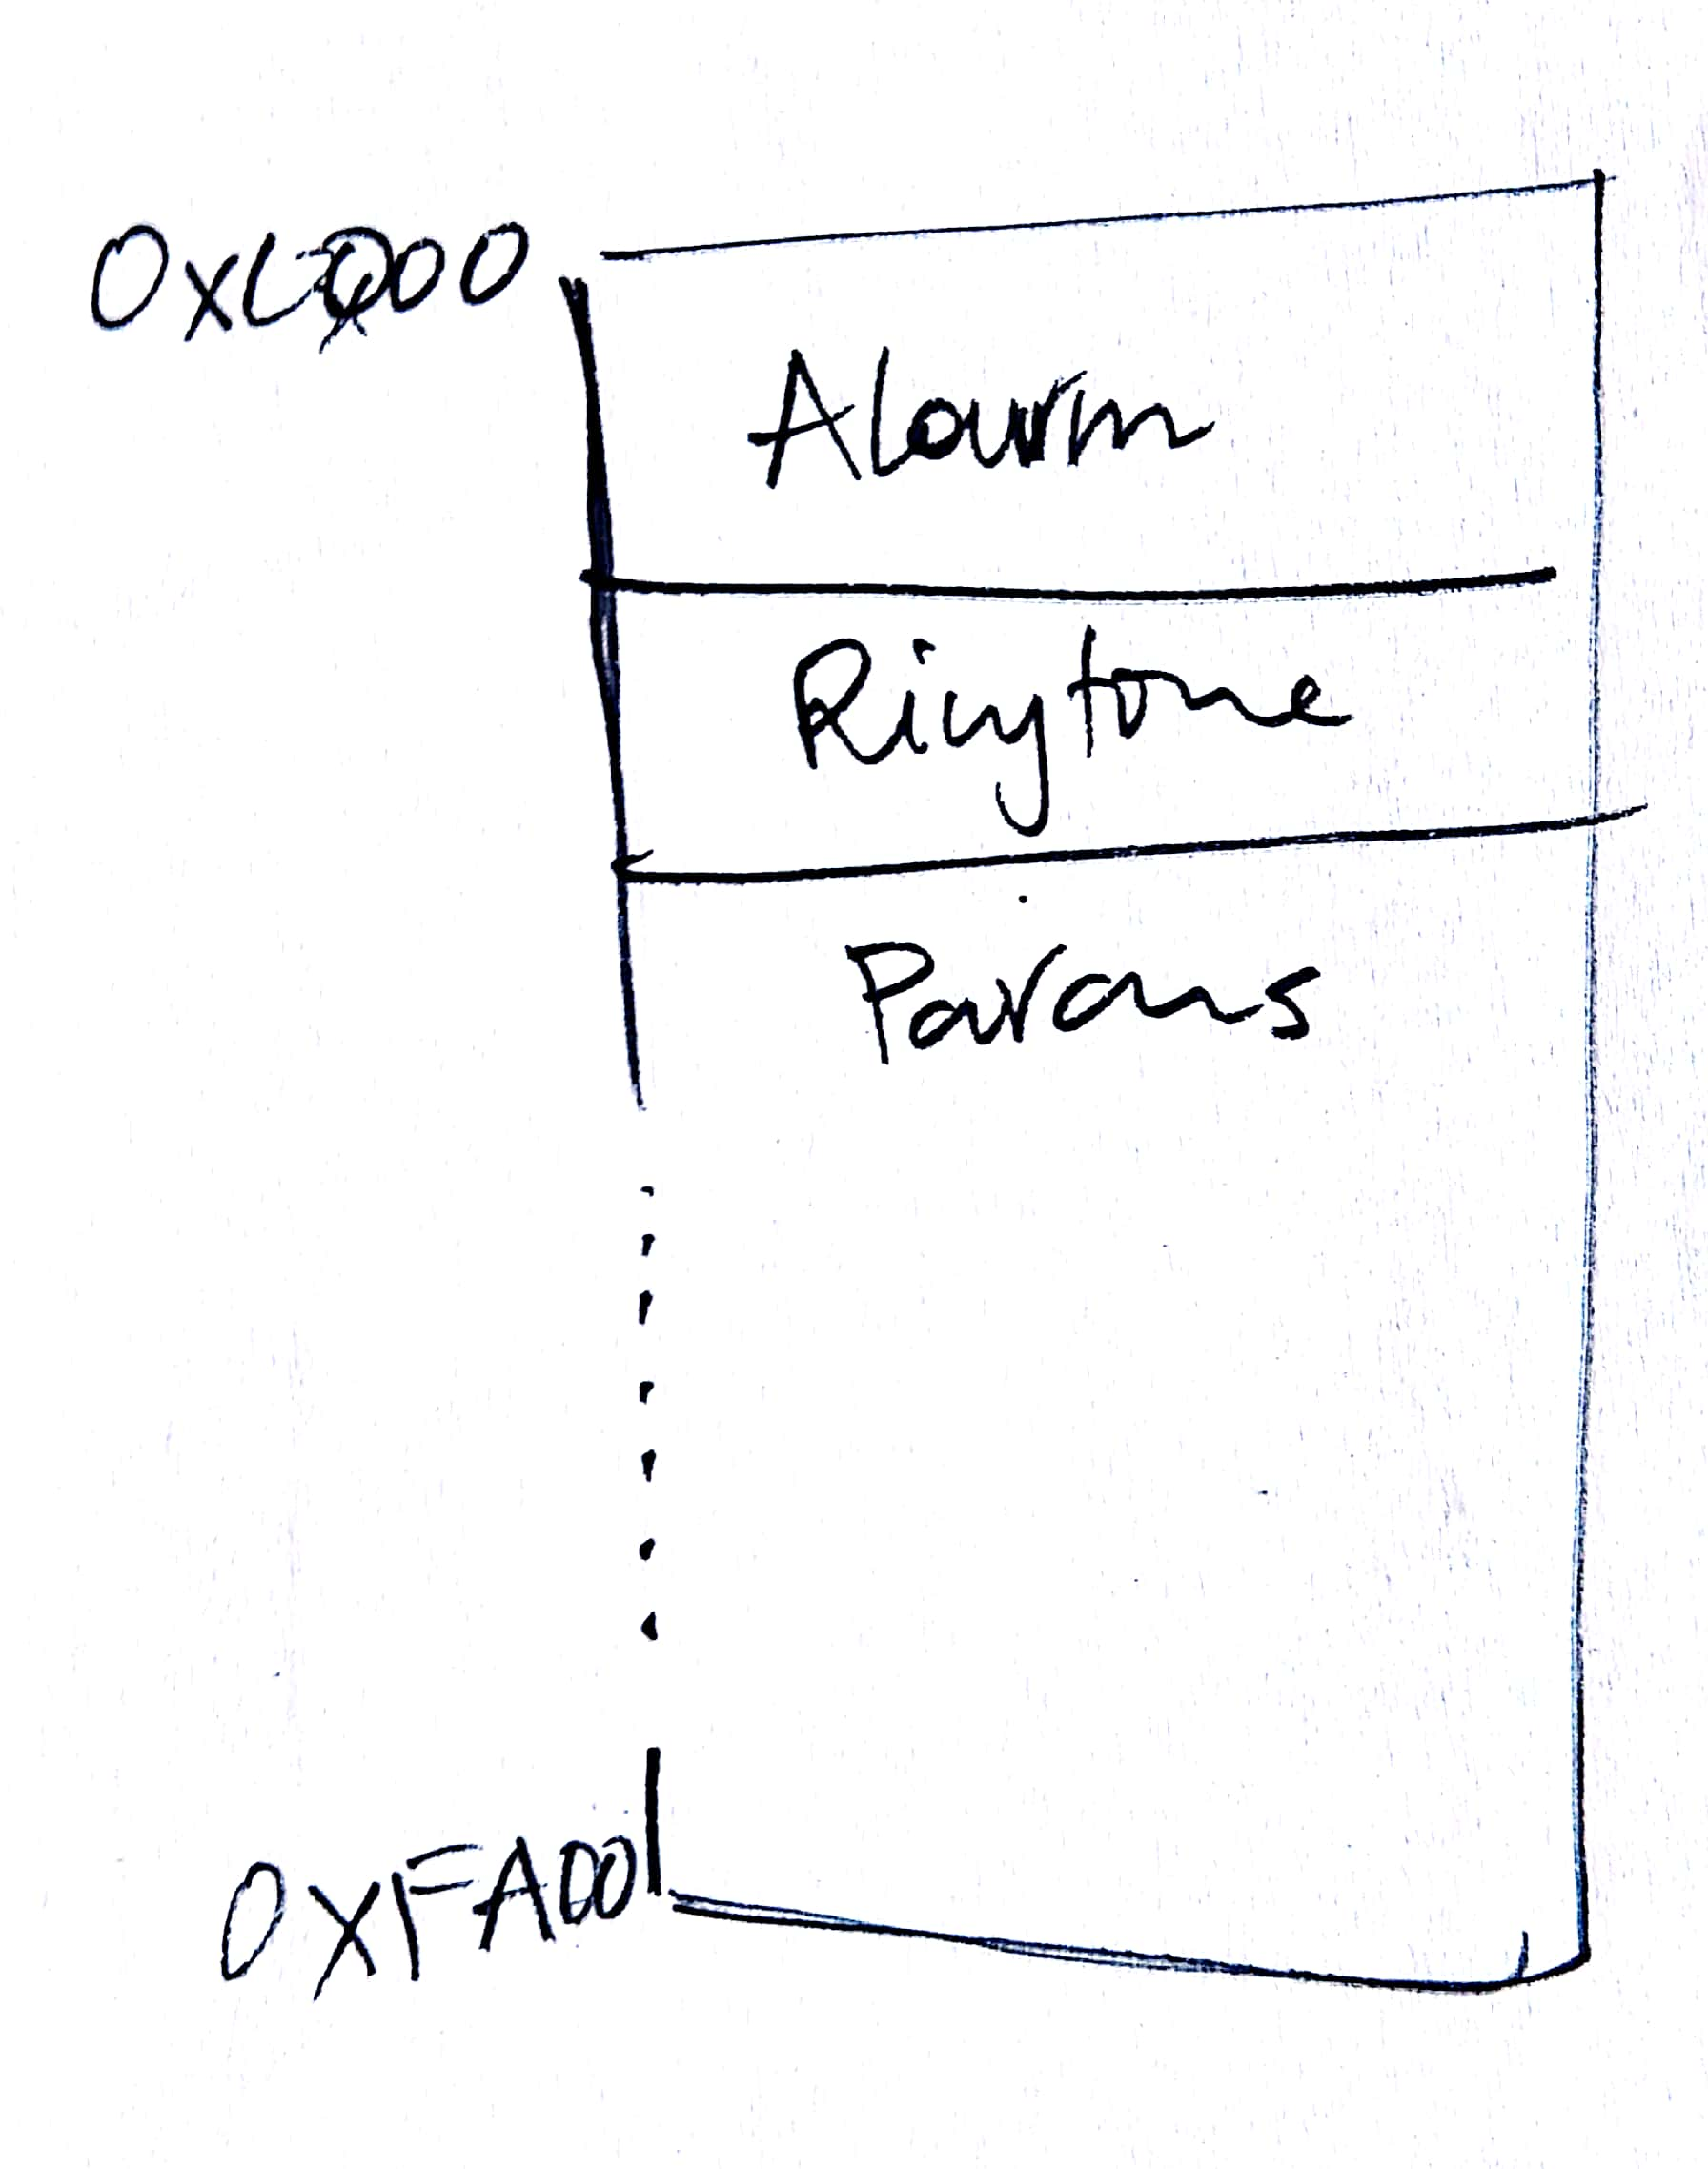
\includegraphics[scale=0.08]{eeprom.jpg}
\caption{EEPROM memory allocation. The first section of the memory is allocated to the alarms, the second to the ringtones and the third section is allocated to the user parameters.}
\label{fig:eeprom}
\end{figure}

\subsection{Inputs/Outputs instruction design}
This section focuses on the design of the user inputs capture and interpretations. \Cref{fig:io_instruction} shows the communication between the microcontroller and the inputs, and the different step through which information sent by these inputs are analysed. 
\begin{figure}[ht]
\centering
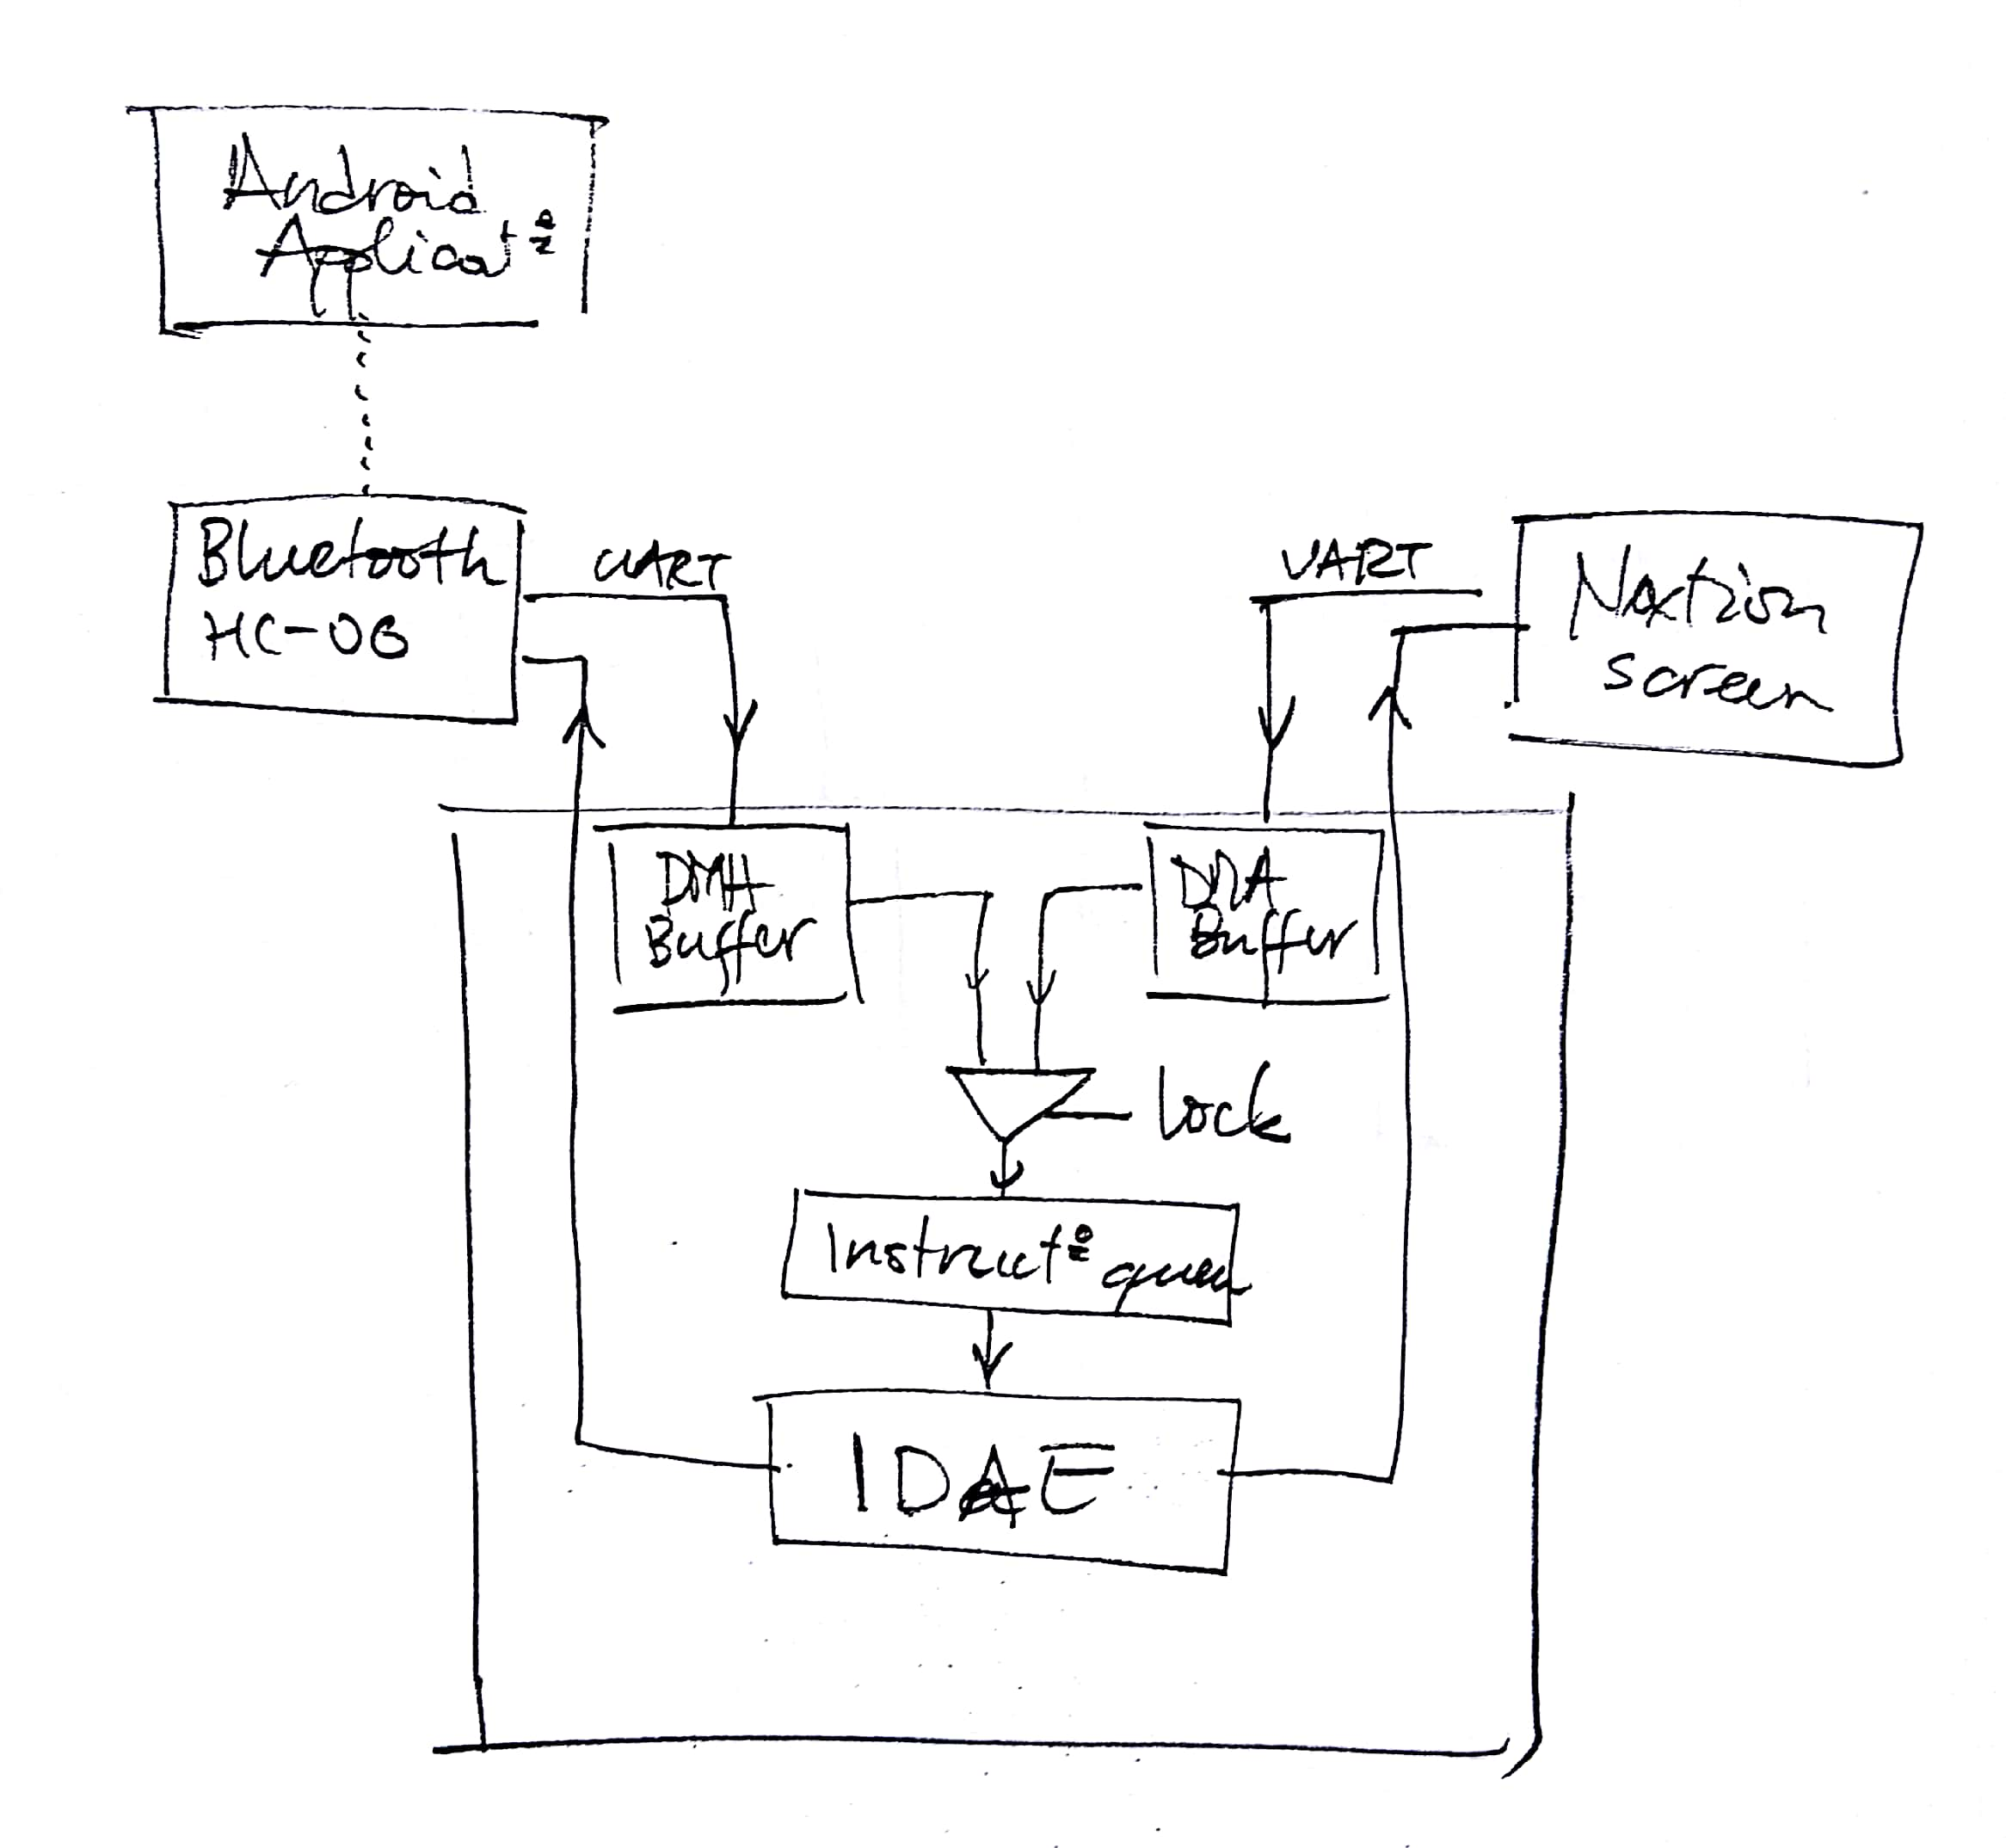
\includegraphics[scale=0.15]{io_instruction.jpg}
\caption{Strutural diagram of the hardware and software modules of the input and output instructions.}
\label{fig:io_instruction}
\end{figure}

\subsubsection{From the inputs to the microcontroller}
There are two user inputs, a smartphone application running on an android device and a nextion screen. The android application communicates with the microcontroller via Bluetooth. Both the Bluetooth device and the Nextion touchscreen use the Universal Asynchronous Receiver-Transmitter (UART) protocol to communicate with the micro. Because the instructions are more than one byte, the microcontroller must be able to receive a stream of bytes with no information loss.\\
To achieve this, each UART uses the Direct Memory Access (DMA) to store each stream received to the corresponding DMA Buffer. After the reception of a stream of data, each DMA Buffer converts its data into instructions which are added to the instruction queue.\\
The DMA function is called on interrupt when the microcontroller receives data on the DMA channel. For this reasons it might occur that one DMA pauses the addition of instruction to the instruction queue by another DMA, and start adding new instructions to the queue. This is a potential concurrency problem that can corrupt the instructions added to the queue. To solve this problem, the addition of instruction to the queue is considered as a critical section of the design. A lock is thus added to the instruction queue such that only a process owning the lock can add new instructions to the queue.\\
The instruction queue is a First In First Out (FIFO) queue, meaning that an element removed from the queue was the oldest element in the queue. This allows the instruction to be executed in order of arrival.

\subsubsection{Instruction Fetch Decode Execute (IFDE)}
The IFDE act as the Central Processing Unit (CPU) of the NPSC. Its role is to fetch instructions from the instruction queue, decode the instructions and execute them by calling the corresponding methods. It is the brain of the NPSC operation and acts as a bridge between the user inputs and the different hardware module. As the IFDE uses specific instruction set, there is a restriction on the actions performed by the users reducing any security breaches. By using an instruction set and the IFDE, the functionalities of the NPSC can easily be expanded and modify during the software development.
 
\subsubsection{Buffer size and Instruction sets}
The instruction size was mostly defined by the rules of the Nextion touchscreen. This touchscreen is able to send information to a microcontroller using UART. However, it does not send a single byte of data unless a character is sent. As it is not convenient to convert all the integer parameters into characters, the second build-in method used by the nextion to send information was considered. This method sends an integer value as four bytes of data. Because certain methods of the framework require structs \footnote{A struct also known as a record is a collection of data type used to represent entities having multiple attributes} as parameters, the instruction size was set to be double the size of the number of bytes sent by the nextion touchscreen per each method call. \\
The DMA Buffer size is dependent on the design of the Nextion touchscreen application and the Android application, as a stream of instruction might be sent. The number of instructions in the queue is also dependent on the DMA Buffer size because there are two inputs and therefore two DMAs, a rule of thumb for the instruction queue size is to be at least the number of inputs multiply by the DMA Buffer size.\\

The instructions of the NPSC are listed in \cref{table:instruction_set}. The instructions are divided into categories, each category represent the actions performed at a framework level or application level (see \cref{fig:system_hierarchy}). There are two types of instructions, the set instructions and the get instructions. The set instructions write informations to the NPSC while the get information are just signal indicating that the user input device is requesting information. The instrcutions are 8 bytes long and the first byte represent the opcode of the instrucion while other byte are for the data sent. Instructions of the same category have the same most significant four bytes, for example all intructions from the Alarm category have $0x1*$ as their opcode with $*$ being any one digit hexadecimal number. The pcode 0x00 is reserved for identifying data that must not be converted into instructions.
\begin{landscape}
\begin{table}[t!]
\centering
\caption{Instruction set used for the control of the NPSC by the users. Each instruction has a category, a name and an opcode. \textbf{-} in the table indicates data that will not be used by the IFDE. \textbf{*} indicates character data.}
\label{table:instruction_set}
\begin{tabular}{cccccccccc}
\hline
\hline
\multicolumn{10}{c}{Instructions} \\
\toprule
\multirow{2}{*}{Category} & \multirow{2}{*}{Name} & \multicolumn{8}{c}{Instruction bytes} \\
& & \textbf{M0/opcode} & \textbf{M1} & \textbf{M2} & \textbf{M3} & \textbf{M4} & \textbf{M5} & \textbf{M6} & \textbf{M7} \\
\hline
\toprule
\multirow{2}{*}{External RTC} & set clock & \textbf{0x01} & year & month & date & weekday & hour & minute & second \\
& get clock & \textbf{0x02} & - & - & - & - & - & - & - \\
\midrule
\multirow{6}{*}{Alarm} & set alarm time parameters & \textbf{0x10} & id & hour & minute & date/day selection & day/date & repeat & - \\
& set alarm extra parameters & \textbf{0x11} & id & ringtone & pattern & enable & fetch & - & - \\
& set alarm label & \textbf{0x12} & id & label number & - & * & * & * & * \\
& set alarm enable & \textbf{0x13} & id & enable & - & - & - & - & - \\
& get alarm minimum parameters & \textbf{0x14} & id & id & - & - & - & - & - \\
& get alarm parameters & \textbf{0x15} & id & - & - & - & - & - & - \\
\bottomrule
\hline
\end{tabular}
\end{table}
\end{landscape}

\subsection{Input devices}
HOW ARE THE USER APPLICATIONS DESIGNED?

\subsection{Alarm and Clock}
The structural diagram of this module is shown in \cref{fig:alarm_clock}. The microcontroller used by the NPSC has a built-in RTC with two alarms (alarm A and alarm B), this module makes use of an Alarm manager (application software) which control the EEPROM, the external and internal RTCs and the two alarms.
\begin{figure}[ht]
\centering
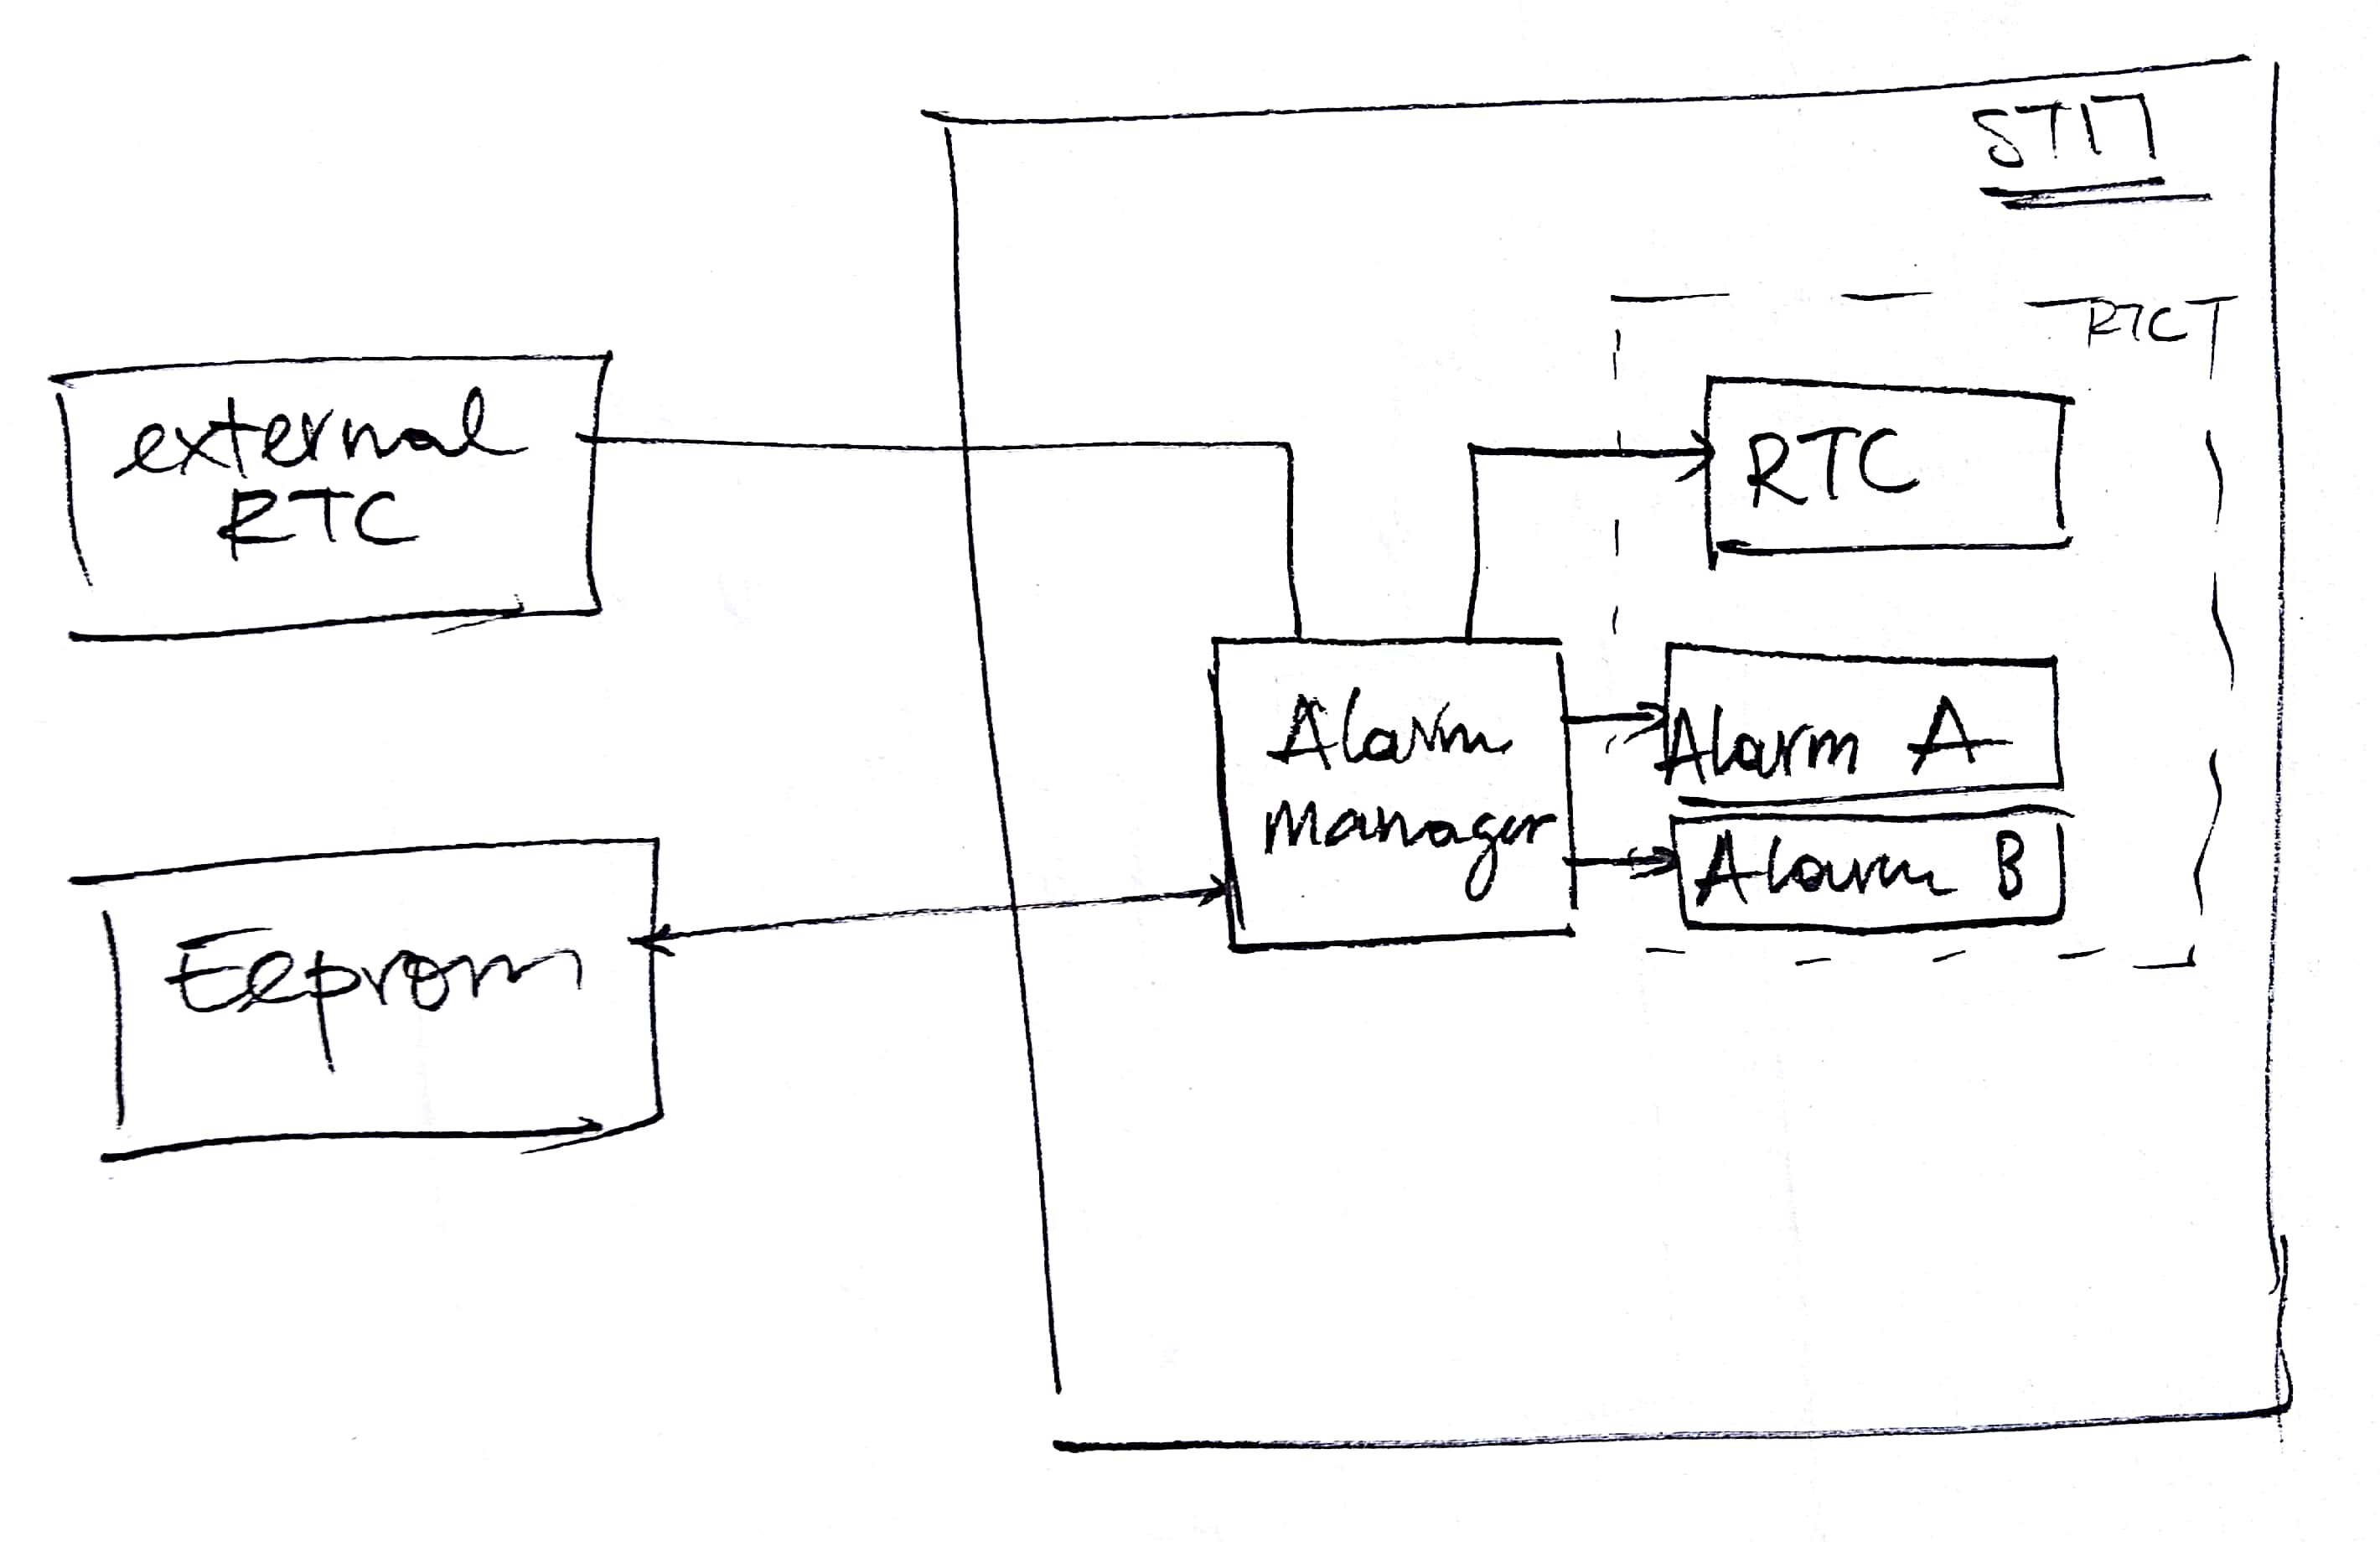
\includegraphics[scale=0.11]{alarm_clock.jpg}
\caption{Structural diagram of the hardware and software module used in the alarm-clock application.}
\label{fig:alarm_clock}
\end{figure}
Alarm A and B are triggered based on the comparison of their time with the internal RTC of the STM. As for the internal (built-in) RTC, it relies on the crystal oscillator of the STM to update its time. This RTC is power dependent and loses its time when the STM is powered off. To prevent manual update of the time everytime the STM is powered on, an external clock module must be used. For this prototype, the DS1307 RTC is used as the external clock module. This RTC is not very accurate, in many applications, it has lost few minutes of accuracy every day. This prototype is a proof of concept and is focused on the light requirements and not the accuracy of the clock, therefore, the DS1307 will be used. Later versions of the NPSC could use more accuracy clock module such as a GPS or more accurate RTC.  \\
On power on, the Alarm manager synchronises the internal clock with the external clock by loading the external RTC's time and date to the internal RTC. It then loads two alarms from the EEPROM which are supposed to be triggered before the others and set these alarms to alarm A and alarm B from the internal RTC. The Alarm manager is also responsible for storing the alarms to the EEPROM and updating then when an alarm goes off. 

\subsection{Visual outputs}
The visual outputs are all modules related to the control and emission of light in the system. \Cref{fig:visual_outputs} illustrates the interaction between these modules and the STM. 
\begin{figure}[ht]
\centering
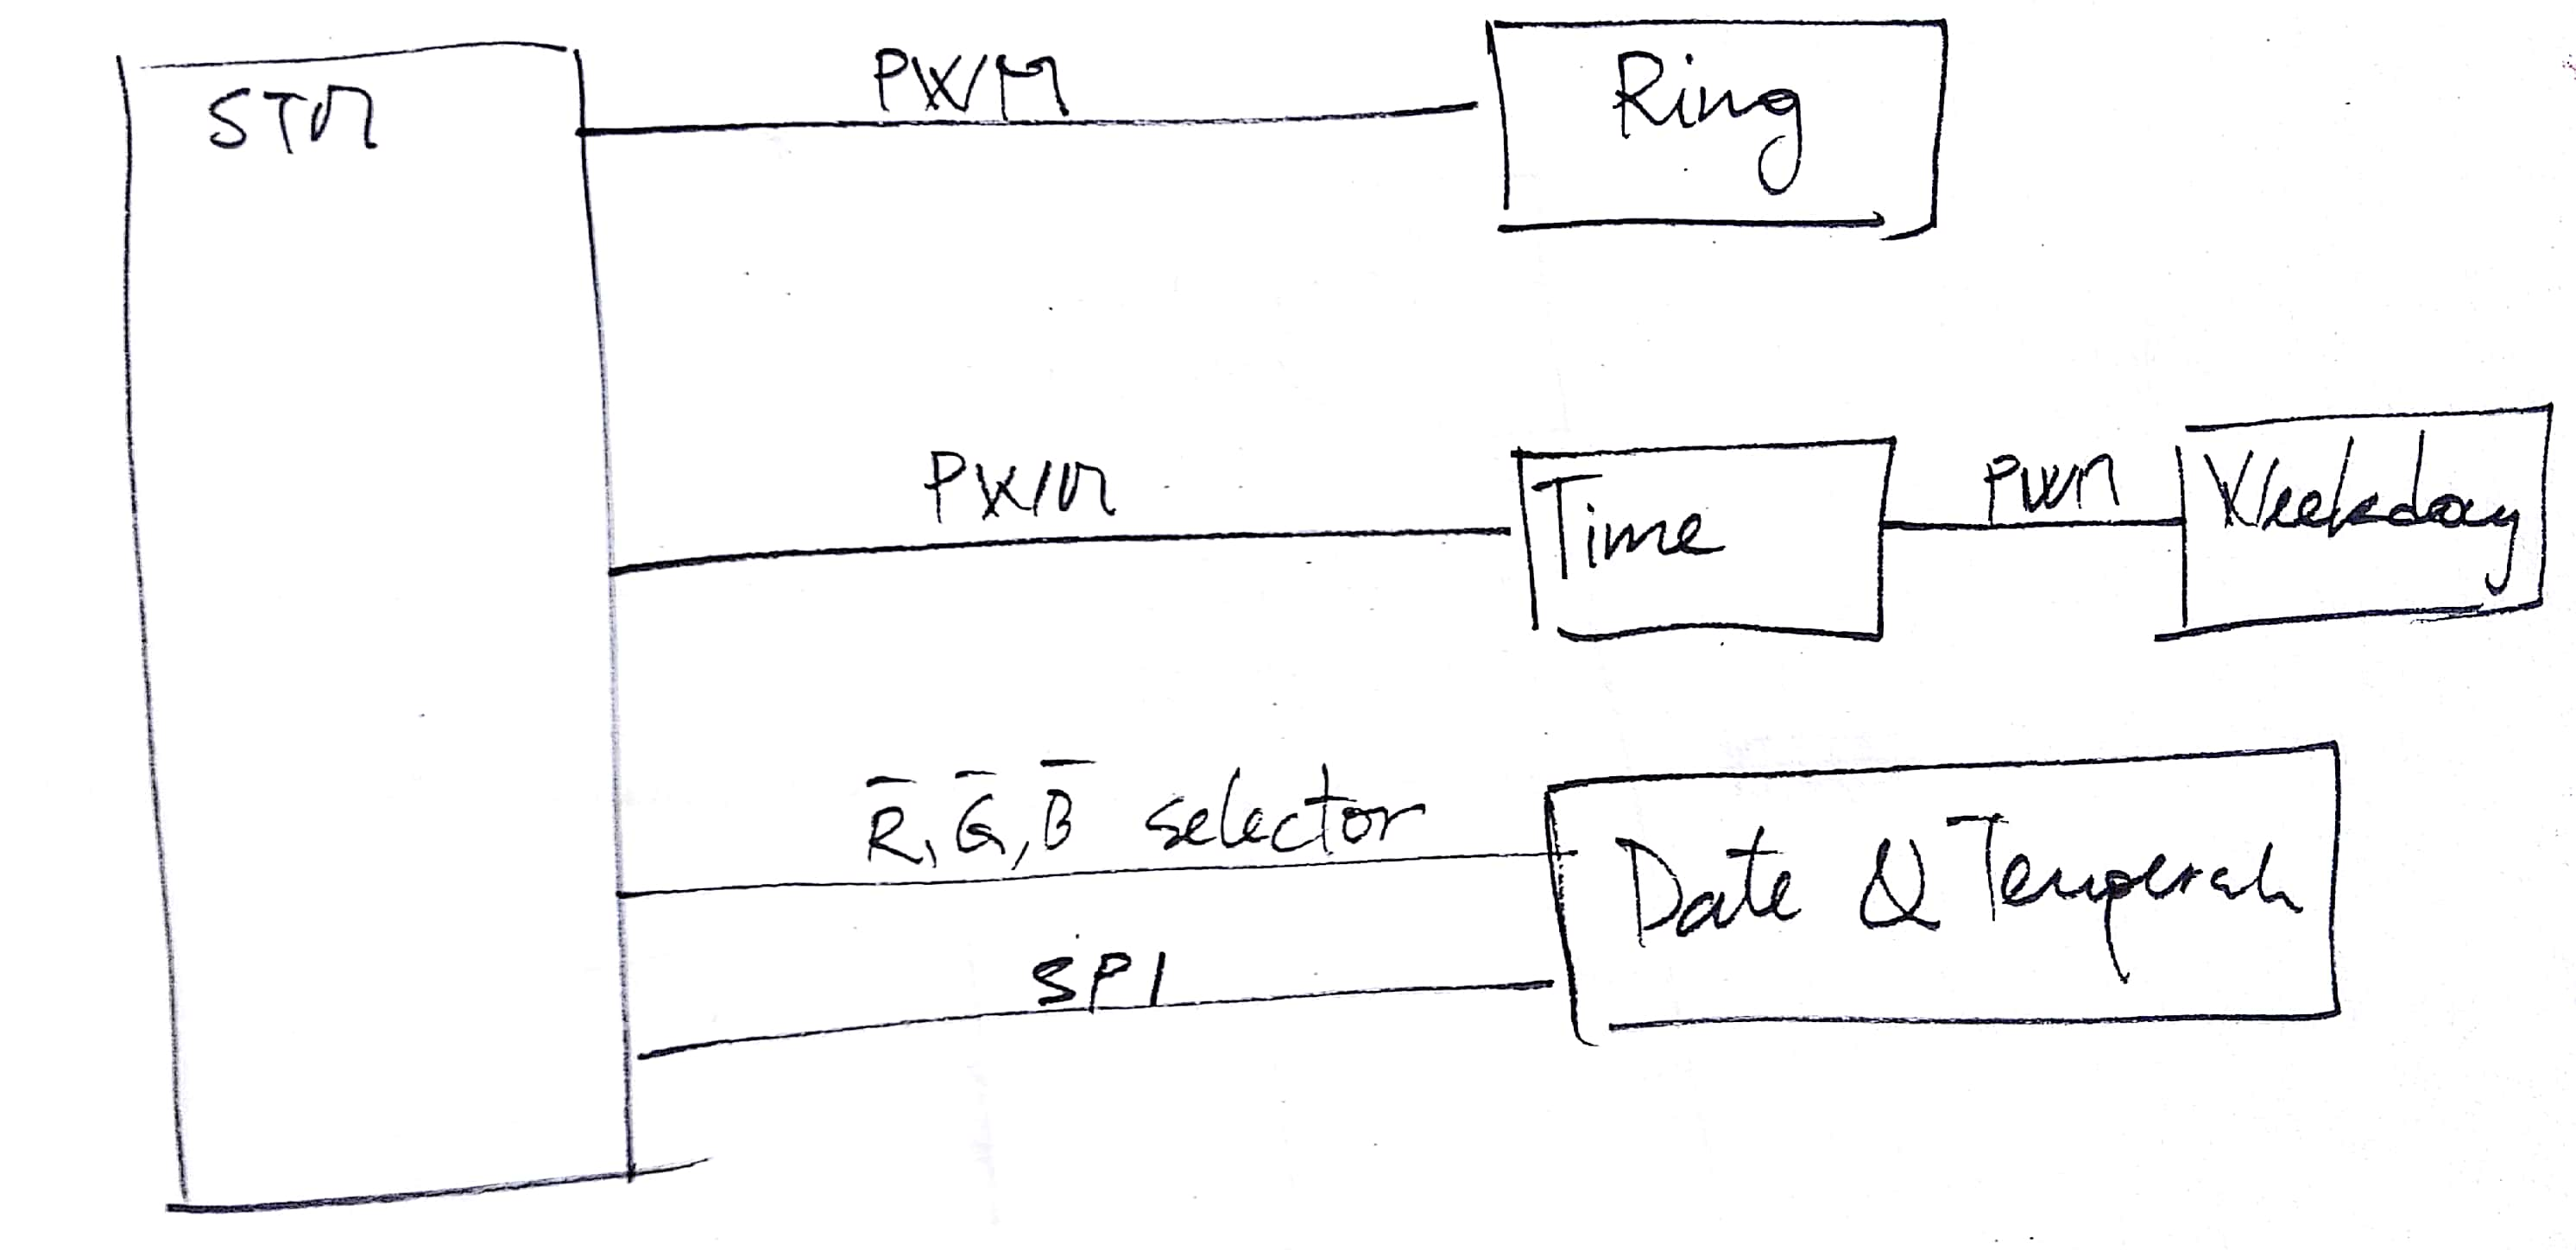
\includegraphics[scale=0.12]{visual_outputs.jpg}
\caption{Structural diagram of the hardware and software used for the visual outputs.}
\label{fig:visual_outputs}
\end{figure}
There are two types of hardware modules, the first type (type 1) of modules is a series of neopixels connected in cascade controlled by Pulse Width Modulation (PWM), the second type (type 2) of modules are controlled using a Serial Peripheral Interface (SPI) bus. All type 1 modules inherit the ability to be connected in cascade from the neopixels; however, the ring is the only light source used to affect the human sleep-wake cycle, it is essential that its control is separated from another type 1 module. The two other type 1 is designed to display time and date information, therefore, they can be combined as one module. The only type 2 module in the visual outputs is the Date PCB, this PCB is designed to display the date, the month and the room temperature.\\
For consistency in the visual, RGB 7 segments displays are used for the Date PCB. Moreover, the Time PCB uses neopixels as no RGB 7 segments displays bigger than the ones used for the Date PCB could be found.\\
The visual outputs are controlled by the Visual manager from the visual application. The Visual manager's role is to update the neopixel buffer for each type 1 module according to the visual parameters set by the user. These parameters consist of RGB colours, the brightness, the location of the pixel \footnote{The location is the number of the neopixel of interest in the series of neopixel on a specific module. On the Ring PCB, location 61 is the first neopixel on the second ring.}. At a higher level of control, these parameters also include module's pattern, mode and duration. The Visual manager is also responsible for updating information on the Date PCB.   

\subsection{Sensors}
There are two sensors on the NPSC, a temperature sensor and a photoresistor. The role of the temperature sensor is to get the room temperature. The photoresistor has a more interesting purpose; it is used to obtain the light intensity outside the NPSC in order to allow the system to adjust the neopixel brightness such that the required illuminance does not vary by a significant margin at the user's location.



%%%%%%%%%%%%%%%%%%%%%%%%%%%%%%%%%%%%%%%%%%%%%%%%%%%%%%%%%%%%%%%%%%%%%%%%%%%%%%%%%%%%
% SECTION: Detailed design
%%%%%%%%%%%%%%%%%%%%%%%%%%%%%%%%%%%%%%%%%%%%%%%%%%%%%%%%%%%%%%%%%%%%%%%%%%%%%%%%%%%%
\section{Details hardware design} \label{design}
This section provides detailed information on the design of the hardware modules. Off the shelves, hardware modules are not detailed in this sections as these modules already have the necessary information on their datasheets. All datasheets are in \ref{datasheets} and in the repository on GitHub. 

\subsection{Neopixels boards}
The type 1 modules are made up of series neopixels connected in a daisy chain fashion. Each neopixel has two power pins and two data pins as illustrated by \cref{fig:neopixel_sch}. The stream of bytes is received by the neopixel at its DIN pin, after extracting the first 24 bytes, the neopixel transmit the truncated stream to the DOUT pin. By connecting the DOUT pin of one neopixel to the DIN pin of the next neopixel, a single stream of bytes can be used to program all neopixels in the series. 
\begin{figure}[ht]
\centering
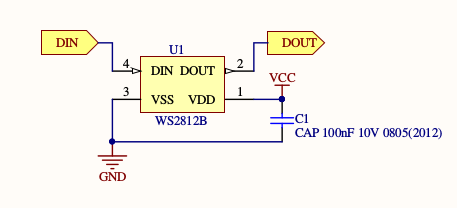
\includegraphics[scale=0.5]{neopixel_sch.png}
\caption{Schematics of one neopixels receiving data from DIN and transmitting data to DOUT.}
\label{fig:neopixel_sch}
\end{figure}
Although all type 1 module uses the sample principle, each module has more specific features in its design.
\subsubsection{Ring PCB}\label{ring_pcb}
This module has 180 neopixels physical positioned such that they form three rings of 60 neopixels each. Unlike the neopixel in \cref{fig:neopixel_sch}, there is one capacitor per five neopixels. The daisy chain is broken at every $15^{th}$ neopixels for debugging the data stream. \\
As mentioned in \cref{table:neopixel_specs}, each neopixel requires $20mA$ per colour. The ring uses 180 neopixels thus a current of $20*3*180 = 10800 mA$ is expected to be drawn by the Ring. Following the IPC2221 standard, the board width was calculated with a current of $12A$ (worst case scenario), a board thickness of $1oz/ft^2$ and a temperature rise of $15^oC$; the required trace width of the external layers must be at least \textbf{9.84mm}. This is a stringent requirement on the NPSC as the ring must be contained in a $25*25*10cm^3$ case. With an expected an inner radius of $6.5cm$ and an outer radius of $10.5cm$, the Ring has approximately a surface area of $ \pi*(10.5^2-6.5^2) = 213.63 cm^2$ on each side for dissipating its heat. Furthermore, the neopixel pins have a pad on $0.6*1.5 mm^2$ while the width of the power line must be at least $9.84mm$. Each ring has 60 neopixels thus $60*9.84=$ \textbf{590.4mm} is required as the width of the power line per ring. However, the minimum circumference of the ring is $65*2*\pi$ = \textbf{408.41mm} which is less than what is required. With this conditions, the board is expected to have a higher temperature rise.\\
The schematic and PCB of this board are shown in \cref{fig:ring_sch_pcb}.

\subsubsection{Time}
This board has its series of neopixels physically placed on the board such that they simulate four RGB seven segment display. The board is made generic so that each display can be controlled by its own data pin. The board also has the ability to be controlled all display using the first display controller pin, this is done by connecting the DOUT of the last neopixel of a display to the DIN of the first neopixel in the next display.
The schematic and PCB of this board are shown in \cref{fig:time_sch_pcb}.

\subsubsection{Weekday}
This board has only seven neopixels in its series, one for each day in the week. It gets its input (DIN) from the output (DOUT) of the Time PCB.
The schematic and PCB of this board are shown in \cref{fig:weekday_sch_pcb}.

\subsection{Date and Temperature PCB}
This PCB uses six seven segments display to display the date, the month and the room temperature. \Cref{fig:date} shows the simplified schematic of this module. The seven segment used is the ACD8143 which contain a pair of RGB seven segments display. In order to reduce the number of pins used to control these displays, the serial interfaced 8-digits LED driver display (MAX7219) was used. It uses SPI to control the segments of all the displays. It controls the displays by continuously selecting each display in a loop and setting the segments to the desired voltage. The MAX7219 is not designed for RGB seven segments displays, therefore, additional circuits composed of R, G, B signals and NOT gates were used such that on display selection, the display has the colour set by the R, G, B selectors.   
\begin{figure}[ht]
\centering
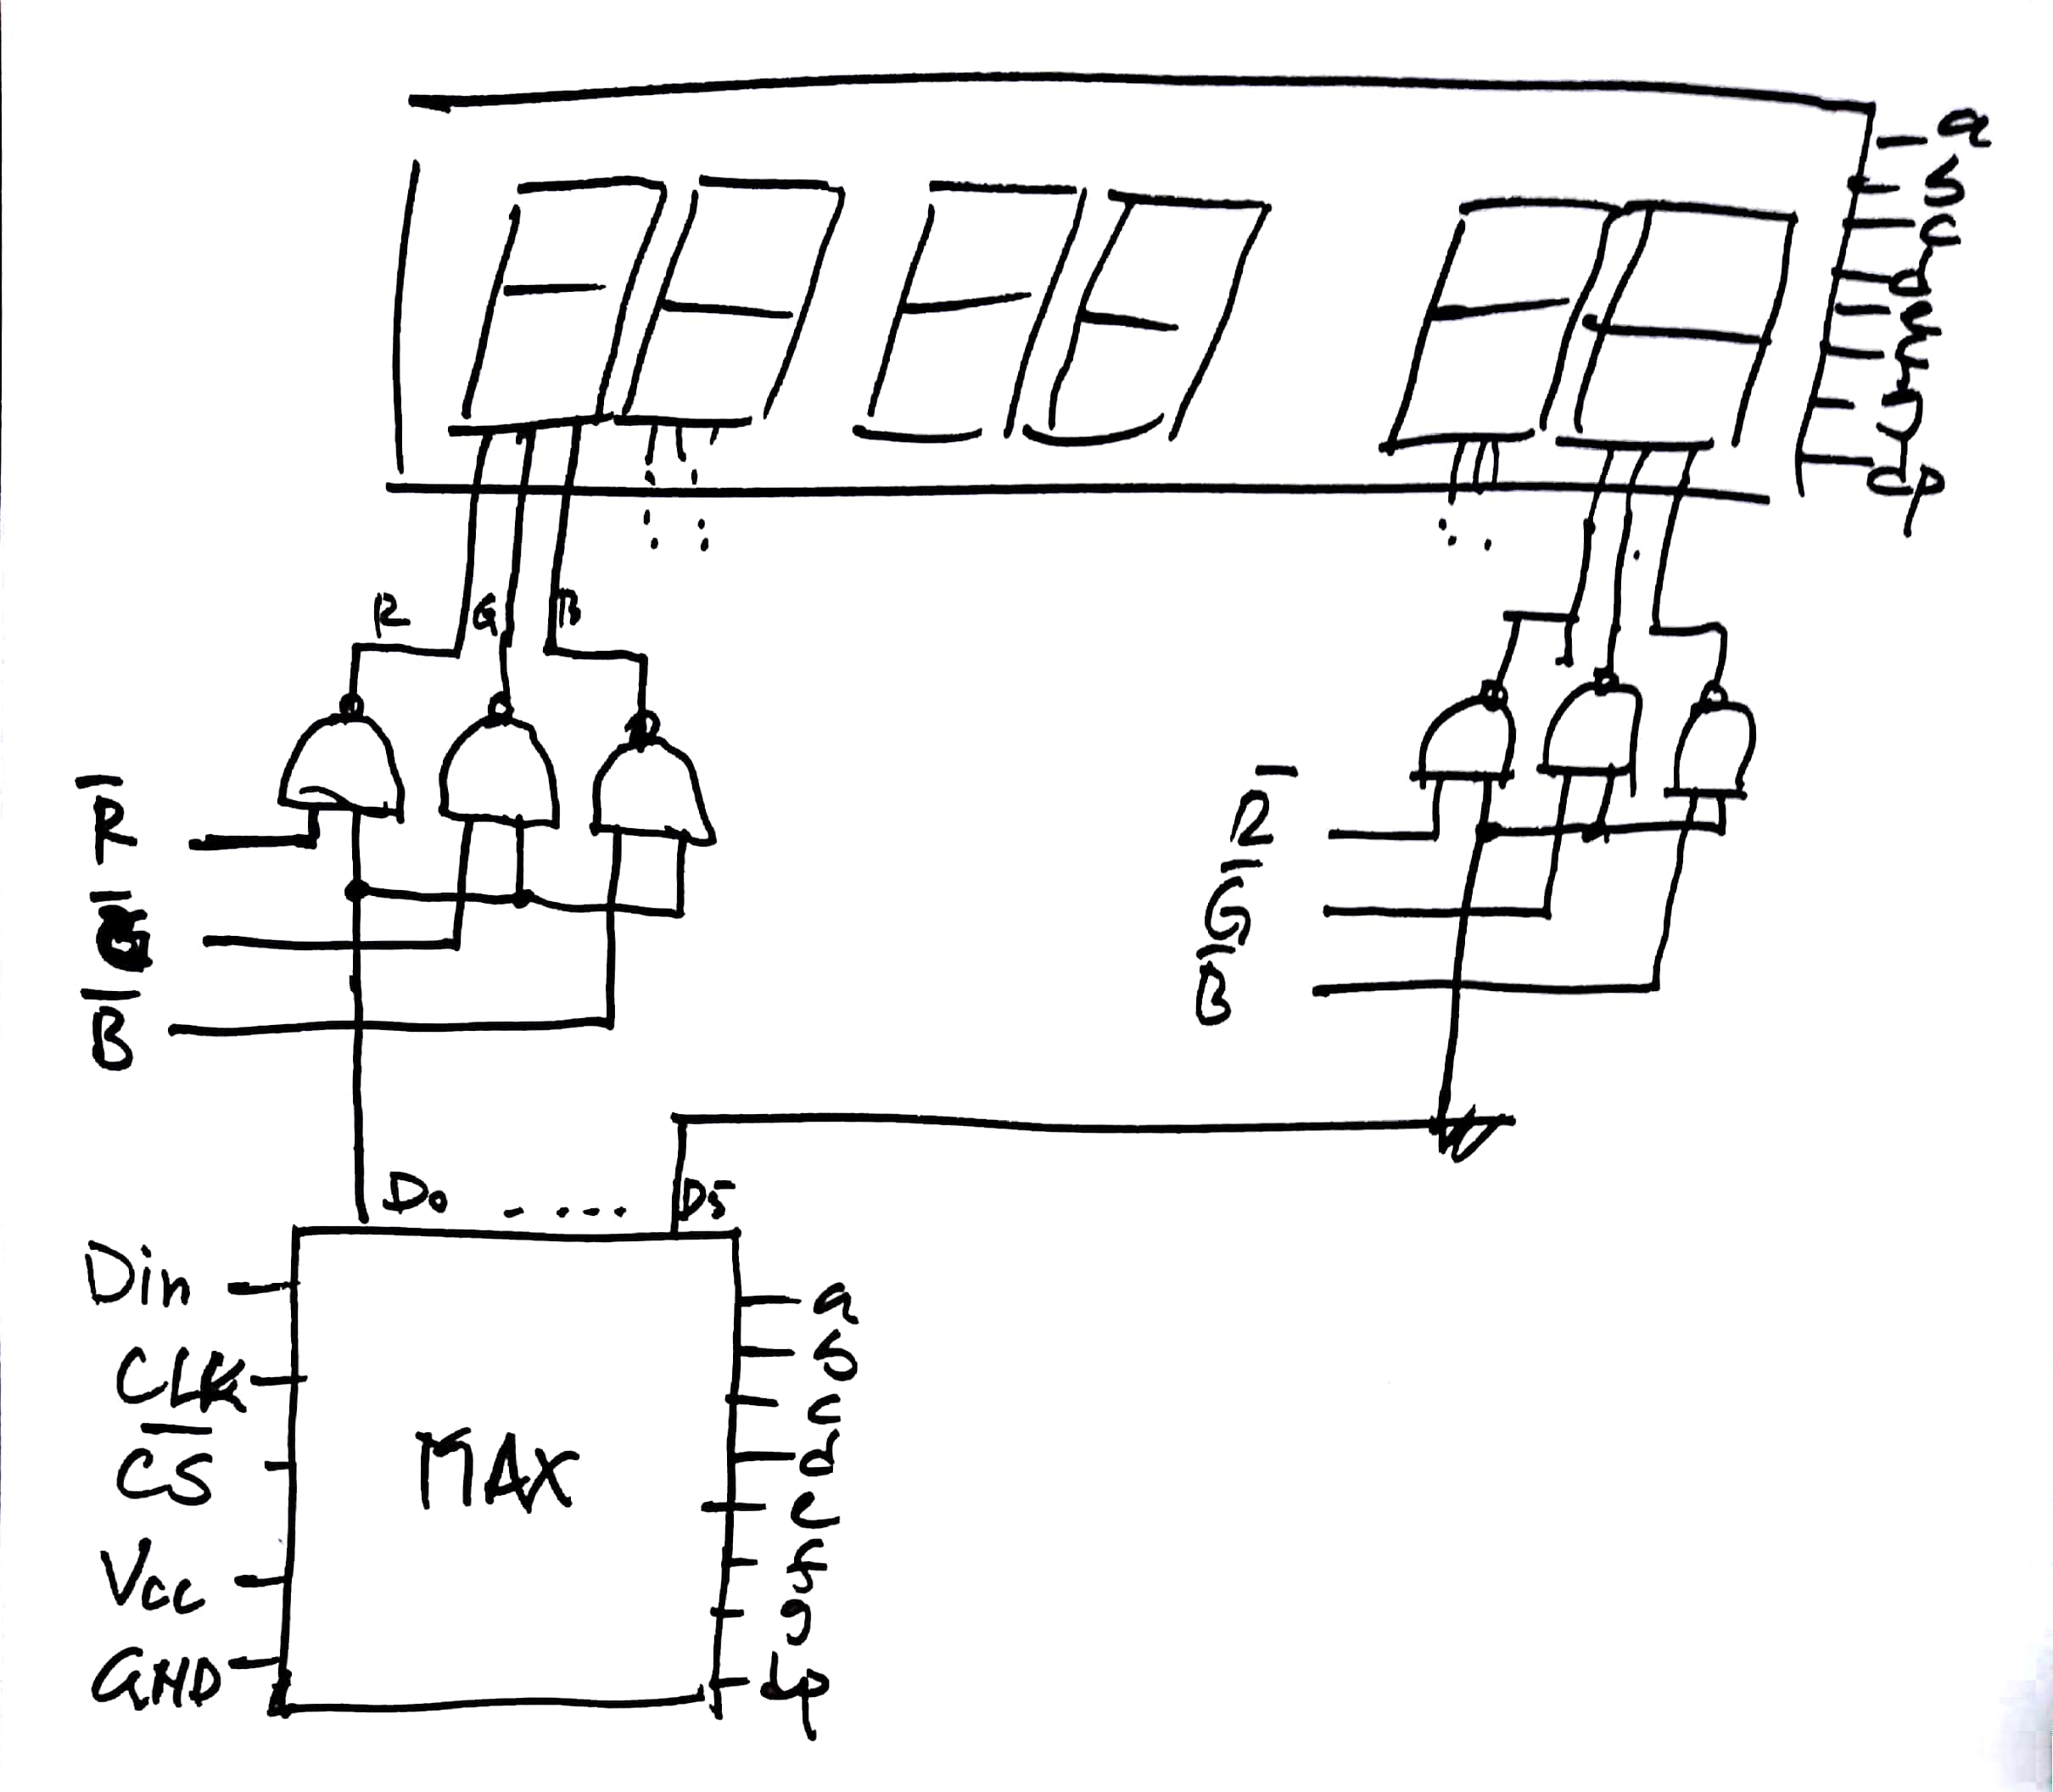
\includegraphics[scale=0.1]{date.jpg}
\caption{Simplified schematic of the Date and Temperature circuit.}
\label{fig:date}
\end{figure}
\chapter{Implementation}
This section provides information on the software implementation of the NPSC. Refering to the system hierarchy illustrated in \cref{fig:system_hierarchy}; this section focuses on the utilities at level 1, the framework at level 2, the applications at level 3 and the main at level 5.
   
%%%%%%%%%%%%%%%%%%%%%%%%%%%%%%%%%%%%%%%%%%%%%%%%%%%%%%%%%%%%%%%%%%%%%%%%%%%%%%%%%%%%
% SECTION: Utilities
%%%%%%%%%%%%%%%%%%%%%%%%%%%%%%%%%%%%%%%%%%%%%%%%%%%%%%%%%%%%%%%%%%%%%%%%%%%%%%%%%%%%
\section{Utilities}
Each module to have table describing each methods used\\

%%%%%%%%%%%%%%%%%%%%%%%%%%%%%%%%%%%%%%%%%%%%%%%%%%%%%%%%%%%%%%%%%%%%%%%%%%%%%%%%%%%%
% SECTION: Framework
%%%%%%%%%%%%%%%%%%%%%%%%%%%%%%%%%%%%%%%%%%%%%%%%%%%%%%%%%%%%%%%%%%%%%%%%%%%%%%%%%%%%
\section{Framework}
Subsection for each module.\\
Each module to have table describing each methods used\\

%%%%%%%%%%%%%%%%%%%%%%%%%%%%%%%%%%%%%%%%%%%%%%%%%%%%%%%%%%%%%%%%%%%%%%%%%%%%%%%%%%%%
% SECTION: Applpication
%%%%%%%%%%%%%%%%%%%%%%%%%%%%%%%%%%%%%%%%%%%%%%%%%%%%%%%%%%%%%%%%%%%%%%%%%%%%%%%%%%%%
\section{Applpication}
MUST PROVIDE USE CASE DIAGRAM AND FLOW CHART FOR EACH MODULE\\
Subsection for each module.\\
Each module to have table describing each methods used\\

%%%%%%%%%%%%%%%%%%%%%%%%%%%%%%%%%%%%%%%%%%%%%%%%%%%%%%%%%%%%%%%%%%%%%%%%%%%%%%%%%%%%
% SECTION: Main
%%%%%%%%%%%%%%%%%%%%%%%%%%%%%%%%%%%%%%%%%%%%%%%%%%%%%%%%%%%%%%%%%%%%%%%%%%%%%%%%%%%%
\section{Main}
\chapter{Results and Discussions}



%%%%%%%%%%%%%%%%%%%%%%%%%%%%%%%%%%%%%%%%%%%%%%%%%%%%%%%%%%%%%%%%%%%%%%%%%%%%%%%%%%%%
% SECTION: Hardware module tests
%%%%%%%%%%%%%%%%%%%%%%%%%%%%%%%%%%%%%%%%%%%%%%%%%%%%%%%%%%%%%%%%%%%%%%%%%%%%%%%%%%%%
\section{Hardware module tests}
\subsection{Test results}
\subsubsection{DS1307}
\begin{figure}[h!]
	\centering
	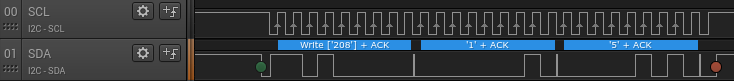
\includegraphics[scale=0.6]{coms_ds1307.png}
	\caption{}
	\label{coms_ds1307}
\end{figure}
\subsubsection{25LC640}
\begin{figure}[h!]
	\centering
	\begin{minipage}[b]{\textwidth}
		\centering
		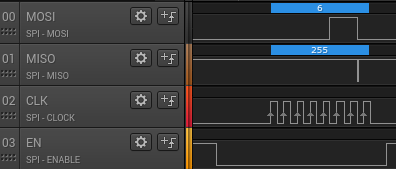
\includegraphics[scale=0.6]{coms_25lc640_start.png}
		\subcaption[first caption.]{}
		\label{fig:coms_25lc640_start}
	\end{minipage}
	\begin{minipage}[b]{\textwidth}
		\centering
		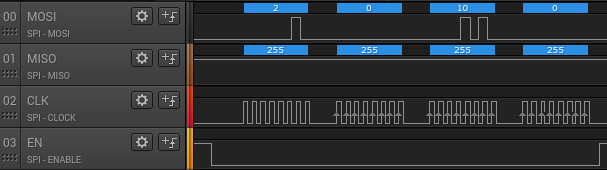
\includegraphics[scale=0.6]{coms_25lc640_data.png}
		\subcaption[second caption.]{}
		\label{fig:coms_25lc640_data}
	\end{minipage}	
	\caption{}
	\label{25lc640}
\end{figure}
\subsubsection{HC-06}
\begin{figure}[h!]
	\centering
	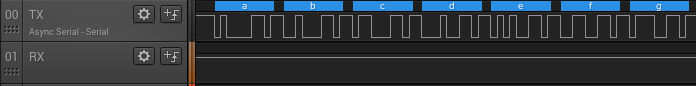
\includegraphics[scale=0.6]{coms_hc-06.png}
	\caption{}
	\label{coms_hc-06}
\end{figure}
\subsubsection{NX4024T032\_001}
\begin{figure}[h!]
	\centering
	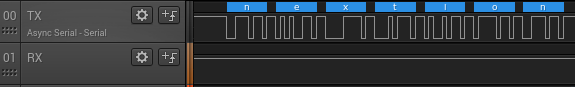
\includegraphics[scale=0.6]{coms_nextion.png}
	\caption{}
	\label{coms_nextion}
\end{figure}
\subsubsection{WS2812}
\begin{figure}[h!]
	\centering
	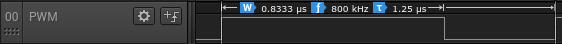
\includegraphics[scale=0.8]{coms_ws2812_frequency.png}
	\caption{}
	\label{coms_ws2812_frequency}
\end{figure}
\begin{figure}[h!]
	\centering
	\begin{minipage}[b]{\textwidth}
		\centering
		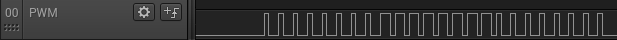
\includegraphics[scale=0.8]{coms_ws2812_red.png}
		\subcaption[first caption.]{}
		\label{fig:coms_ws2812_red}
	\end{minipage}
	\begin{minipage}[b]{\textwidth}
		\centering
		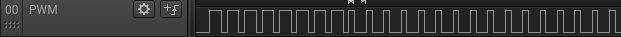
\includegraphics[scale=0.8]{coms_ws2812_green.png}
		\subcaption[second caption.]{}
		\label{fig:coms_ws2812_green}
	\end{minipage}
	\begin{minipage}[b]{\textwidth}
		\centering
		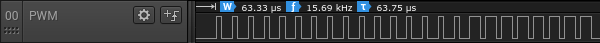
\includegraphics[scale=0.8]{coms_ws2812_blue.png}
		\subcaption[second caption.]{}
		\label{fig:coms_ws2812_blue}
	\end{minipage}	
	\caption{}
	\label{ws2812}
\end{figure}
\subsection{Discussions}


%%%%%%%%%%%%%%%%%%%%%%%%%%%%%%%%%%%%%%%%%%%%%%%%%%%%%%%%%%%%%%%%%%%%%%%%%%%%%%%%%%%%
% SECTION: Software tests
%%%%%%%%%%%%%%%%%%%%%%%%%%%%%%%%%%%%%%%%%%%%%%%%%%%%%%%%%%%%%%%%%%%%%%%%%%%%%%%%%%%%
\section{Software Tests}
\subsection{Unit Tests outcome}
\begin{table}[h!]
	\centering
	\caption{Unit and Integration test outcome.}
	\label{table:software_unit_test}
	\begin{tabular}{cccc}
		\hline
		\hline
		\toprule
		\textbf{Hardware} & \textbf{Unit test} & \textbf{Outcome} & \textbf{Coverage estimation}\\
		\bottomrule
		\toprule
		\multirow{3}{*}{internal RTC} & test\_clock\_date & Pass & \multirow{3}{*}{33.33\%}\\
		& test\_clock\_time & Pass &\\
		& test\_clock\_alarm & Pass &\\
		\midrule
		external RTC & test\_rtc\_clock & Pass & 47.1\%\\
		\midrule
		\multirow{3}{*}{queue} & test\_queue\_create & Pass & \multirow{3}{*}{44.44\%}\\
		& test\_queue\_enqueue & Pass &\\
		& test\_queue\_dequeue & Pass &\\
		\midrule
		\multirow{3}{*}{eeprom} & test\_eeprom\_write\_read & Pass & \multirow{3}{*}{66.67\%}\\
		& test\_eeprom\_write4B\_read4B & Pass &\\
		& test\_eeprom\_writeNB\_readNB & Pass &\\
		\midrule
		\multirow{2}{*}{alarm} & test\_alarm\_address & Pass & \multirow{2}{*}{66.67\%}\\
		& test\_alarm\_save\_load & Pass &\\ 
		\bottomrule
		\hline
		\hline
	\end{tabular}
\end{table}

\subsection{Insight on the software tests}

%%%%%%%%%%%%%%%%%%%%%%%%%%%%%%%%%%%%%%%%%%%%%%%%%%%%%%%%%%%%%%%%%%%%%%%%%%%%%%%%%%%%
% SECTION: Ring 
%%%%%%%%%%%%%%%%%%%%%%%%%%%%%%%%%%%%%%%%%%%%%%%%%%%%%%%%%%%%%%%%%%%%%%%%%%%%%%%%%%%%
\section{Ring experiments}

\subsection{Current drawn by the Ring}
\subsubsection{Experimental results}

\begin{table}[h!]
	\centering
	\caption{Current drawn by a one neopixel per colour at different brightness levels. The white colour is obtain by turning the red, green and blue LEDs on at the same brightness.}
	\label{table:current_one_pixel}
	\begin{tabular}{ccccc}
		\hline
		\hline
		\toprule
		\multirow{2}{*}{\textbf{Brightness (\%)}} & \multicolumn{4}{c}{\textbf{Current (mA)}}\\
		& \textbf{Red} & \textbf{Green} & \textbf{Blue} & \textbf{White} \\
		\bottomrule
		\toprule
		0	&	3	&	3	&	3	&	3	\\
		10	&	4	&	4	&	4	&	5	\\
		20	&	5	&	5	&	5	&	9	\\
		30	&	7	&	7	&	6	&	13	\\
		40	&	8	&	8	&	8	&	17	\\
		50	&	10	&	10	&	9	&	22	\\
		60	&	11	&	11	&	11	&	26	\\
		70	&	13	&	12	&	12	&	30	\\
		80	&	14	&	14	&	13	&	34	\\
		90	&	15	&	15	&	15	&	38	\\
		100	&	17	&	17	&	16	&	42	\\
		\bottomrule
		\hline
		\hline
	\end{tabular}
\end{table}

\begin{table}[h!]
	\centering
	\caption{Current drawn by the neopixels in idle mode. The idle mode is defined as the state of the of the neopixel when no light is emitted.}
	\label{table:current_idle}
	\begin{tabular}{cc}
		\hline
		\hline
		\toprule
		\textbf{Number of neopixels} & \textbf{Current (mA)}\\
		\bottomrule
		\toprule
		0	&	89	\\
		10	&	89	\\
		25	&	90	\\
		50	&	92	\\
		90	&	95	\\
		120	&	97	\\
		150	&	99	\\
		180	&	101	\\
		\bottomrule
		\hline
		\hline
	\end{tabular}
\end{table}


\begin{table}[h!]
	\centering
	\caption{Current drawn by all 180 neopixels on the Ring at different brightness levels.}
	\label{table:current_180_neopixels}
	\begin{tabular}{ccccc}
		\hline
		\hline
		\toprule
		\multirow{2}{*}{\textbf{Brightness (\%)}} & \multicolumn{4}{c}{\textbf{Current (A)}}\\
		& \multicolumn{3}{c}{\textbf{Readings}} & \textbf{Average} \\
		\bottomrule
		\toprule
		0	&	0.120	&	0.120	&	0.120	&	0.120	\\
		10	&	0.510	&	0.510	&	0.500	&	0.507	\\
		20	&	1.250	&	1.230	&	1.220	&	1.233	\\
		30	&	2.000	&	1.980	&	1.970	&	1.983	\\
		40	&	2.730	&	2.690	&	2.680	&	2.700	\\
		50	&	3.480	&	3.430	&	3.410	&	3.440	\\
		60	&	4.890	&	4.120	&	4.110	&	4.373	\\
		70	&	4.910	&	4.840	&	4.830	&	4.860	\\
		80	&	5.600	&	5.530	&	5.510	&	5.547	\\
		90	&	6.320	&	6.240	&	6.220	&	6.260	\\
		100	&	7.020	&	6.910	&	6.890	&	6.940	\\
		\bottomrule
		\hline
		\hline
	\end{tabular}
\end{table}

\begin{figure}[ht]
	\centering
	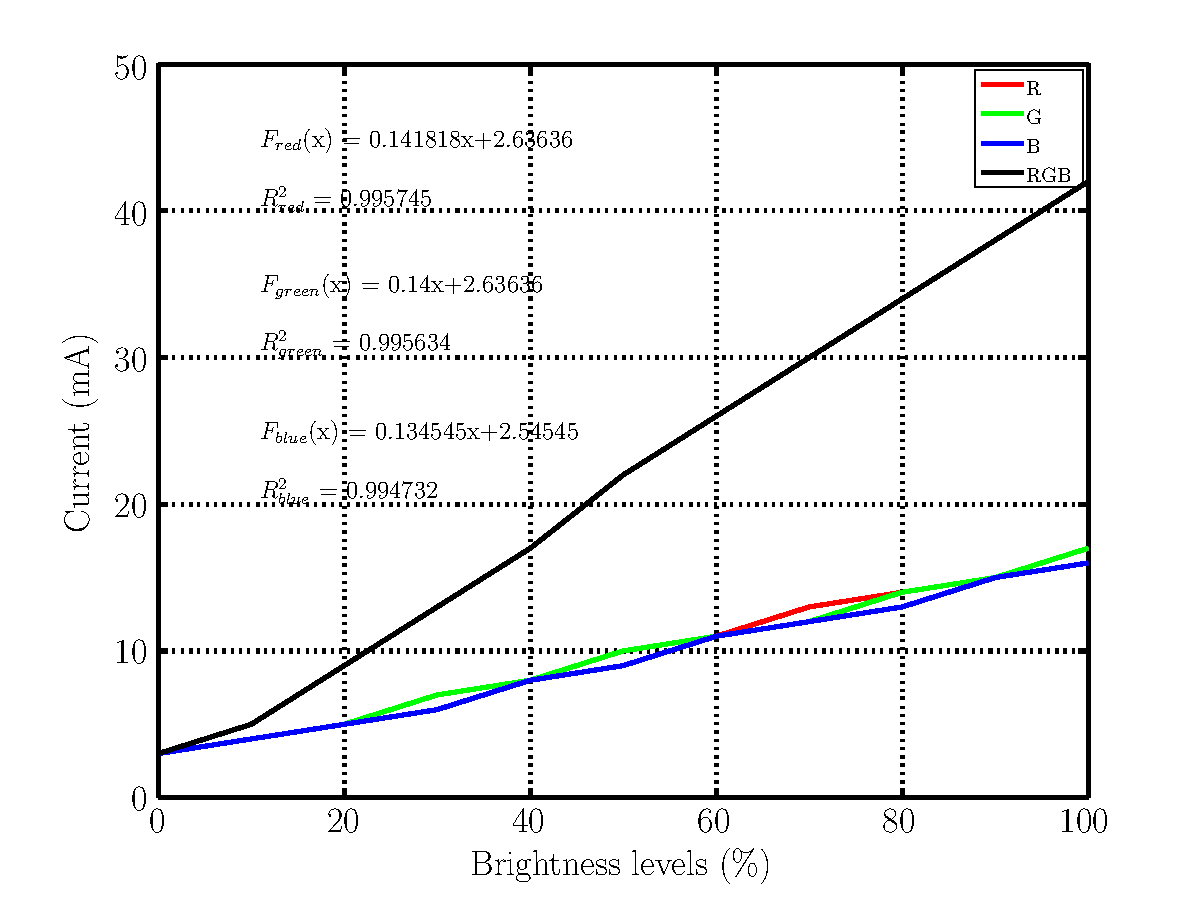
\includegraphics[scale=0.6]{current_one_pixel.pdf}
	\caption{}
	\label{fig:current_one_pixel}
\end{figure}
\begin{figure}[ht]
	\centering
	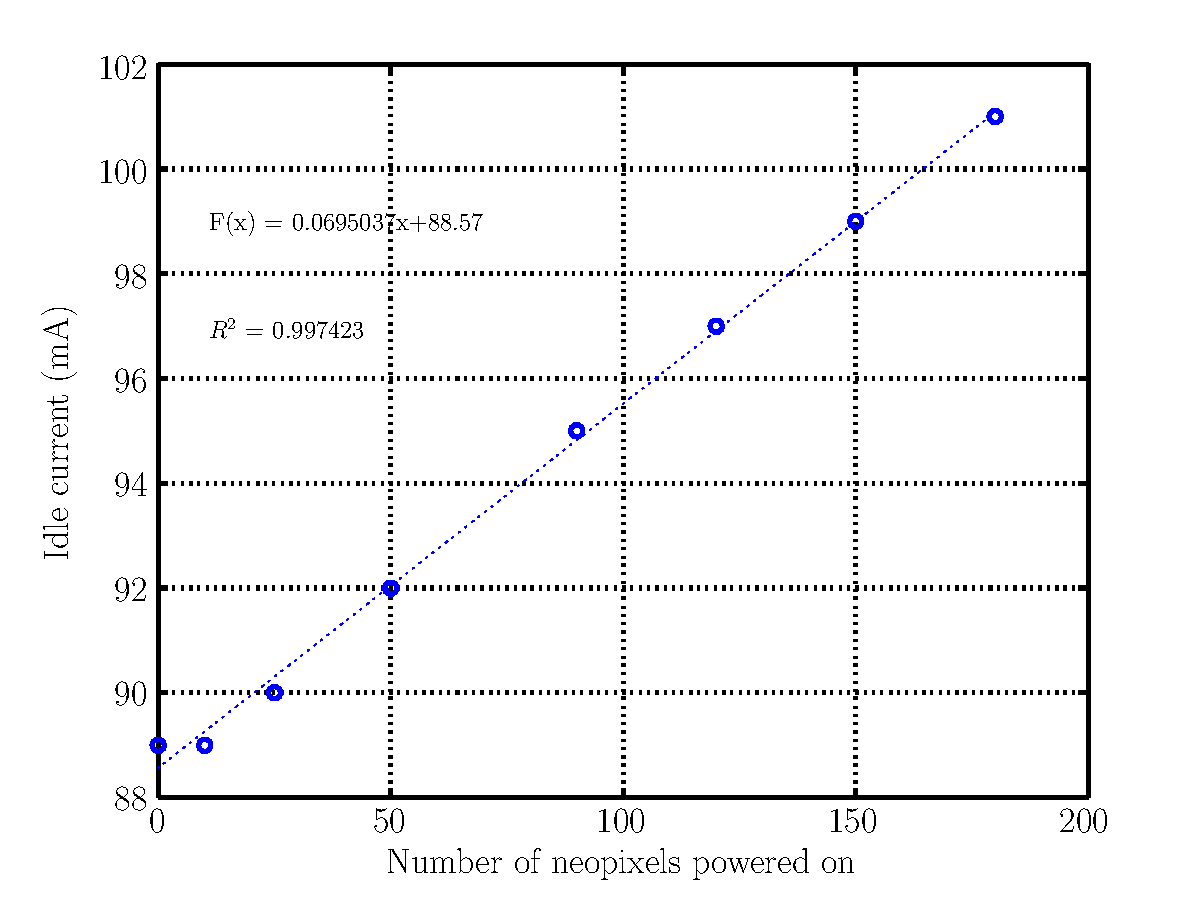
\includegraphics[scale=0.6]{current_idle.pdf}
	\caption{}
	\label{fig:current_idle}
\end{figure}
\begin{figure}[ht]
	\centering
	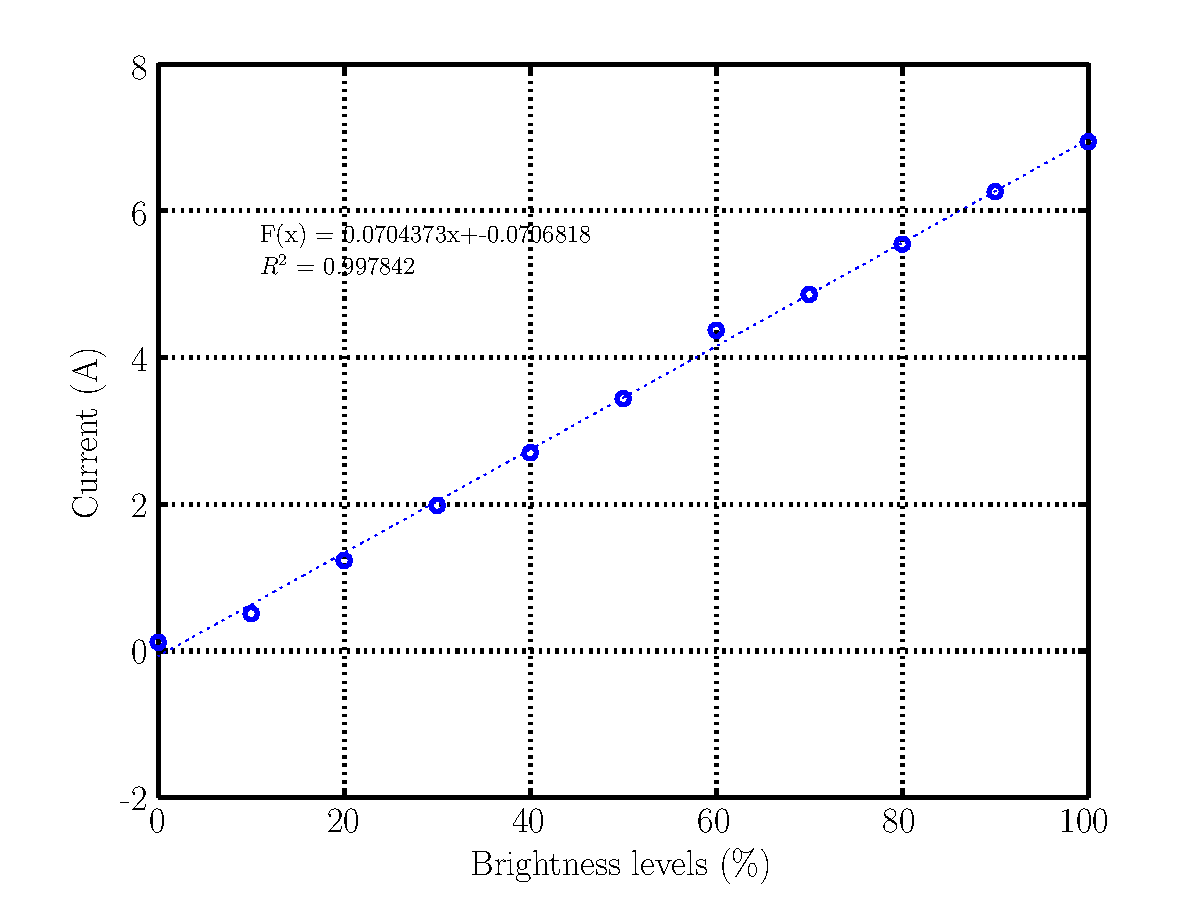
\includegraphics[scale=0.6]{current_180_neopixels.pdf}
	\caption{}
	\label{fig:current_180_neopixels}
\end{figure}

\subsubsection{Discussion}

\subsection{Ring temperature by the Ring}
\subsubsection{Experimental results}

\begin{table}[h!]
	\centering
	\caption{Current drawn by the neopixels in idle mode. The idle mode is defined as the state of the of the neopixel when no light is emitted.}
	\label{table:temperature_ring}
	\begin{tabular}{cc}
		\hline
		\hline
		\toprule
		\textbf{Current (A)} & \textbf{Temperature ($^oC$)}\\
		\bottomrule
		\toprule
		0.09	&	2.176	\\
		0.49	&	6.417	\\
		1.24	&	11.750	\\
		1.95	&	17.667	\\
		3.38	&	28.083	\\
		4.1		&	29.667	\\
		5.35	&	39.000	\\
		6		&	43.091	\\
		6.55	&	44.750	\\
		\bottomrule
		\hline
		\hline
	\end{tabular}
\end{table}
\begin{figure}[ht]
	\centering
	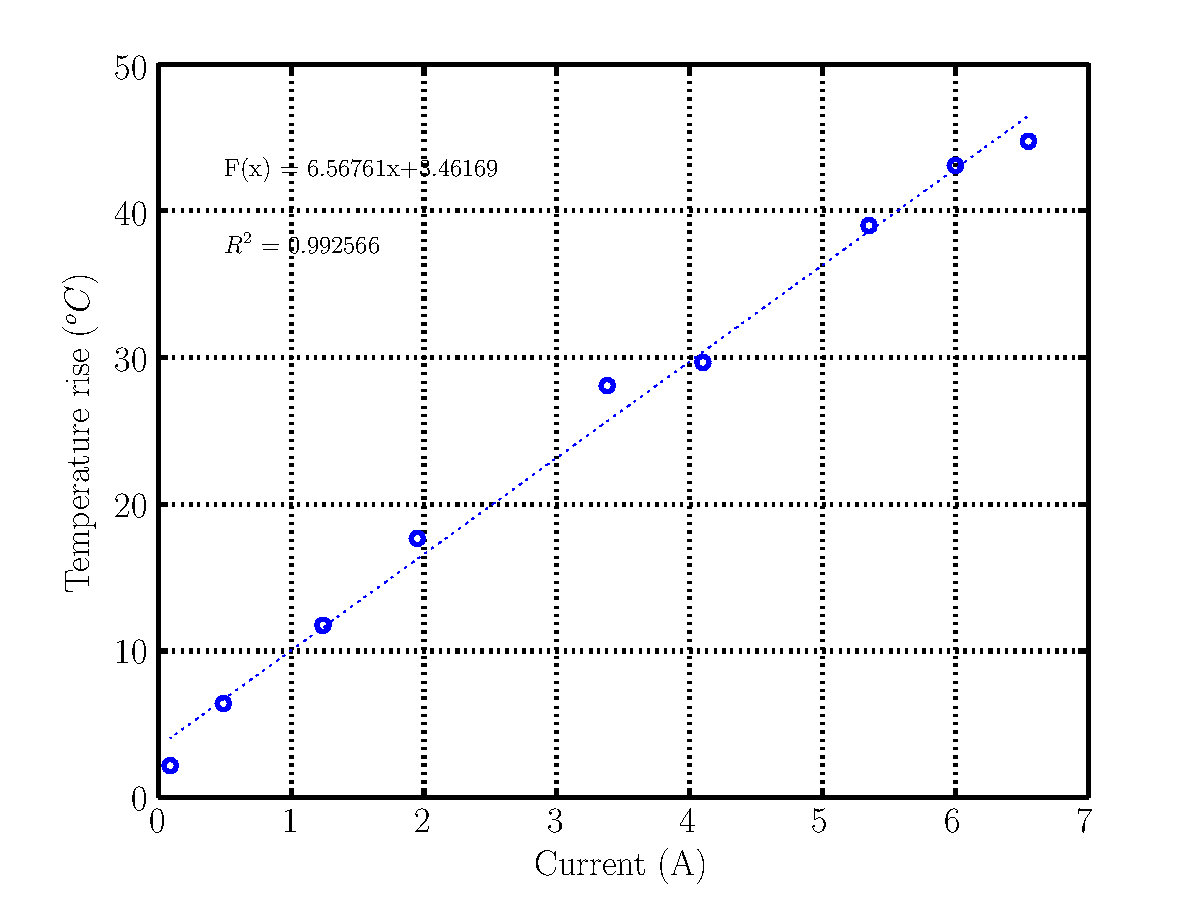
\includegraphics[scale=0.6]{temperature_ring.pdf}
	\caption{}
	\label{fig:temperature_ring}
\end{figure}

\subsubsection{Discussion}

\subsection{Illuminance produced by the Ring}
\subsubsection{Experimental results}

\begin{table}[h!]
	\centering
	\caption{Ring's blue LED illuminance at full brightness per distance and angular section to the Ring.}
	\label{table:illuminance_blue}
	\begin{tabular}{ccccc}
		\hline
		\hline
		\toprule
		\multirow{2}{*}{\textbf{Distance (cm)}} & \multicolumn{4}{c}{\textbf{Angle (deg)}}\\
		& 0 & 30 & 60 & 90 \\
		\bottomrule
		\toprule
		20	&	6420	&	5950	&	5310	&	1998	\\
		30	&	4910	&	3770	&	3302	&	547		\\
		40	&	2507	&	2354	&	1657	&	149		\\
		50	&	1820	&	1620	&	1219	&	110		\\
		60	&	1375	&	1227	&	892		&	60		\\
		70	&	1012	&	943		&	691		&	55		\\
		80	&	810		&	785		&	547		&	43		\\
		90	&	667		&	607		&	420		&	35		\\
		100	&	557		&	500		&	353		&	30		\\
		\bottomrule
		\hline
		\hline
	\end{tabular}
\end{table}
\begin{figure}[ht]
	\centering
	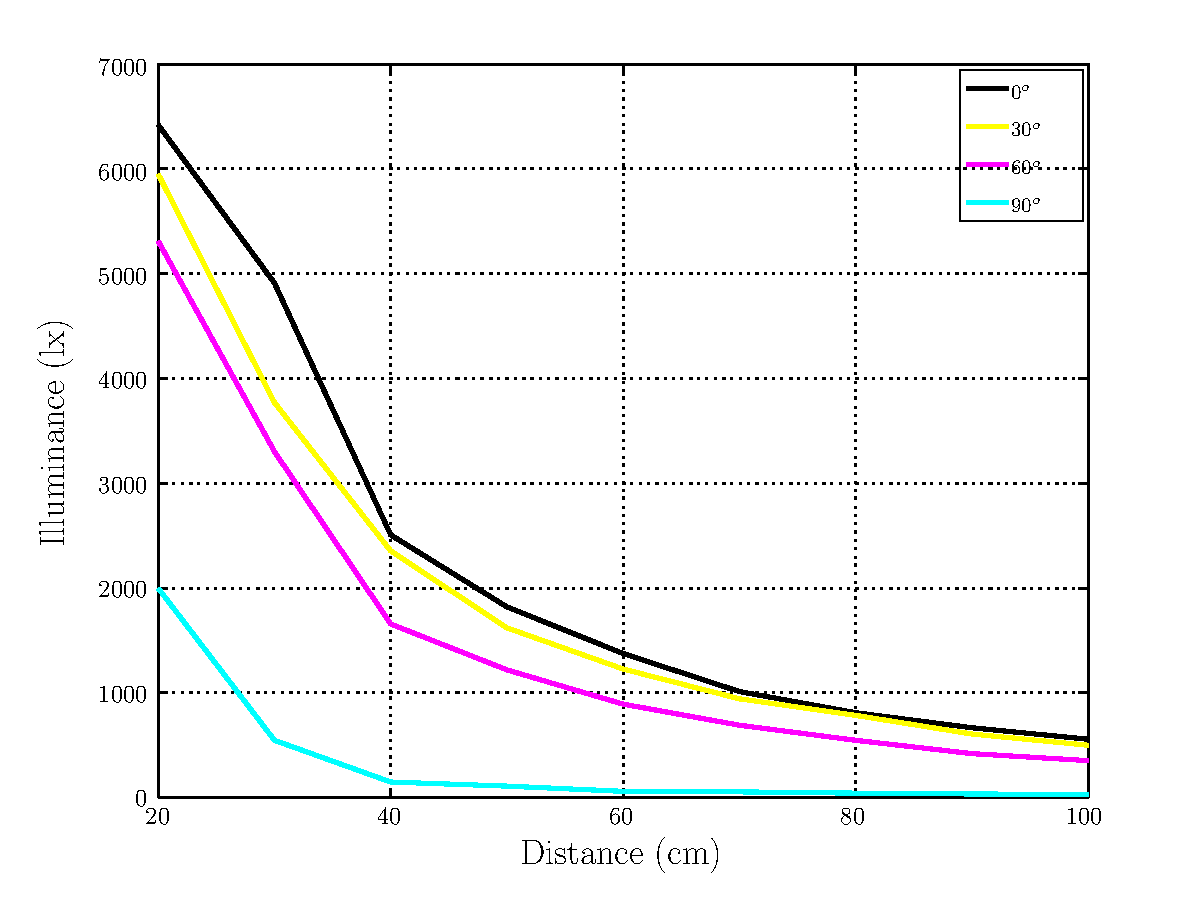
\includegraphics[scale=0.6]{illuminance_blue.pdf}
	\caption{}
	\label{fig:illuminance_blue}
\end{figure}

\begin{table}[h!]
	\centering
	\caption{Relationship between the coefficient of decadence of the Ring illuminance and the distance to the Ring.}
	\label{table:illuminance_distance}
	\begin{tabular}{cccccccc}
		\hline
		\hline
		\toprule
		\multirow{2}{*}{\textbf{Distance (cm)}} & \multicolumn{5}{c}{\textbf{Brightness (\%)}} & \multirow{2}{*}{\textbf{Average}} & \multirow{2}{*}{\textbf{Std dev}}\\
		& 10 & 30 & 50 & 80 & 90 &&\\
		\bottomrule
		\toprule
		20	&	1.00	&	1.00	&	1.00	&	1.00	&	1.00	&	1.00	&	0.00	\\
		30	&	0.68	&	0.63	&	0.65	&	0.65	&	0.59	&	0.64	&	0.03	\\
		40	&	0.44	&	0.40	&	0.44	&	0.41	&	0.36	&	0.41	&	0.03	\\
		50	&	0.31	&	0.29	&	0.31	&	0.28	&	0.27	&	0.29	&	0.02	\\
		60	&	0.23	&	0.20	&	0.23	&	0.22	&	0.20	&	0.22	&	0.01	\\
		70	&	0.18	&	0.15	&	0.18	&	0.17	&	0.15	&	0.17	&	0.01	\\
		80	&	0.14	&	0.13	&	0.14	&	0.13	&	0.12	&	0.13	&	0.01	\\
		90	&	0.12	&	0.10	&	0.11	&	0.13	&	0.10	&	0.11	&	0.01	\\
		100	&	0.10	&	0.08	&	0.09	&	0.09	&	0.08	&	0.09	&	0.01	\\
		\bottomrule
		\hline
		\hline
	\end{tabular}
\end{table}
\begin{figure}[ht]
	\centering
	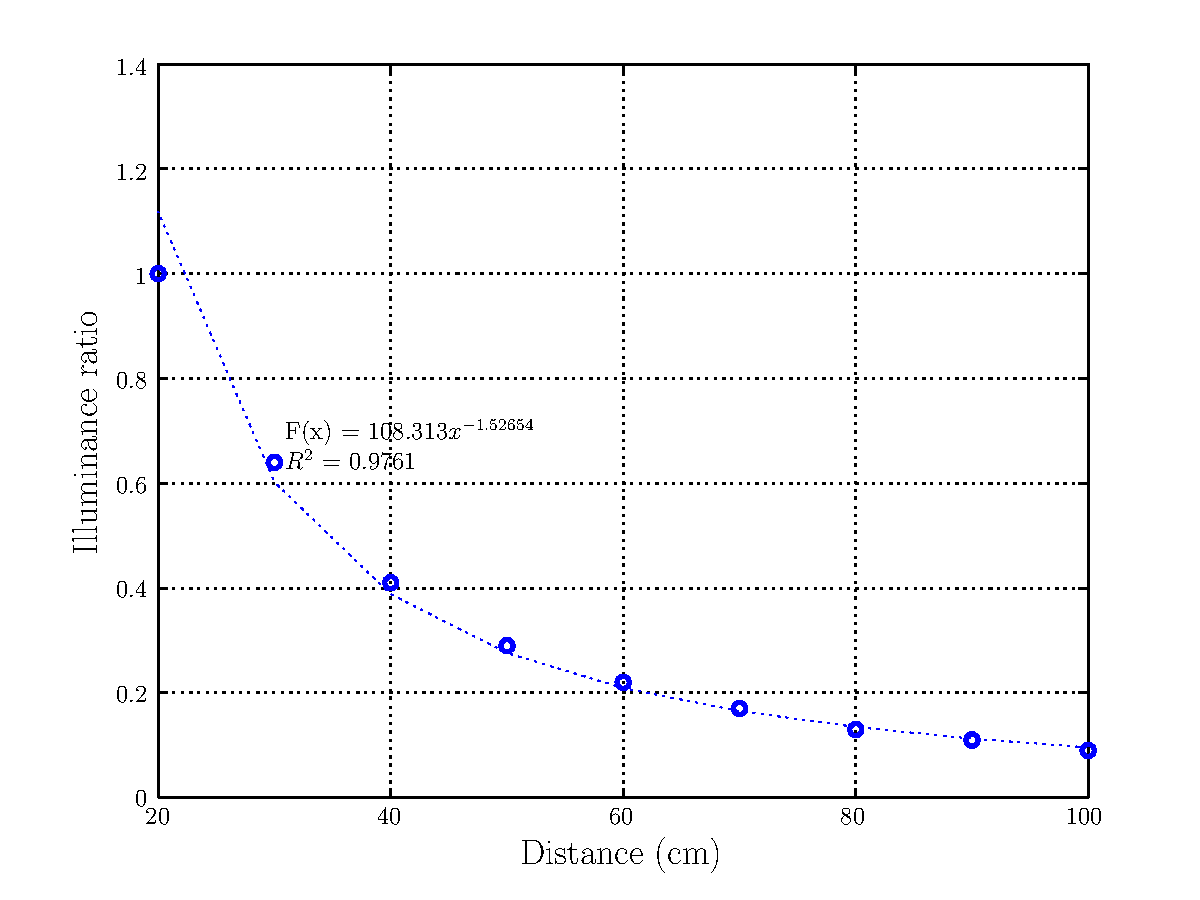
\includegraphics[scale=0.6]{illuminance_distance.pdf}
	\caption{}
	\label{fig:illuminance_distance}
\end{figure}

\begin{table}[h!]
	\centering
	\caption{Relationship between the Ring illuminance and the angle to the normal of the Ring surface.}
	\label{table:illuminance_angle}
	\begin{tabular}{cccccccc}
		\hline
		\hline
		\toprule
		\multirow{2}{*}{\textbf{Angle (cm)}} & \multicolumn{5}{c}{\textbf{Distance (cm)}} & \multirow{2}{*}{\textbf{Average}} & \multirow{2}{*}{\textbf{Std dev}}\\
		& 20 & 30 & 50 & 80 & 100 &&\\
		\bottomrule
		\toprule
		0	&	1.00	&	1.00	&	1.00	&	1.00	&	1.00	&	1.00	&	0.00	\\
		30	&	0.88	&	0.89	&	0.53	&	0.94	&	0.90	&	0.83	&	0.16	\\
		60	&	0.75	&	0.70	&	0.65	&	0.64	&	0.64	&	0.68	&	0.05	\\
		90	&	0.20	&	0.16	&	0.09	&	0.06	&	0.05	&	0.11	&	0.07	\\
		\bottomrule
		\hline
		\hline
	\end{tabular}
\end{table}
\begin{figure}[ht]
	\centering
	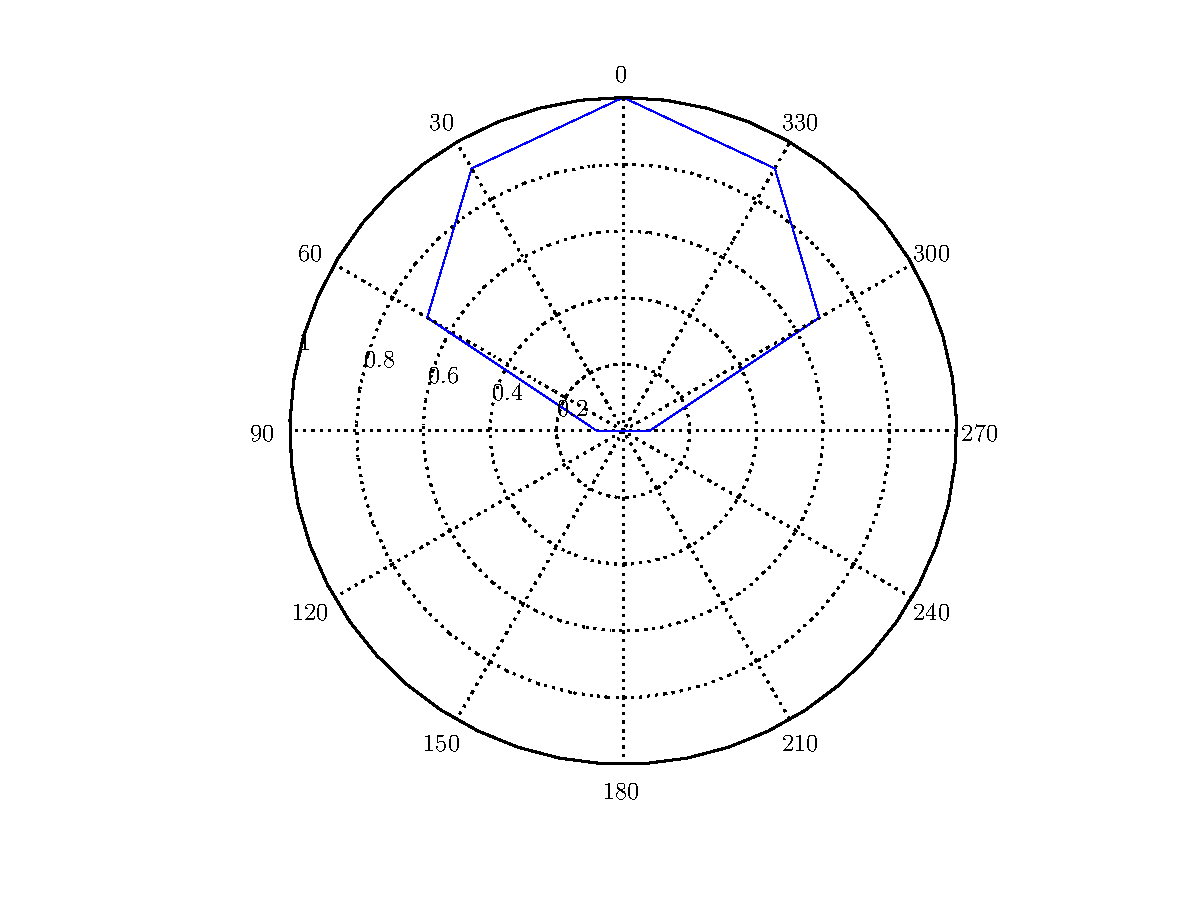
\includegraphics[scale=0.6]{illuminance_angle.pdf}
	\caption{}
	\label{fig:illuminance_angle}
\end{figure}


\subsubsection{Discussion}
\chapter{Discussion}

Here is what the results mean and how they tie to existing literature...

Discuss the relevance of your results and how they fit into the theoretical work you described in your
literature review.

\chapter{Conclusions and Recommendations}

\section{Review of objectives}
The sub-requirements set in \ref{sub_requirements} and their satisfaction level are shown in \cref{table:conclusion_subrequirements}. The table provides reasons on the satisfaction level given for each requirement.
\begin{table}[h!]
	\centering
	\caption{Sub-requirements implementation satisfaction.}
	\label{table:conclusion_subrequirements}
	\begin{tabular}{p{10em}cp{15em}}
		\hline
		\hline
		\toprule
		\textbf{Sub-requirements} & \textbf{Level of satisfaction} & \textbf{Coments}\\
		\bottomrule
		\toprule
		Onboard touchscreen & High & Good framework design for communication between screen and STM\\
		\midrule
		Smartphone App & Low & Framework is developed but actual application can only connect to bluetooth\\
		\midrule
		User preference & Medium & Framework for storing and loading any parameters have been implemented\\
		\midrule
		Set/edit alarm & High& Good framework allowing alarm configuration\\
		Set/get time and date & High & Good framework allowing time and date parameters to be stored and loaded\\
		\midrule
		Light parameters & Good & Framework allows configuration of the neopixels colour and brightness.\\
		\midrule
		Light pattern & Low & Data sent to neopixels is corrupted by the interrupt generated by other module\\
		\bottomrule
		\hline
		\hline
	\end{tabular}
\end{table}
Each of these sub-requirements is related to the system requirement. \Cref{table:conclusion_requirements} provides the satisfaction lvel of the system requirements. 
\begin{table}[h!]
	\centering
	\caption{Requirements implementation satisfaction.}
	\label{table:conclusion_requirements}
	\begin{tabular}{cc}
		\hline
		\hline
		\toprule
		\textbf{Requirements} & \textbf{Level of satisfaction}\\
		\bottomrule
		\toprule
		Visual & Low \\
		\midrule
		Instruction & High \\
		\midrule
		Alarm & High \\
		\bottomrule
		\hline
		\hline
	\end{tabular}
\end{table}
\subsection{Instruction and user inputs}
The instruction application provided a solid foundation for the implementation of the applications running on each input device. The Nextion touchscreen application provides a nice and easy user interaction with the NPSC. The smartphone application is not fully implemented, the basic interaction provided by this application was connecting the smartphone to the NPSC system. 
\subsection{Alarm}
The alarm application successfully managed the time, date and alarm information of the system. The user has full control of the time, date and the alarm to be set.  
\subsection{Visual}
The visual module was able to control the neopixel at a module level. However, it failed once it was integrated with other modules as they interupted the stream of data sent to the neopixel. For this reason the visual application could not be fully implemented.

\paragraph{Objectives}
\textit{The purpose of this study is to create a device that can be used to regulate the human sleep-wake cycle while being user-friendly and a personalisable digital alarm clock.} \\
The objectives are reviewed in \Cref{table:conclusion_objectives}.
\begin{table}[h!]
	\centering
	\caption{Review of objectives.}
	\label{table:conclusion_objectives}
	\begin{tabular}{p{20em}c}
		\hline
		\hline
		\toprule
		\textbf{Objectives} & \textbf{Comment}\\
		\bottomrule
		\toprule
		The device is capable of producing light of $460\pm10nm$ wavelength at an illuminance of $30lx$ & \checkmark \\
		\midrule
		The device is an alarm clock & \checkmark \\
		\midrule
		The device is user-friendly & \checkmark \\
		\midrule
		The device has more features than its competitors & X \\
		\bottomrule
		\hline
		\hline
	\end{tabular}
\end{table}  

\section{Reflections on the design}
The prototype of the NPSC is proof that the neopixels can be used to create a device capable of affecting the human sleep-wake cycle. However, using a large number of neopixels in an embedded system requires careful use of the microcontroller resources. In this project, the DMA was not used to control the neopixel resulting in the CPU doing all the work from the communication between all modules to the transmission of the neopixels' data. \\
The prototype is subjective to many design changes, therefore, a cost analysis could not be performed. Considering all the module designed for the neopixel, a significant amount of work has been done. All modules have been tested and proven to work creating a solid foundation for future improvements. 

\section{Recommendation for future work}
The following recommendations are firstly made so that all requirements established in the introduction are met, secondly do that the NPSC's design and performance increases over time.\\
The recommendations are the following:
\begin{itemize}
	\item The NPSC's visual module should be dedicated to another microcontroller, preferably an STM32F0 so that the libraries made can be reused. The role of the STM32F0 would solely be to read instruction from the STM32F4 and update the visual output accordingly. This would reduce the workload of the STM32F4 and physically separate the visual module from the other module. 
	\item The neopixel library should make use of the Direct Memory Access (DMA) to reduce the CPU workload.
	\item The experiment performed on the Ring should be done in a completely dark room where the reflection would be minimum to increase the reading accuracy
\end{itemize}
\chapter{Recommendations}

Make sensible recommendations for further work.

Use the IEEE numbered reference style for referencing your work as shown in your thesis guidelines.
Please remember that the majority of your referenced work should be from journal articles, technical
reports and books not online sources such as Wikipedia.

\begin{thebibliography}{5}
\bibitem{smt2011} M. S. Tsoeu and M. Braae, ``Control Systems,'' \emph{IEEE}, {\bf vol. 34(3)}, pp. 123-129, 2011.
\bibitem{jct2010} J. C. Tapson, \emph{Instrumentation}, UCT Press, Cape Town, 2010.
\end{thebibliography}

\appendix
\chapter{Additional Files and Schematics}

Add any information here that you would like to have in your project but is not necessary in the main
text. Remember to refer to it in the main text. Separate your appendices based on what they are for
example. Equation derivations in Appendix A and code in Appendix B etc.

\chapter{Addenda}

\section{Ethics Forms}

}
\end{document}
